%\documentclass[a4paper,12pt,fleqn,twoside]{scrbook}
\documentclass[a4paper,11pt, twoside, openright]{scrbook}

\usepackage[T1]{fontenc}
\usepackage{ucs}
\usepackage[utf8x]{inputenc}
\usepackage{ngerman}
\usepackage[ngerman]{babel}
\usepackage{lastpage}
\usepackage[pdftex]{color,graphicx}
\usepackage{listings}
\usepackage{pdflscape}
\usepackage{longtable}
\usepackage[font=sf, labelfont={sf}, margin=1cm,size=small]{caption}

%\usepackage{showframe}
\usepackage[lmargin=130pt,rmargin=80pt,tmargin=117pt,bmargin=113pt]{geometry}
%\usepackage[inner=2cm,outer=2cm,top=1cm,bottom=1.5cm,includeheadfoot]{geometry}

\usepackage{fancyhdr}
\usepackage{url}

\usepackage{booktabs}
\usepackage{blindtext} 
\usepackage{lipsum}

\usepackage{framed} 
\usepackage{xcolor} 
\colorlet{shadecolor}{black} 
\usepackage{latexsym}
\usepackage{float}

\usepackage{bbm}
\usepackage{enumitem}

%\usepackage{draftwatermark}
%\SetWatermarkText{Entwurf}
%\SetWatermarkScale{4}
%\SetWatermarkLightness{0.9}
\usepackage[section]{placeins}
\usepackage{pgfgantt}
\usepackage{amsmath,amssymb,amsfonts,amstext}
\usepackage{floatflt}
\usepackage{tikz}
\usetikzlibrary[arrows,snakes,backgrounds,shapes]
\usetikzlibrary{through}
\usetikzlibrary{calc}
\usepackage{caption}
\usepackage{subcaption}
\usepackage{wrapfig}
\usepackage{makeidx}
\usepackage{transparent}
%\usepackage{nimbus}
% highlighting
\usepackage{xcolor,soul}
\usepackage{threeparttable}
%\renewcommand{\sectionmark}[1]{\markboth{#1}{#1}} 
%\renewcommand{\subsectionmark}[1]{\markboth{#1}{}} 

%---- PageLayout
\pagestyle{fancy}

%\setlength{\textheight}{225mm}
%\setlength{\headsep}{20mm}
\usepackage{eso-pic}
%\usepackage[numbers,round]{natbib}

%----------------------------------------------------------------------------
% HEADER --------------------------------------------------------------------
%----------------------------------------------------------------------------
%\fancyhead[R]{
%  
\includegraphics[width=100pt,keepaspectratio]{img/amedo2012.png}
%}

%\fancyhead[C]{ }

\fancyhead[RO]{
\thepage{}
}
%\fancyhead[RE]{}
%\fancyhead[LO]{}
\fancyhead[LE]{
\thepage{}
%  \begin{tabular}[b]{l}
%  Christoph Gnip\\
%  Projekt: PRPS-Evolution
%  \end{tabular}
}

%Linie oben
\renewcommand{\headrulewidth}{0.5pt}
%----------------------------------------------------------------------------

%----------------------------------------------------------------------------
%----------------------------------------------------------------------------
%----------------------------------------------------------------------------
%\fancyfoot[L]{Stand: \today}
\fancyfoot[C]{ Entwurf }
\fancyfoot[R]{\thepage{} von \pageref{LastPage}}

% Linie unten
\renewcommand{\footrulewidth}{0.5pt}
%----------------------------------------------------------------------------

% Import Macros  ------------------------------------------------------------
\newcommand\nn{\newline\newline}

%----------------------------------------------------------------------------
% Start the Document --------------------------------------------------------
%----------------------------------------------------------------------------
\begin{document}
\frontmatter 

%\setlength{\headheight}{36pt}

%----------------------------------------------------------------------------
% Titlepage -----------------------------------------------------------------
%----------------------------------------------------------------------------

%- the Title page --------------------------------------------------------
\begin{titlepage}
       \begin{center}
           %\vspace*{2.5cm}
			{
			\Huge 
			\textbf{
			  Entwicklung eines Systems zur
			  Entfernungsabschätzung für Phasen basiertes UHF RFID Tracking durch Verwendung
			  evolutionärer Berechnungsverfahren
			}\par
			}
			\vspace{3cm}
			{
			\Large Masterthesis eingereicht zur Erfüllung\\
			der Anforderungen zum Erwerb des akademischen Grades\\
			Master of Science der Medizintechnik\\
			}
\vspace{2cm}

\large{Erstellt von}\\

\Large{\textbf{Christoph Gnip}}


%\vspace{4cm}
\vfill

{\normalsize Department Electrical Engineering and Applied Sciences
           \\Wesphalian University of Applied Sciences\\[2ex]February 2013}


       \end{center}
   \end{titlepage}

\newpage
\pagenumbering{roman}
\thispagestyle{empty}
\hspace{1cm}

\newpage
%\vspace{1cm}
\normalsize


\begin{longtable}{p{4cm}p{95mm}}
{} & {}\\
\Large{Master's Thesis} & {}\\
{} & {}\\
{} & {}\\
Titel: & Entwicklung eines Systems zur
Entfernungsabschätzung für Phasen basiertes UHF RFID Tracking durch Verwendung
evolutionärer Berechnungsverfahren\\
Title: & Development of a Distance Estimation System for
Phase-Based UHF RFID Tracking by Utilizing Methodes of Evolutionary Computation\\
{} & {}\\
{} & {}\\
University:                 & Westphalian University of Applied Sciences \\
{} & Department Electrical Engineering and Applied Sciences \\
{}                          & Neidenburger Str. 43 \\
{}                          & 45897 Gelsenkirchen \\
{}                          & Germany \\
{}                          & {}\\
{}                          & {}\\
In Cooperation with:        & Amedo Smart Tracking Solutions GmbH\\
{}                          & Universitätstraße 142 \\
{}                          & Bochum \\
{}                          & {}\\
Author:                     & Christoph Gnip \\
{}                          & Luggendelle 28 \\
{}                          & 48954 Gelsenkirchen \\
{}                          & Germany \\
{}                          & {}\\
Matrikelnumber:			& 200720362 \\
{}                          & {}\\
Supervisor:                 & Prof. Dr. Frank Bärmann \\
Co-supervisor:              & Dipl.-Ing. Volker Trösken\\
\end{longtable}

\newpage


\Large{\textbf{Erklärung}}\\
%
%
\\
\\
\normalsize
Hiermit erkläre ich, dass ich die Vorliegende Arbeit selbständig und lediglich mit den angegebenen Hilfsmittel verfasst habe...
%
\newpage

%
\Large{\textbf{Dank und Anerkennung}}\\
\\
\\
\normalsize
Danke...
%
\newpage
\newpage

\pagenumbering{roman} 

%----------------------------------------------------------------------------
% Tables --------------------------------------------------------------------
%----------------------------------------------------------------------------
\tableofcontents 
%
\listoffigures
%
\listoftables
%
\lstlistoflistings
%
\newpage
%
\subsection*{Verwendete Abkürzungen}
%
\begin{table} [H]
	\begin{center}
		\begin{tabular}{p{25mm}p{95mm}}
		      	\textbf{ES} & Evolutionäre Strategie (\textit{Evolutionary Strategy})\\
		      	\textbf{CMA-ES}  & Covariance Matrix Adaption - Evolutionary Strategy\\
		      	\textbf{\cpp11} & Programmiersprache C++ in der Version 11\\
		      	\textbf{MRT}	& Magnetresonanztomografie\\
		      	\textbf{RFID} & Radio-Frequency Identification\\
		      	\textbf{LOS} & Line of Sight\\
		      	\textbf{CSV} & Comma seperated Values\\
		      	\textbf{Rö} & Röntgen\\
		      	\textbf{CT} & Computertomografie\\
		      	\textbf{EM} & Elektromagnetismus\\
		      	\textbf{TAG} & Transponder/ Receiver für Funk Kommunikation\\
		      	\textbf{Tracking} & Positionsbestimmung\\
		      	\textbf{PRPS} & Passiv RFID Positioning System - Produkt der \amedogmbh \\
		      	\textbf{TOF} & Time Of Flight\\
		      	\textbf{PD} & Phasendifferenz\\
		      	\textbf{RSSI} & Indikator für die empfangene Signalstärke (Received Signal Strength Indication)\\
		      	\textbf{CMake} & Cross-Platform make; Werkzeug für Erstellung von Software\\
		      	\textbf{ETSI} & European Telecommunications Standards Institute
%		      	
		\end{tabular}
	\end{center}
\end{table}


%
\newpage
\subsection*{Verwendete Symbole}
Folgende Nomenklatur und Symbole werden in dieser Arbeit verwendet
\begin{itemize}
	\item	$k$ ist der Index der Antennen im Aufbau verwendeten Antennen
	\item	Matrizen werden mit fetten Großbuchstaben notiert (bspw. $\mathbf{A}$)
	\item	Vektoren werden mit fetten Kleinbuchstaben notiert (bspw. $\mathbf{b}$)
	\item	$r_{k}$ := Abstand vom Tag zur Antenne
	\item	$d_{k0}$ := Abstand zur Landmarke
	
\end{itemize}


\mainmatter 

%\setkomafont{caption}{\footnotesize\itshape}
%\setkomafont{captionlabel}{\usekomafont{caption}}


\widowpenalty=1000
\clubpenalty=1000

%----------------------------------------------------------------------------
% Chapters ------------------------------------------------------------------
%----------------------------------------------------------------------------
% 1. ------------------------------------------------------------------------
\chapter{Einleitung}
%
%-----------------------------------------------------------------------
\section[Motivation]{Motivation}
Die Positionsbestimmung mittels RFID ist eine vielversprechende Technik. Die Bestimmung der Position (im Folgenden "Tracking" genannt) mittels RFID  bietet gegenüber vergleichbaren Methoden (z.B. Ultraschall, Optisch) verschiedene Vorteile. Das wesentlichste Unterscheidungsmerkmal ist, dass keine direkte Sichtlinie sog. LOS notwendig ist um ein Objekt zu lokalisieren. Der Grund dafür ist das zugrunde liegende Messprinzip. Es werden elektromagnetische Signale ausgewertet, die anderen Wechselwirkungen unterliegen und somit Materie durchdringen. Insbesondere im Vergleich mit optischen Verfahren ist RFID damit überlegen. Die Eigenschaft Materie zu durchdringen erlaubt es Tags im Patienten zu lokalisieren, entsprechende Untersuchungen über die Positionsgenauigkeit im Körper sind vielversprechend.[REFERENZEN]\\
Auf den Tags können zusätzliche Informationen hinterlegt werden, beispielsweise eine Identifikationsnummer oder Ähnliches. Dadurch wächst das Anwendungsspektrum weiter[REFERENZEN]. Das Auslesen von zusätzlichen Informationen ist mit keiner der anderen Technologien möglich.\\
Das von dem Messsystem der {Amedo GmbH} verwendete Verfahren basiert auf der Messung der Phasenlage der Antwort eines Tags. Die Phasenlage ist direkt proportional zu einer Entfernung, sie ist jedoch nicht Eindeutig (siehe \ref{sec:Measurement1})\\

Eine analytische Lösung des Problems ist schwierig und bisher nicht gelungen. Diese Ansätze scheiterten an der Komplexität des Problems\footnote{siehe \ref{sec:Komplexity1} und \ref{sec:Komplexity2}} oder benötigen sehr aufwändige Messreihen mit großer Anzahl an Messpunkten \cite{amedo1}. Das limitiert die Praxistauglichkeit der Verfahren.\\

In dieser Arbeit soll mittels Evolutionärer Verfahren die beschriebenen Probleme zu gelöst werden. Im Endergebnis soll dabei eine Abschätzung der Wellenzahl \ref{eq:wavenumber} möglich sein.
%
%-----------------------------------------------------------------------
\section{Voraussetzungen}
%
Dieses Kapitel stellt die Grundlagen dieser Arbeit vor. Zuerst werden mathematische und technische Grundlagen erläutert, anschließend wird das Messsystem der amedo GmbH vorgestellt.
%
%-----------------------------------------------------
\subsection[mathematisches]{Mathematische Voraussetzungen}
%
\subsection{Kondition}
%
Gegeben ist ein lineares Gleichungssystem der Form:
$$ \mathbf{A}\mathbf{x}-\mathbf{b} =\mathbf{0} $$
Eine numerische Lösung führt in der Regel zu einer von $\mathbf{0}$ verschiedenen Lösung (insbesondere bei überbestimmten Systemen), so das wir:
$$ \mathbf{A}\mathbf{\tilde{x}}-\mathbf{b} =\mathbf{r} $$
schreiben. Man nennt $\mathbf{r}$ den Residuumvektor. Es ist offensichtlich, dass ein kleines Residuum nicht hinreichend ist um von einem kleinen relativen Fehler auszugehen.\\
Weiter folgt aus $\mathbf{A}\mathbf{x}-\mathbf{b} =\mathbf{0}$ und $\mathbf{A}\mathbf{\tilde{x}}-\mathbf{b} =\mathbf{r}$,dass 
$$ \mathbf{A}\Delta\mathbf{x}=\mathbf{r}$$
und damit:
$ 
\lVert \mathbf{b} \rVert=\lVert \mathbf{Ax} \rVert \leq \lVert \mathbf{A} \rVert \lVert \mathbf{x} \rVert
$, 
$
\lVert \Delta\mathbf{x} \rVert=\lVert -\mathbf{A^{-1}r} \rVert \leq \lVert \mathbf{A^{-1}} \rVert \lVert \mathbf{r} \rVert
$
Wir können nun für den relativen Fehler schreiben:
$$
\frac{\lVert \Delta\mathbf{x} \rVert}{\lVert \mathbf{x} \rVert} \leq 
\frac{\lVert \mathbf{A^{-1}} \rVert \lVert \mathbf{r} \rVert}{\lVert \mathbf{b} \rVert / \lVert \mathbf{A} \rVert} =
\lVert \mathbf{A} \rVert \lVert \mathbf{A^{-1}} \rVert \frac{\lVert \mathbf{r} \rVert}{\lVert \mathbf{b} \rVert}
$$
Der Term $\lVert \mathbf{A} \rVert \lVert \mathbf{A^{-1}} \rVert := \text{cond}(\mathbf{A})$ heißt Konditionszahl. Auch der Begriff Konditionsmaß ist gebräuchlich und bezieht sich auf die gewählte Matrixnorm.
Es kann gezeigt werden, dass $\text{cond}(\mathbf{A}) \gg 1$  für eine schlechte Konditionierung der Matrix steht. Wird im Folgenden von einer speziellen Matrixnorm gesprochen schreiben wir $\text{cond}(\mathbf{A})$ zu 
$$ 
\text{cond}_k(\mathbf{A}) = \lVert \mathbf{A} \rVert_k \lVert \mathbf{A^{-1}} \rVert_k
$$ \\
Der Index $k$ wird entsprechend für die verwendete Norm ersetzt. Beispielsweise ergibt sich für die Konditionszahl der Spektralnorm\footnote{\url{http://de.wikipedia.org/w/index.php?title=Spektralnorm&oldid=118988565}}:
$$ 
\text{cond}_2(\mathbf{A}) = \lVert \mathbf{A} \rVert_2 \lVert \mathbf{A^{-1}} \rVert_2=
\sqrt{\frac{\mu_{max}}{\mu_{min}}}\\
$$
Die Symbole $\mu_{max}$ und $\mu_{min}$ stehen für die Eigenwerte des Systems.\\

Die Konditionszahl ermöglicht eine Analyse der Güte einer Lösung, die mittels Numerischer Verfahren ermittelt wurde. Nach \cite{hermann2006numerische} kann man folgende Aussage über die Konditionszahl treffen:
%
\begin{quote}
"Wird ein lineares Gleichungssystem $Ax=b$ mit $t$-stelliger dezimaler Gleitpunktarithmetik gelöst und beträgt die Konditionszahl $\text{cond}(A) \approx10^\alpha$, so sind auf Grund der im allgemeinen unvermeidbaren Fehler in den Eingabedaten $A$ und $b$ nur $t-\alpha-1$ Dezimalstellen der berechneten Lösung $\tilde{x}$ (bezogen auf die betragsgrößte Komponente) sicher."
\end{quote}

\subsection{SVD}
%Um die Konditionszahl zu bestimmen sind aufwändige Berechnungen\footnote{siehe Wochenbericht KW 22} der Eigenwerte der Matrix notwendig. Es wurde nach eine Möglichkeit gesucht diese effizient abzuschätzen oder zu berechnen. Vor Allem soll es auch möglich sein mit dem Verfahren eine nicht symmetrische, nicht quadratische.\\
%Eine Methode die diese Anforderungen erfüllt, ist die sog. Singulärwertzerlegung (im Folgenden SVD := engl. Singular Value Decomposition). 
Bei dem Verfahren der Singular Value Decompostion (oder auch Singulärwertzerlegung), kurz SVD, handelt es sich um eine Faktorisierung einer Matrix. Die Matrix wird dabei als Produkt von drei Matrizen dargestellt. Diese Matrizen enthalten die sog. Singulärwerte und können aus einer der Matrizen abgelesen werden. Die Eigenschaften des Systems sind, ähnlich den Eigenwerten, aus den Singulärwerten bestimmbar. Besonders an der SVD ist, die Existenz für jede Form von Matrix - einschließlich nicht quadratischer Matrizen.\\
Die SVD basiert auf folgender Theorie der linearen Algebra: Jede $M \times N$ Matrix $\mathbf{A}$ kann als Produkt einer $M \times N$ Spalten-orthogonalen Matrix $\mathbf{U}$, einer $N \times N$ Diagonalmatrix $\mathbf{\Sigma}$ mit Werten $\geq 0$ und einer dritten adjungierten $N \times N$-Matrix $\mathbf{V^*}$, so ergibt sich:
%
\begin{equation}
\mathbf{A}= \mathbf{U \Sigma V^*} = \mathbf{U \Sigma V}^T
\end{equation}
Ist $\mathbf{A}$ eine reelwertige Matrix gilt: $ \mathbf{V^*} = \mathbf{V}^T $. Die Matrix $\mathbf{ \Sigma }$ ist im Rahmen dieser Arbeit von besonderem Interesse, denn sie enthält die Singulärwerte $\sigma_r$. Ihre Gestalt ist wie folgt:
%
\begin{equation}
	\mathbf{\Sigma} = \left(\begin{array}{ccc|ccc}
	\sigma_1 &          &          &        & \vdots &        \\
	         & \ddots   &          & \cdots & 0      & \cdots \\
	         &          & \sigma_r &        & \vdots &        \\
	\hline
	         &  \vdots  &          &        & \vdots &        \\
	\cdots   &  0       & \cdots   & \cdots & 0      & \cdots \\
	         &  \vdots  &          &        & \vdots &        \\
	
	\end{array}\right)\nonumber
\end{equation}
%
\phantomeq{\mathbf{\Sigma} = }{ ,wobei~\sigma_1\geq\sigma_2\geq\cdots\geq\sigma_r> 0 \nonumber}
%
Da die $\sigma_r$ der Matrix mit den Eigenwerten in Verbindung stehen, kann aus dieser Matrix die Konditionszahl bestimmt werden. Sie ist durch folgendes Verhältnis gegeben: 
\begin{equation}
	\label{eq:cond_from_svd}
	cond(\mathbf{A})=\frac{max(\sigma_r)}{min(\sigma_r)}=\frac{max(\sigma_1)}{min(\sigma_r)}
\end{equation} 

Es gibt bereits viele Implementationen des Verfahrens, z.B. \cite{press2007numerical}. Diese Implementation wird durch den Erwerb der entsprechenden Lizenz im Rahmen dieser Arbeit verwendet. Weitere Informationen zum Verfahren sind z.B. in \cite[Kaptiel 4.6.3]{bronstejn2012taschenbuch} zu finden.
%
%-----------------------------------------------------
\subsection[technisches]{Technische Voraussetzungen}
In diesem Abschnitt werden die technischen Grundlagen für diese Arbeit vorgestellt und das Wichtigste erörtert. Es kann nicht im vollem Umfang auf die Details der Technik eingegangen werden ohne den Rahmen dieser Arbeit zu sprengen. Interessierte sei die referenzierte Literatur für eine weite Lektüre empfohlen.
%
\subsection{RFID}
\label{sec:Measurement1}
%
\begin{enumerate}
	\item Die Messung der Position erfolgt über die Auswertung der Phasenlage des empfangenen Signals in Bezug auf ein Referenzsignal. In der EU gibt es verschiedene, zulässige RFID-Frequenzen\footnote{text} (865,5?867,5 MHz) kann man die Wellenlänge mit: $ \lambda\simeq0,35 m $ angeben. Daraus folgt, dass alle 35 cm die gleiche Konfiguration der Phase vorliegt. In dieser Arbeit wird dieser Umstand Isophasen genannt. Die gewonnene Information aus der Phase ist somit redundant, d.h. es lässt sich durch die Kenntnis der Phase nicht unmittelbar auf die korrekte Postion schließen. Man kann das Problem umgehen in dem man auf die errechnete Position ein ganzzahliges Vielfaches der Wellenlänge addiert. Die sog. Wellenzahl (vgl.~\eqref{eq:Wavenumbers}).
	\item Das System der Amedo STS verwendet eine spezielle Antennenanordnung um die Position zu ermitteln. Dabei wird eine Antennenanzahl >4 eingesetzt. Für jede dieser Antennen muss eine eigene Wellenzahl bestimmt werden. Durch Auslöschung des Signals, Absorption etc. kann es dazu kommen, dass eine Antenne eine unbestimmte Zeit lang kein Signal vom Tag empfängt. Wenn die Antenne nach dieser Zeit erneut ein Signal empfängt ist die ihr zugehörige Wellenzahl unbekannt und muss neu bestimmt werden. 
	\item In realen Umgebungen treten zusätzlich noch Ruflektionen und ein sog. Multipath-Effekt auf. Dabei wird das Signal nicht auf dem Direkten Weg Antenne-Tag-Antenne empfangen sondern über einen unbekannten, längeren Weg. Dadurch kommt es zu einem Fehler in der Phase. Zusätzlich ist dieser Effekt individuell für jede Antenne.
\end{enumerate}
\lipsum[1-2]

%
%
%-----------------------------------------------------------------------
\section{Anforderungen an das Verfahren}
Die bisher vorgestellten Überlegungen erlauben Anforderungen an das verwendete Verfahren zu stellen:
\begin{enumerate}
\item Lösung muss schnell (ideal < 1 Sekunde) gefunden werden
\item Unabhängigkeit von Stütz- Kalibrierpunkten
\item Eindeutigkeit der Lösung
\item Eignung für ein großes Messvolumen (mehrere Kubikmeter)
%
\end{enumerate}
%
\section{Ziel}
%
%-----------------------------------------------------------------------

%
% 1. ------------------------------------------------------------------------
\chapter{Grundlagen}
Im Rahmen dieses Kapitels werden die Grundlagen für diese Arbeit beschrieben. 
Zielgruppe dieser Arbeit sind fachkundige Personen die ein gewisses Grundwissen/ -verständnis mitbringen oder solche die es werden wollen. Die Ausführungen werden in der für das Verständnis dieser Arbeit angebrachten Tiefe beschrieben. Da das Spektrum der Themen zu groß ist, kann nicht auf Alles im Detail eingegangen werden. Allgemeine Zusammenhänge und Techniken, denen einen großen Stellenwert in dieser Arbeit zukommt, werden zusammengefasst präsentiert. Für detaillierte Beschreibungen wird stets auf entsprechende Fachliteratur verwiesen.\\
%

\section[Mathematische Voraussetzungen]{Mathematische Voraussetzungen}
%-----------------------------------------------------
Dieser Abschnitt behandelt die mathematischen Voraussetzungen für diese Arbeit.
%
\subsection{Kondition}
%
Gegeben ist ein lineares Gleichungssystem der Form:
$$ \mathbf{A}\mathbf{x}-\mathbf{b} =\mathbf{0} $$
Eine numerische Lösung führt in der Regel zu einer von $\mathbf{0}$ verschiedenen Lösung (insbesondere bei überbestimmten Systemen), so das wir:
$$ \mathbf{A}\mathbf{\tilde{x}}-\mathbf{b} =\mathbf{r} $$
schreiben. Man nennt $\mathbf{r}$ den Residuumvektor. Es ist offensichtlich, dass ein kleines Residuum nicht hinreichend ist um von einem kleinen relativen Fehler auszugehen.\\
Weiter folgt aus $\mathbf{A}\mathbf{x}-\mathbf{b} =\mathbf{0}$ und $\mathbf{A}\mathbf{\tilde{x}}-\mathbf{b} =\mathbf{r}$,dass 
$$ \mathbf{A}\Delta\mathbf{x}=\mathbf{r}$$
und damit:
$ 
\lVert \mathbf{b} \rVert=\lVert \mathbf{Ax} \rVert \leq \lVert \mathbf{A} \rVert \lVert \mathbf{x} \rVert
$, 
$
\lVert \Delta\mathbf{x} \rVert=\lVert -\mathbf{A^{-1}r} \rVert \leq \lVert \mathbf{A^{-1}} \rVert \lVert \mathbf{r} \rVert
$
Wir können nun für den relativen Fehler schreiben:
$$
\frac{\lVert \Delta\mathbf{x} \rVert}{\lVert \mathbf{x} \rVert} \leq 
\frac{\lVert \mathbf{A^{-1}} \rVert \lVert \mathbf{r} \rVert}{\lVert \mathbf{b} \rVert / \lVert \mathbf{A} \rVert} =
\lVert \mathbf{A} \rVert \lVert \mathbf{A^{-1}} \rVert \frac{\lVert \mathbf{r} \rVert}{\lVert \mathbf{b} \rVert}
$$
Der Term $\lVert \mathbf{A} \rVert \lVert \mathbf{A^{-1}} \rVert := \text{cond}(\mathbf{A})$ heißt Konditionszahl. Auch der Begriff Konditionsmaß ist gebräuchlich und bezieht sich auf die gewählte Matrixnorm.
Es kann gezeigt werden, dass $\text{cond}(\mathbf{A}) \gg 1$  für eine schlechte Konditionierung der Matrix steht. Wird im Folgenden von einer speziellen Matrixnorm gesprochen schreiben wir $\text{cond}(\mathbf{A})$ zu 
$$ 
\text{cond}_k(\mathbf{A}) = \lVert \mathbf{A} \rVert_k \lVert \mathbf{A^{-1}} \rVert_k
$$ \\
Der Index $k$ wird entsprechend für die verwendete Norm ersetzt. Beispielsweise ergibt sich für die Konditionszahl der Spektralnorm\footnote{\url{http://de.wikipedia.org/w/index.php?title=Spektralnorm&oldid=118988565}}:
$$ 
\text{cond}_2(\mathbf{A}) = \lVert \mathbf{A} \rVert_2 \lVert \mathbf{A^{-1}} \rVert_2=
\sqrt{\frac{\mu_{max}}{\mu_{min}}}\\
$$
Die Symbole $\mu_{max}$ und $\mu_{min}$ stehen für die Eigenwerte des Systems.\\

Die Konditionszahl ermöglicht eine Analyse der Güte einer Lösung, die mittels Numerischer Verfahren ermittelt wurde. Nach \cite{hermann2006numerische} kann man folgende Aussage über die Konditionszahl treffen:
%
\begin{quote}
"Wird ein lineares Gleichungssystem $Ax=b$ mit $t$-stelliger dezimaler Gleitpunktarithmetik gelöst und beträgt die Konditionszahl $\text{cond}(A) \approx10^\alpha$, so sind auf Grund der im allgemeinen unvermeidbaren Fehler in den Eingabedaten $A$ und $b$ nur $t-\alpha-1$ Dezimalstellen der berechneten Lösung $\tilde{x}$ (bezogen auf die betragsgrößte Komponente) sicher."
\end{quote}

%
\subsection{SVD}
%Um die Konditionszahl zu bestimmen sind aufwändige Berechnungen\footnote{siehe Wochenbericht KW 22} der Eigenwerte der Matrix notwendig. Es wurde nach eine Möglichkeit gesucht diese effizient abzuschätzen oder zu berechnen. Vor Allem soll es auch möglich sein mit dem Verfahren eine nicht symmetrische, nicht quadratische.\\
%Eine Methode die diese Anforderungen erfüllt, ist die sog. Singulärwertzerlegung (im Folgenden SVD := engl. Singular Value Decomposition). 
Bei dem Verfahren der Singular Value Decompostion (oder auch Singulärwertzerlegung), kurz SVD, handelt es sich um eine Faktorisierung einer Matrix. Die Matrix wird dabei als Produkt von drei Matrizen dargestellt. Diese Matrizen enthalten die sog. Singulärwerte und können aus einer der Matrizen abgelesen werden. Die Eigenschaften des Systems sind, ähnlich den Eigenwerten, aus den Singulärwerten bestimmbar. Besonders an der SVD ist, die Existenz für jede Form von Matrix - einschließlich nicht quadratischer Matrizen.\\
Die SVD basiert auf folgender Theorie der linearen Algebra: Jede $M \times N$ Matrix $\mathbf{A}$ kann als Produkt einer $M \times N$ Spalten-orthogonalen Matrix $\mathbf{U}$, einer $N \times N$ Diagonalmatrix $\mathbf{\Sigma}$ mit Werten $\geq 0$ und einer dritten adjungierten $N \times N$-Matrix $\mathbf{V^*}$, so ergibt sich:
%
\begin{equation}
\mathbf{A}= \mathbf{U \Sigma V^*} = \mathbf{U \Sigma V}^T
\end{equation}
Ist $\mathbf{A}$ eine reelwertige Matrix gilt: $ \mathbf{V^*} = \mathbf{V}^T $. Die Matrix $\mathbf{ \Sigma }$ ist im Rahmen dieser Arbeit von besonderem Interesse, denn sie enthält die Singulärwerte $\sigma_r$. Ihre Gestalt ist wie folgt:
%
\begin{equation}
	\mathbf{\Sigma} = \left(\begin{array}{ccc|ccc}
	\sigma_1 &          &          &        & \vdots &        \\
	         & \ddots   &          & \cdots & 0      & \cdots \\
	         &          & \sigma_r &        & \vdots &        \\
	\hline
	         &  \vdots  &          &        & \vdots &        \\
	\cdots   &  0       & \cdots   & \cdots & 0      & \cdots \\
	         &  \vdots  &          &        & \vdots &        \\
	
	\end{array}\right)\nonumber
\end{equation}
%
\phantomeq{\mathbf{\Sigma} = }{ ,wobei~\sigma_1\geq\sigma_2\geq\cdots\geq\sigma_r> 0 \nonumber}
%
Da die $\sigma_r$ der Matrix mit den Eigenwerten in Verbindung stehen, kann aus dieser Matrix die Konditionszahl bestimmt werden. Sie ist durch folgendes Verhältnis gegeben: 
\begin{equation}
	\label{eq:cond_from_svd}
	cond(\mathbf{A})=\frac{max(\sigma_r)}{min(\sigma_r)}=\frac{max(\sigma_1)}{min(\sigma_r)}
\end{equation} 

Es gibt bereits viele Implementationen des Verfahrens, z.B. \cite{press2007numerical}. Diese Implementation wird durch den Erwerb der entsprechenden Lizenz im Rahmen dieser Arbeit verwendet. Weitere Informationen zum Verfahren sind z.B. in \cite[Kaptiel 4.6.3]{bronstejn2012taschenbuch} zu finden.
%
\subsection{Evolutionäre Strategien}
%- Section 1 ----------------------------------------------------------------
\label{seq:EvolutionaryStrategies}
Folgende Information entstammen im Wesentlichen aus \cite{kost2003optimierung},\cite{bronstejn2012taschenbuch}\ sowie \cite{Hansen:1} und sind auf den folgenden Seiten lediglich zusammengefasst und neu arrangiert um eine Einarbeitung in die Thematik zu ermöglichen.\\
%------------------------------------------------------------------
\subsection{Evolutionsstrategien - Grundlagen }
%
Nach dem Vorbild natürlicher Evolution entworfene stochastische Optimierungsverfahren werden Evolutionsstrategie bezeichnet. Sie verwenden die Prinzipien der Mutation, Rekombination und Selektion analog zu der nat. Evolution. Der Grundlegende Ablauf dieser Strategien zeigt die Abbildung~\ref{es_flowchart}\\
Wie in der Natur auch werden Nachkommen aus der Menge der verfügbaren Eltern gebildet. Dabei bezeichnet im Folgenden:
%
\begin{itemize}
	\item $\mu$ die Anzahl der Eltern (=> Größe der Population)
	\item $\lambda$\footnote{Anmerkung: Die Verwendung des Symbols $\lambda$ ist in diesem Kontext nicht eindeutig. Im Rahmen dieser Arbeit steht dieses Symbol auch für die Wellenlänge. In diesem Abschnitt wird jedoch weiterhin $\lambda$ verwendet um die gleiche Nomenklatur wie bei dieser Thematik üblich zu verwenden.} die Anzahl der Eltern die bei Rekombination neue Kinder erzeugt; Die Anzahl der erzeugten Nachkommen einer neuen Generation
	\item $\mathbf{x}_p$ Elternpunkt (Parent)
	\item $\mathbf{x}_c$ Nachkomme einer Generation (Child)
	\item $X_p^1$ Die Menge aller Eltern der ersten Generation $X_p = \{\mathbf{x}_{p_1}^1,..,\mathbf{x}_{p_\mu}^1\}$
	\item $X_p^k$ Die Menge aller Eltern der k-ten Generation $X_p = \{\mathbf{x}_{p_1}^k,..,\mathbf{x}_{p_\mu}^k\}$
\end{itemize}
%
Wir wollen nun in Abbildung~\ref{fig:es_flowchart} einen Blick auf den prinzipiellen Ablauf dieses Algorithmus werfen und anschließend auf die Details eingehen.
%
%------------------------------------------------------------------------------
%------------------------------------------------------------------------------
%------------------------------------------------------------------------------
\input{chapters/0_introduction/sections/struct_es.tex}
%------------------------------------------------------------------
\subsubsection[Mutation]{Mutation}
Ein Nachkomme $\mathbf{x}_C$ wird aus seinem Elternteil $\mathbf{x}_P$ und einer zufälligen Variation $\mathbf{d}$ gebildet.
\begin{equation} \label{eq:Mutation_Child}
	\mathbf{x}_c = \mathbf{x}_P + \mathbf{d}
\end{equation}
Dabei ist $\mathbf{d}$ ein bei jeder Mutation neu zu bestimmender $(0,\sigma^2)-normalverteilte$ Zufallszahl $Z(0,\sigma^2)$:
\begin{equation}\label{eq:wavenumber_trilateration_model2}
\mathbf{d}=
\left(
	\begin{array}{c}
		d_1 \\
		\vdots\\
		d_n 
	\end{array}
\right)
=
\left(
	\begin{array}{c}
		Z(0,\sigma_1^2) \\
		\vdots\\
		Z(0,\sigma_n^2) 
	\end{array}
\right)
=
\left(
	\begin{array}{c}
		Z(0,1) \sigma_1 \\
		\vdots\\
		Z(0,1) \sigma_n 
	\end{array}
\right)
\end{equation}
%
Die Normalverteilung der Variation ist nützlich, da kleine Änderungen wahrscheinlicher sind als große. Die maximale Größe der Variation wird durch die Standardabweichung $\sigma_i$ bestimmt. Sie steuert somit die Schrittweite von Generation zu Generation.
%
%------------------------------------------------------------------
\subsubsection[Rekombination]{Rekombination}
Durch Rekombination zweier oder mehr Eltern aus der Menge aller $\mu$-Eltern $X_{\varrho} \subset X_E$. Die Wahl der Eltern sollte zufällig erfolgen um Inzuchtprobleme zu verhindern.\\
Zwei Arten der Rekombination sind denkbar:\\

Die \textit{intermediär Rekombination} erstellt einen Nachkommen durch das gewichtete Mittel von $\varrho$ Eltern.
%
\begin{equation}
\mathbf{x}_c = \Sigma^\varrho_{i=1} \alpha_i\mathbf{x}_{p_i},\\ \Sigma^\varrho_{i=1} \alpha_i = 1,\\ 2\leq\varrho\leq\mu
\end{equation} 
%
Bei der \textit{diskreten Rekombination} vom $\varrho$-Eltern wird die \textit{i}-te Komponente $x_{ic}$ eines Nachkommen $\mathbf{x}_c$ mit der \textit{i}-te Komponente eines zufällig gewählten Elternpunktes gleichgesetzt.
%
\begin{equation}
\mathbf{x}_{ic} = \mathbf{x}_{ip_j},\\ j\in\{1,...,\varrho\},\\i=1,...,n
\end{equation} 
%
%- Section .4 -----------------------------------------------------------------
\subsubsection[Selektion]{Selektion}
Die durch Rekombination und/oder Mutation erzeugten Nachkommen werden in dem Schritt Ausgewählt um einen Evolutionsfortschritt zu erreichen. Dies erfolgt anhand des Vergleichs mit dem Zielfunktionswert $f(\mathbf{x})$. Das beste Individuum oder die besten werden für die nachfolgende Generation ausgewählt. Dabei gibt es Strategien bei denen nur die Nachkommen an der Auswahl beteiligt sind und welche bei denen Eltern und Kinder teilnehmen.

%- Section .5 -----------------------------------------------------------------
\subsubsection{Evolutionsalgorithmus}
%
Der eigentliche Evolutionsalgorithmus ist in Abbildung~\ref{fig:es_flowchart} dargestellt. Er enthält im wesentlichen die in den vorherigen Abschnitten beschriebenen Schritte. Der prinzipielle Ablauf ist für alle Evolutionsalgorithmen gleich. Eine Unterscheidung der Verfahren kann durch verschiedene Parameter beschrieben werden. Wesentlich dabei sind die Populationsgröße $\mu$, die Anzahl an der Rekombination beteiligten Eltern $\varrho$, die gewählte Selektionsstrategie sowie die Anzahl der Nachkommen $\lambda$. Im Folgenden sind zuerst einige Beispiele für die Nomenklatur der Selektionsstrategie aufgeführt, die im Anschluss genauer beschrieben werden.\\
Für Strategien die nur auf Mutation für die Erzeugung von Nachkommen setzten sind folgende Nomenklaturen gebräuchlich:
\begin{itemize}
\item $(\mu+\lambda)$ Elternelemente werden in der Selektion berücksichtigt
\item $(\mu,\lambda)$ Ausschließlich Nachkommen nehmen an der Selektion teil
\end{itemize}
%
Die Strategien werden Plus- bzw. Komma-Strategie genannt. bei der Plus-Strategie wird zusätzlich noch ein gewichtungsfaktor eingeführt, der das "altern" der Elterngeneration darstellt. Dieser Mechanismus soll verhindern, dass die Eltern, nach einer gewissen Anzahl an Generationen, nicht mehr berücksichtigt werden.\\
Wird die Rekombination eingesetzt kann auch die Anzahl der beteiligten Elternelemente angegeben werden:
\begin{itemize}
\item $({\mu}/{\varrho}+\lambda)$ \& $({\mu}/{\varrho},\lambda)$ Angabe der Anzahl beteiligter Eltern bei der Rekombination.
\end{itemize}
%
Mithilfe der hier beschrieben Klassifikationen werden die Algorithmen im Folgenden stets angegeben.\\

In Abbildung~\ref{fig:es_flowchart} wird der Ablauf einer Optimierung mit evolutionären Verfahren dargestellt. Es wird die Komma-Strategie gezeigt, ein Struktogramm der Plus-, oder anderer Strategien ist nicht gezeigt. Die Unterschiede würden sich in dem Punkt Rekombination zeigen.
%
%------------------------------------------------------------------------------
%- Section .6 -----------------------------------------------------------------
\subsection{Strategien mit mehreren Populationen}
Es ist möglich die Strategien auf die Ebene von Populationen zu erweitern. Das bedeutet, man lässt ganze Populationen miteinander in Wettstreit treten und nur diejenige überleben, die die besten Ergebnisse liefern. Das mündet in einem zweistufigen Evolutionsprozess. Man kann die Notation um diesen Umstand erweitern und erhält so:
$$
[\mu_2/\varrho_2,^{+}\lambda_2(\mu_1/\varrho_1,^{+}\lambda_1)]
$$
Sprich aus $\mu_2$-Elternpopulationen werden durch Rekombination mit jeweils $\varrho_2$ Populationen, $\lambda_2$ Nachkommenpopulationen generiert. Innerhalb der Populationen erfolgt die Optimierung anhand einer $({\mu_1}/{\varrho_1}+\lambda_1)$ oder $({\mu_1}/{\varrho_1},\lambda_1)$-Strategie. Nun kann nach einer bestimmten Zahl von Generationen die besten Populationen für die nächste Generation ausgewählt werden. Auch hier stehen verschiedene Auswahlkriterien zur Verfügung. Man kann z.B. die Population anhand des Zielfunktionswert des besten Individuums wählen oder den Mittelwert über alle Individuen wählen.
%
%- Section .7 -----------------------------------------------------------------
\subsection{Optimierungsräume}
\lipsum[1]
%
\subsubsection{Kontinuierliche Optimierung}
%
\lipsum[1]
%
\subsubsection{Diskrete Optimierung}
%
\lipsum[1]
%
\subsubsection{Gemischte Optimierung}
%
\lipsum[1]
%
%- Section .8 -----------------------------------------------------------------


%
\subsection{Phase und Wellenzahl}
\begin{figure} [h]
\centering
         \caption[Zusammenhang Wellenlänge - Wellenzahl]{Dargestellt ist der Zusammenhang zwischen der Wellenlänge $\lambda$ und der Wellenzahl $n$. Da die Phase alle $2\pi$ den gleichen Wert annimmt, wird mit dem Faktor $n$ ein vielfaches der Wellenlänge aufaddiert. Dadurch erhält man die Entfernung zu dem Tag.}
         \label{fig:wavenumber_wavelength}
         \vspace{0.5cm}
         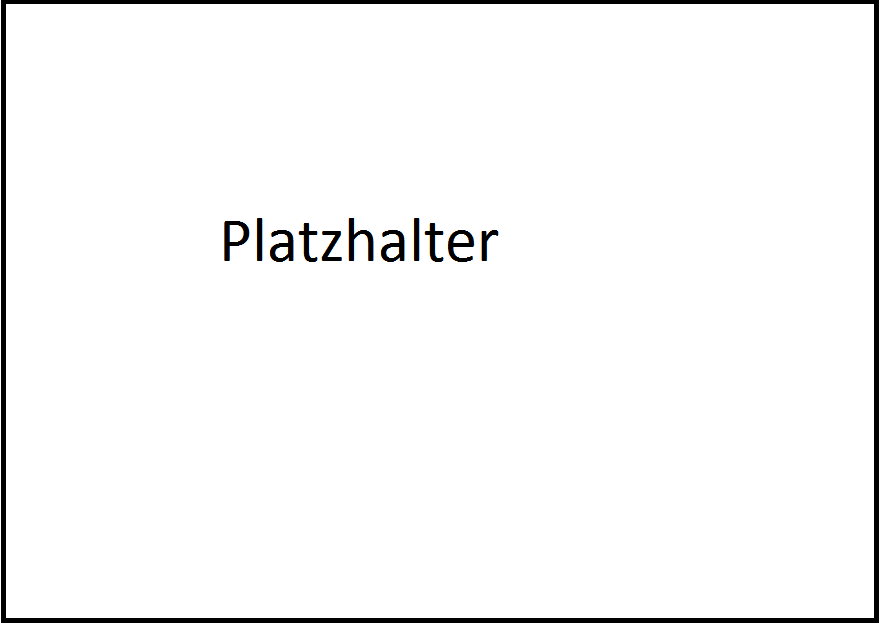
\includegraphics[width=\textwidth]{img/00_placeholder.png}
%      
\end{figure}

Aus der Abbildung~\ref{fig:wavenumber_wavelength} lässt sich folgender Zusammenhang ableiten.
%
\begin{equation}
\label{eq:Phase_Wavenumber}
	d(\Theta, n)=\lambda(\Theta+n)
\end{equation}

\lipsum[1]

%
%
%-----------------------------------------------------------------------
%
\section[Technische Voraussetzungen]{Technisch-Physikalische Voraussetzungen}
%
%-----------------------------------------------------
In diesem Abschnitt werden die technischen und physikalischen Grundlagen für diese Arbeit vorgestellt und das Wichtigste erörtert. Es wird auf die Besonderheiten und Merkmale des auf Funk basierenden RFID-Verfahrens eingegangen. Die andere Trackingverfahren werden, aufgrund der Unterschiedlichkeit der Systeme wird im Rahmen dieser Arbeit nicht weiter behandelt. Es kann nicht im vollem Umfang auf die Details der Technik eingegangen werden ohne den Rahmen dieser Arbeit zu sprengen. Interessierte sei die referenzierte Literatur für eine weite Lektüre empfohlen.\\
%
%
\subsection{Positionsgenauigkeit auf Funk basierender Verfahren}
\label{sec:RFID_Accuracy}
Die Positionsgenauigkeit eines auf EM basierenden Systems ist von dem Messprinzip abhängig. Dabei bieten sich im Wesentlichen drei Möglichkeiten:\\
%
\begin{table} [ht!]
	\begin{center}
		\begin{tabular}{lp{65mm}p{15mm}}
		1. & Laufzeitmessiung & \textbf{TOA} \\
		2. & Messung der Signalsträrke & \textbf{RSSI} \\
		3. & Phasendifferenzmessung & \textbf{PD} \\
		\end{tabular}
	\end{center}
\end{table}
%
Eine Laufzeitmessung des Signals kommt aufgrund der Ausbreitungsgeschwindigkeit der EM-Welle nicht in Frage, da diese typischerweise gleich der Lichtgeschwindigkeit ist und die Distanz zwischen Sender und Empfänger zu gering ist. Das reduziert die Möglichkeiten auf zwei Verfahren.
Bei der RSSI wird die Stärke des empfangenen Signals ausgewertet. Dies stellt eine einfache Art der Positionsermittelung dar. Jedoch kann die Signalstärke stark schwanken und erlaubt nur eine geringe Ortsauflösung.
Bei der PD wird die Postion anhand der zurückgestrahlten Welle ermittelt, genauer der Phase der Welle.

\subsection{RFID}
%
Bei \textit{Radio-Frequency Identification} (RFID) handelt es sich um einen Funkstandard der die kontaktlose Identifikation bei gleichzeitiger Erfassung zusätzlicher Informationen ermöglicht (Payload). Zur Technik gehört ein Auslesegerät (Reader) und ein oder mehrere Transponder (Tags). Eine sehr grobe Übersicht über typische Bauformen von Tags und Reader ist in \ref{fig:RFID_TAGS_AND_READER} zu finden. Die dargestellten Tags sind für verschiedene Frequenzbänder. Heute verfügbare Transponder lasen sich auf nahezu jeder beliebigen Oberfläche anbringen. Das ermöglicht ein großes Anwendungsspekrum, praktisch wird die Technik in jeder Umgebung eingesetzt in der es erforderlich oder nützlich ist, Dinge kontaktlos zu identifizieren. Eine gute Übersicht über Branchen und Anwendungsgebiete für RFID ist in \cite{RFIDJournal} zu finden. Im Rahmen dieser Arbeit wird kein umfassender Überblick über die Technik geboten, da die Bauformen und Spezifikationen sehr stark variieren. Ein Umfassendes Werk, gute Einführung und Übersicht zur Technik bietet~\cite{finkenzeller2008rfid}. Dort werden auch detailliert die physikalischen Grundlagen verschiedener Antennenbauformen und Tags erläutert. Aufgrund des großen Anwendungsspektrums und der weiten Verbreitung ist die Technik in die Kritik geraten. Unter dem Dach des Vereins \textit{digitalcourage e.V.} existiert die Kampange \textit{StopRFID}. Die Kampagne hat sich zum Thema gemacht über die Anwendungsmöglichkeiten und Risiken von RFID aufzuklären \cite{stoprfid2013}. Die Seiten der Kampagne bieten eine sehr weitgehende Auflistung der Anwendungen für RFID.\\
%Ziel der Kampagne ist es die Gefahren in den gesellschaftlichen Fokus zu rücken und für den Umgang mit der allgegenwärtigen Technik zu sensibilisieren. Die Kampagne über sich selbst:
%\begin{quote}
%"Wir wollen RFID nicht komplett verhindern. Es geht uns nicht darum, die RFID-Entwicklung zum Erliegen zu bringen ... Im Gegenteil." \footnote{\url{http://www.foebud.org/rfid/was-kann-ich-tun/}}
%\end{quote}
%
\begin{figure} [h!]
\centering
         \caption[Beispiele für Transponder und Lesegeräte]{ Hier gezeigt sind Beispiele für RFID Transponder und Lesegeräte. Das linke Bild zeigt drei typische Tags, nahezu jede Gestalt ist mittlerweile erhältlich. Die hier gezeigten Tags eignen sich für eine Anbringung an glatten Oberflächen. Es gibt zig weitere Bauformen, die unterschiedlichste Anwendungsspektren bedienen und sogar eine Implantation ermöglichen (nicht gezeigt). Im rechten Bild ist ein Handlesegerät gezeigt. Zum Mobilen Auslesen über mittlere bis kurze Distanzen. Auch bei den Readern gibt es unterschiedlichste Bauformen, die je nach Anwendungsfall ausgewählt werden.}
         \label{fig:RFID_TAGS_AND_READER}
         \vspace{0.5cm}%         
         \begin{subfigure}[h]{0.4\textwidth}
                 \centering
                 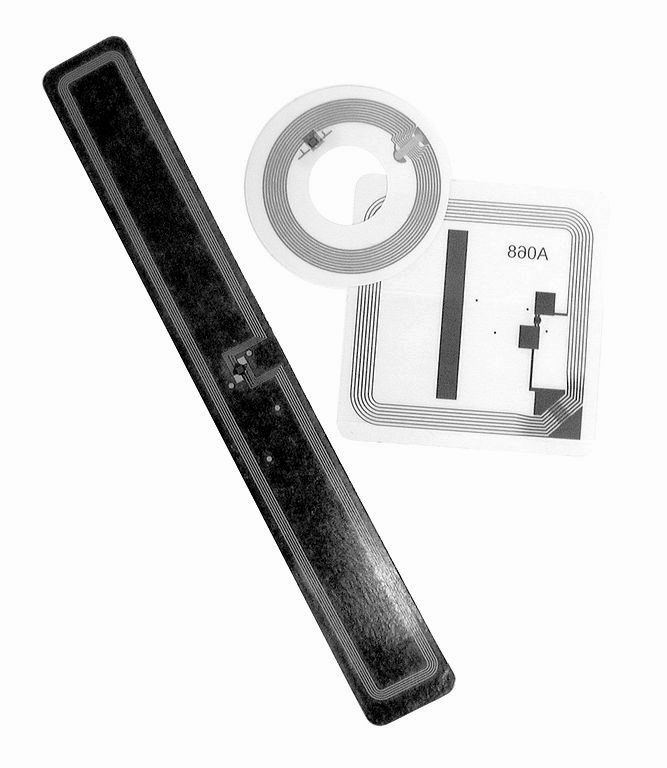
\includegraphics[width=\textwidth]{img/667px-RFID_Tags_gs.png}
                 \vspace{.1cm}
                 \caption{ RFID- Transponder}
                 \label{fig:TAGS}
         \end{subfigure}
%         
\qquad
%
         \begin{subfigure}[h]{0.4\textwidth}
                 \centering
                 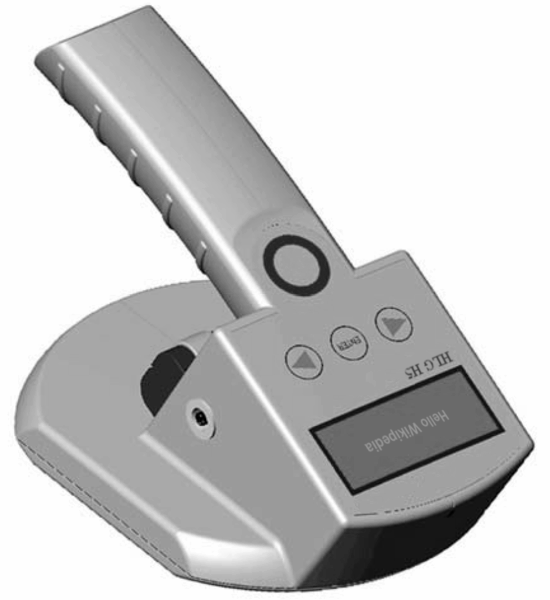
\includegraphics[width=\textwidth]{img/RFID-Reader_gs.png}
                 \vspace{.1cm}
                 \caption{RFID- Handlesegerät }
                 \label{fig:READER}
         \end{subfigure}
\end{figure}
%
\label{sec:Measurement1}
%
%

Die Messung der Position erfolgt über die Auswertung der Phasenlage des empfangenen Signals in Bezug auf ein Referenzsignal. In der EU gibt es verschiedene zulässige RFID-Frequenzen sie reichen von $865,0$ MHz bis $868,0$ MHz~\cite{etsi1}. Man kann man die Wellenlänge mit: $ \lambda\simeq0,35 m $ angeben. Daraus folgt, dass alle 35 cm die gleiche Konfiguration der Phase vorliegt. Im Rahmen dieser Arbeit wird dabei von \textit{Isophasen} gesprochen. Daraus folgt, dass die gewonnene Information aus der Phase ist nicht eindeutig ist. D.h. es lässt sich durch die Kenntnis der Phase nicht unmittelbar auf die korrekte Postion des Tags schließen. Man kann das Problem umgehen in dem man auf die errechnete Position ein ganzzahliges Vielfaches der Wellenlänge addiert, siehe Gleichung~\ref{eq:Phase_Wavenumber}. Die dort beschriebene Konstante $n$ wird Wellenzahl genannt.\\
%

Das System der Amedo STS verwendet eine spezielle Antennenanordnung um die Position zu ermitteln. Dabei wird eine Antennenanzahl >4 eingesetzt. Für jede dieser Antennen muss eine eigene Wellenzahl bestimmt werden. Durch Auslöschung des Signals, Absorption etc. kann es dazu kommen, dass eine Antenne eine unbestimmte Zeit lang kein Signal vom Tag empfängt. Wenn die Antenne nach dieser Zeit erneut ein Signal empfängt ist die ihr zugehörige Wellenzahl unbekannt und muss neu bestimmt werden. \\
%

In realen Umgebungen treten zusätzlich noch Reflektionen und ein sog. Multipath-Effekt auf. Dabei wird das Signal nicht auf dem Direkten Weg Antenne-Tag-Antenne empfangen sondern über einen unbekannten, längeren Weg. Dadurch kommt es zu einem Fehler in der Phase. Zusätzlich ist dieser Effekt individuell für jede Antenne.
%

\subsection{PRPS-Messystem}
%
\begin{floatingfigure}[hr!]{7cm}
         \centering
         \caption[PRPS der \amedogmbh]{Abgebildet ist der Messaufbau aus vier Antennen. In dem Aufbau verbaut sind die wesentlichen elektronischen Komponenten wie Auswerte- und Steuereinheit. Nicht einzeln gezeigt.}
         \vspace{2mm}
         \label{fig:System}
         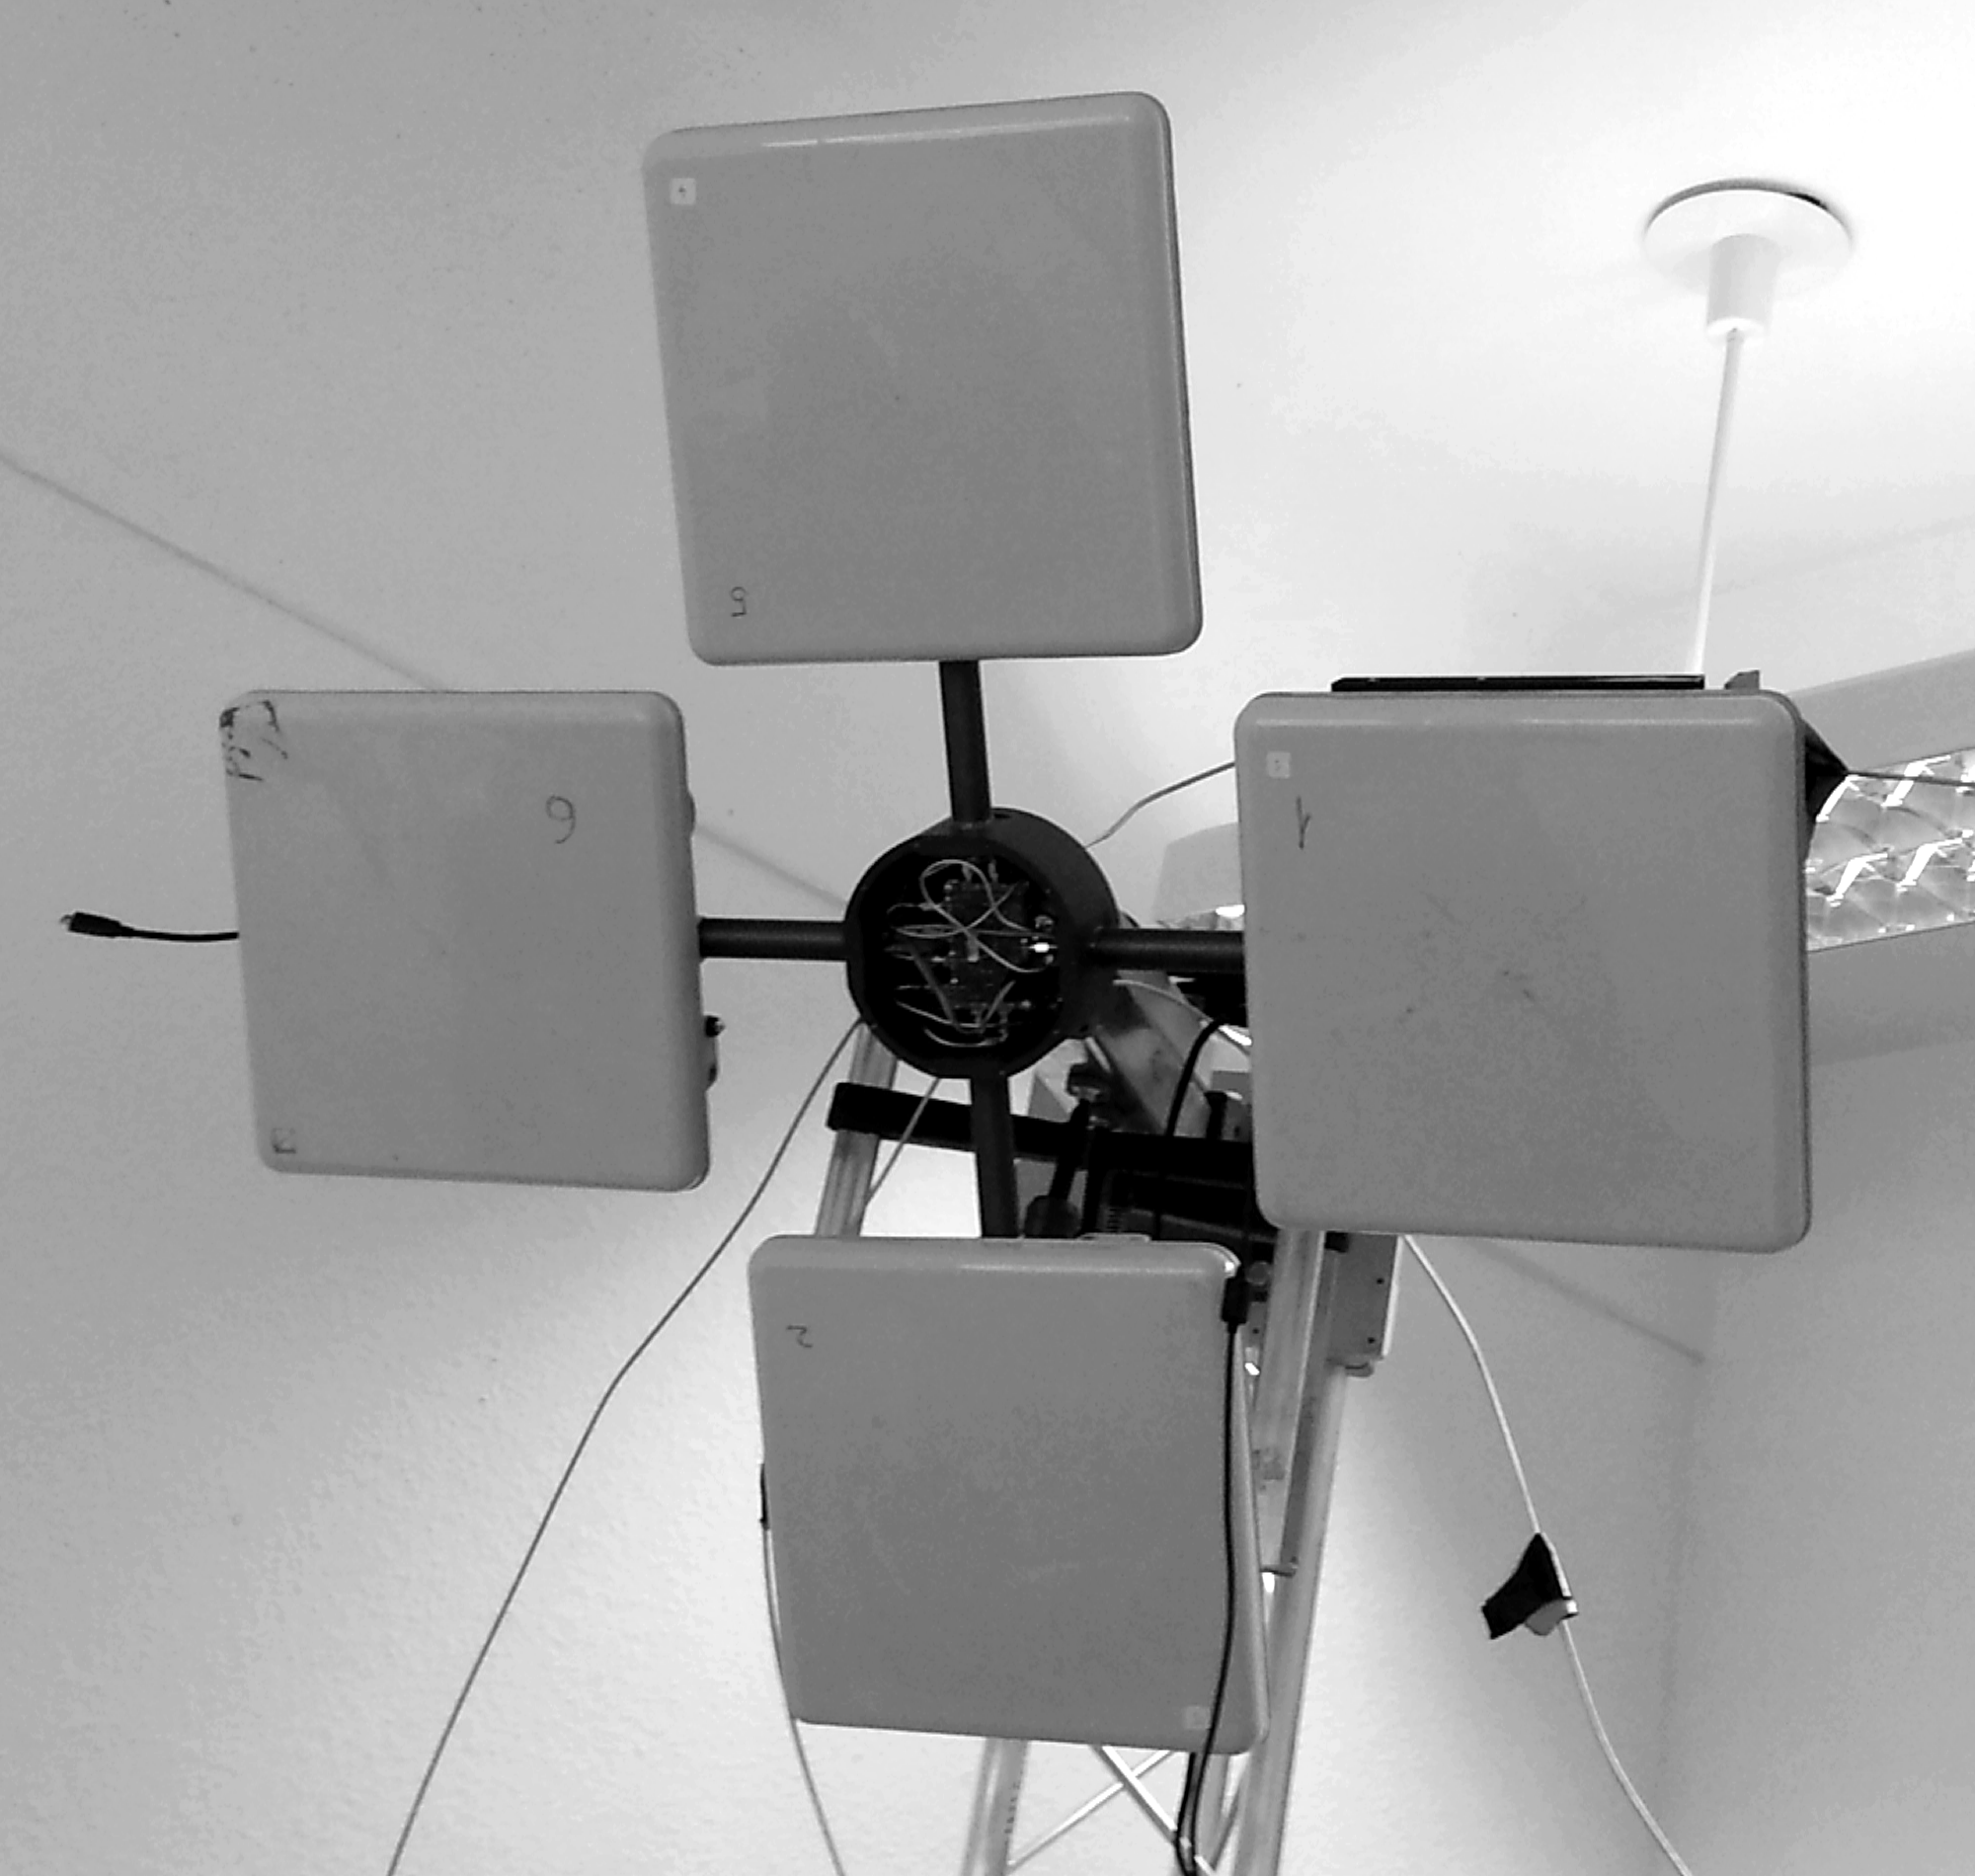
\includegraphics[width=0.4\textwidth]{img/4AntennaSetup_small.png}
         \vspace{2mm}
%         
\end{floatingfigure}
%
Diese Arbeit wird für das Messsystem der \amedogmbh entwickelt. Die Entwicklung wird Teil der Softwarekomponenten des Systems werden. Aktuelle befindet sich das gesamte System in der Revision, in diesem Abschnitt wird der Stand der Entwicklung dargestellt. Details über Hardware und Software werden im Rahmen der Arbeit nicht besprochen, sofern sie diese Arbeit nicht unmittelbar betreffen. \\
%

Das auf RFID basierende PRPS (Passiv RFID Positioning System) besteht aus mehreren frei positionierbaren Antennen. Eine Mess- und Steuereinheit sowie einem Rechner zur Kommunikation mit Endkundensoftware. Die Systemkomponenten für die Messwertaufnahme und Steuerung sind in einem Gehäuse untergebracht, dieses zeigt Abbildung~\ref{fig:System}. Eine typische Installation ist in Abbildung~\ref{fig:Setup} gezeigt. Dort wurde ein System mit insgesamt acht Antennen installiert. Vier Antennen sind frei aufgestellt, vier Weitere in einer festen Anordnung (\textit{Spinne}) installiert. Der Aufbau ist auf ein Messvolumina gerichtet.\\
%
\subsubsection{Leistungsmerkmale}
%
Das PRPS erlaubt eine Identifikation mehrerer Objekte oder genauer: RFID-Tags die auf den Objekten angebracht sind. Wird ein einzelner Tag ausgewählt kann seine Postion mit einer einer sehr hohen Frequenz ausgegeben werden. Die momentan Erreichbare Werte liegen bei $60$~Hz. Je nach Umgebung kann dieser Wert jedoch Variieren, siehe Kapitel~\ref{sec:Komplexity1}. Sollen mehrere Tags ausgegeben werden, verringert sich die Frequenz entsprechend. Bei der Verwendung von drei Tags ist einer Leserate von $20$~Hz pro Tag realistisch. Die Positionsgenauigkeit liegt aktuell bei $\approxeq 5$~mm. Die Antennen können frei Arrangiert werden. Das erlaubt eine Anpassung an nahezu jeden Raum und jeden Kundenbedarf. Als Tags kommen jeder Handelsübliche RFID-Tag im verwendeten Frequenzband im Bereicht der ETSI-Frequenzen~\cite{etsi1} in Frage. Der Messbereich liegt bei mehreren Kubikmetern und einer erprobten maximalen Entfernung von $6-7$~Metern. Theoretisch ist das maximale Volumen noch größer. Die leistungstarke Messeinheit besteht aus einer sehr flexiblen Messelektronik. Diese ist in der Lage eine sehr hohe Güte und Frequenz der Messwerte zu realisieren.\\

%
\begin{figure}[h]
         \centering
         \caption[Messaufbau der Amedo GmbH]{Abgebildet ist der Messaufbau mit unterschiedlichen Antennen. Der Aufbau ist auf ein Messvolumina von mehreren Kubikmetern ausgerichtet}
		\label{fig:Setup}
		\vspace{2mm}
         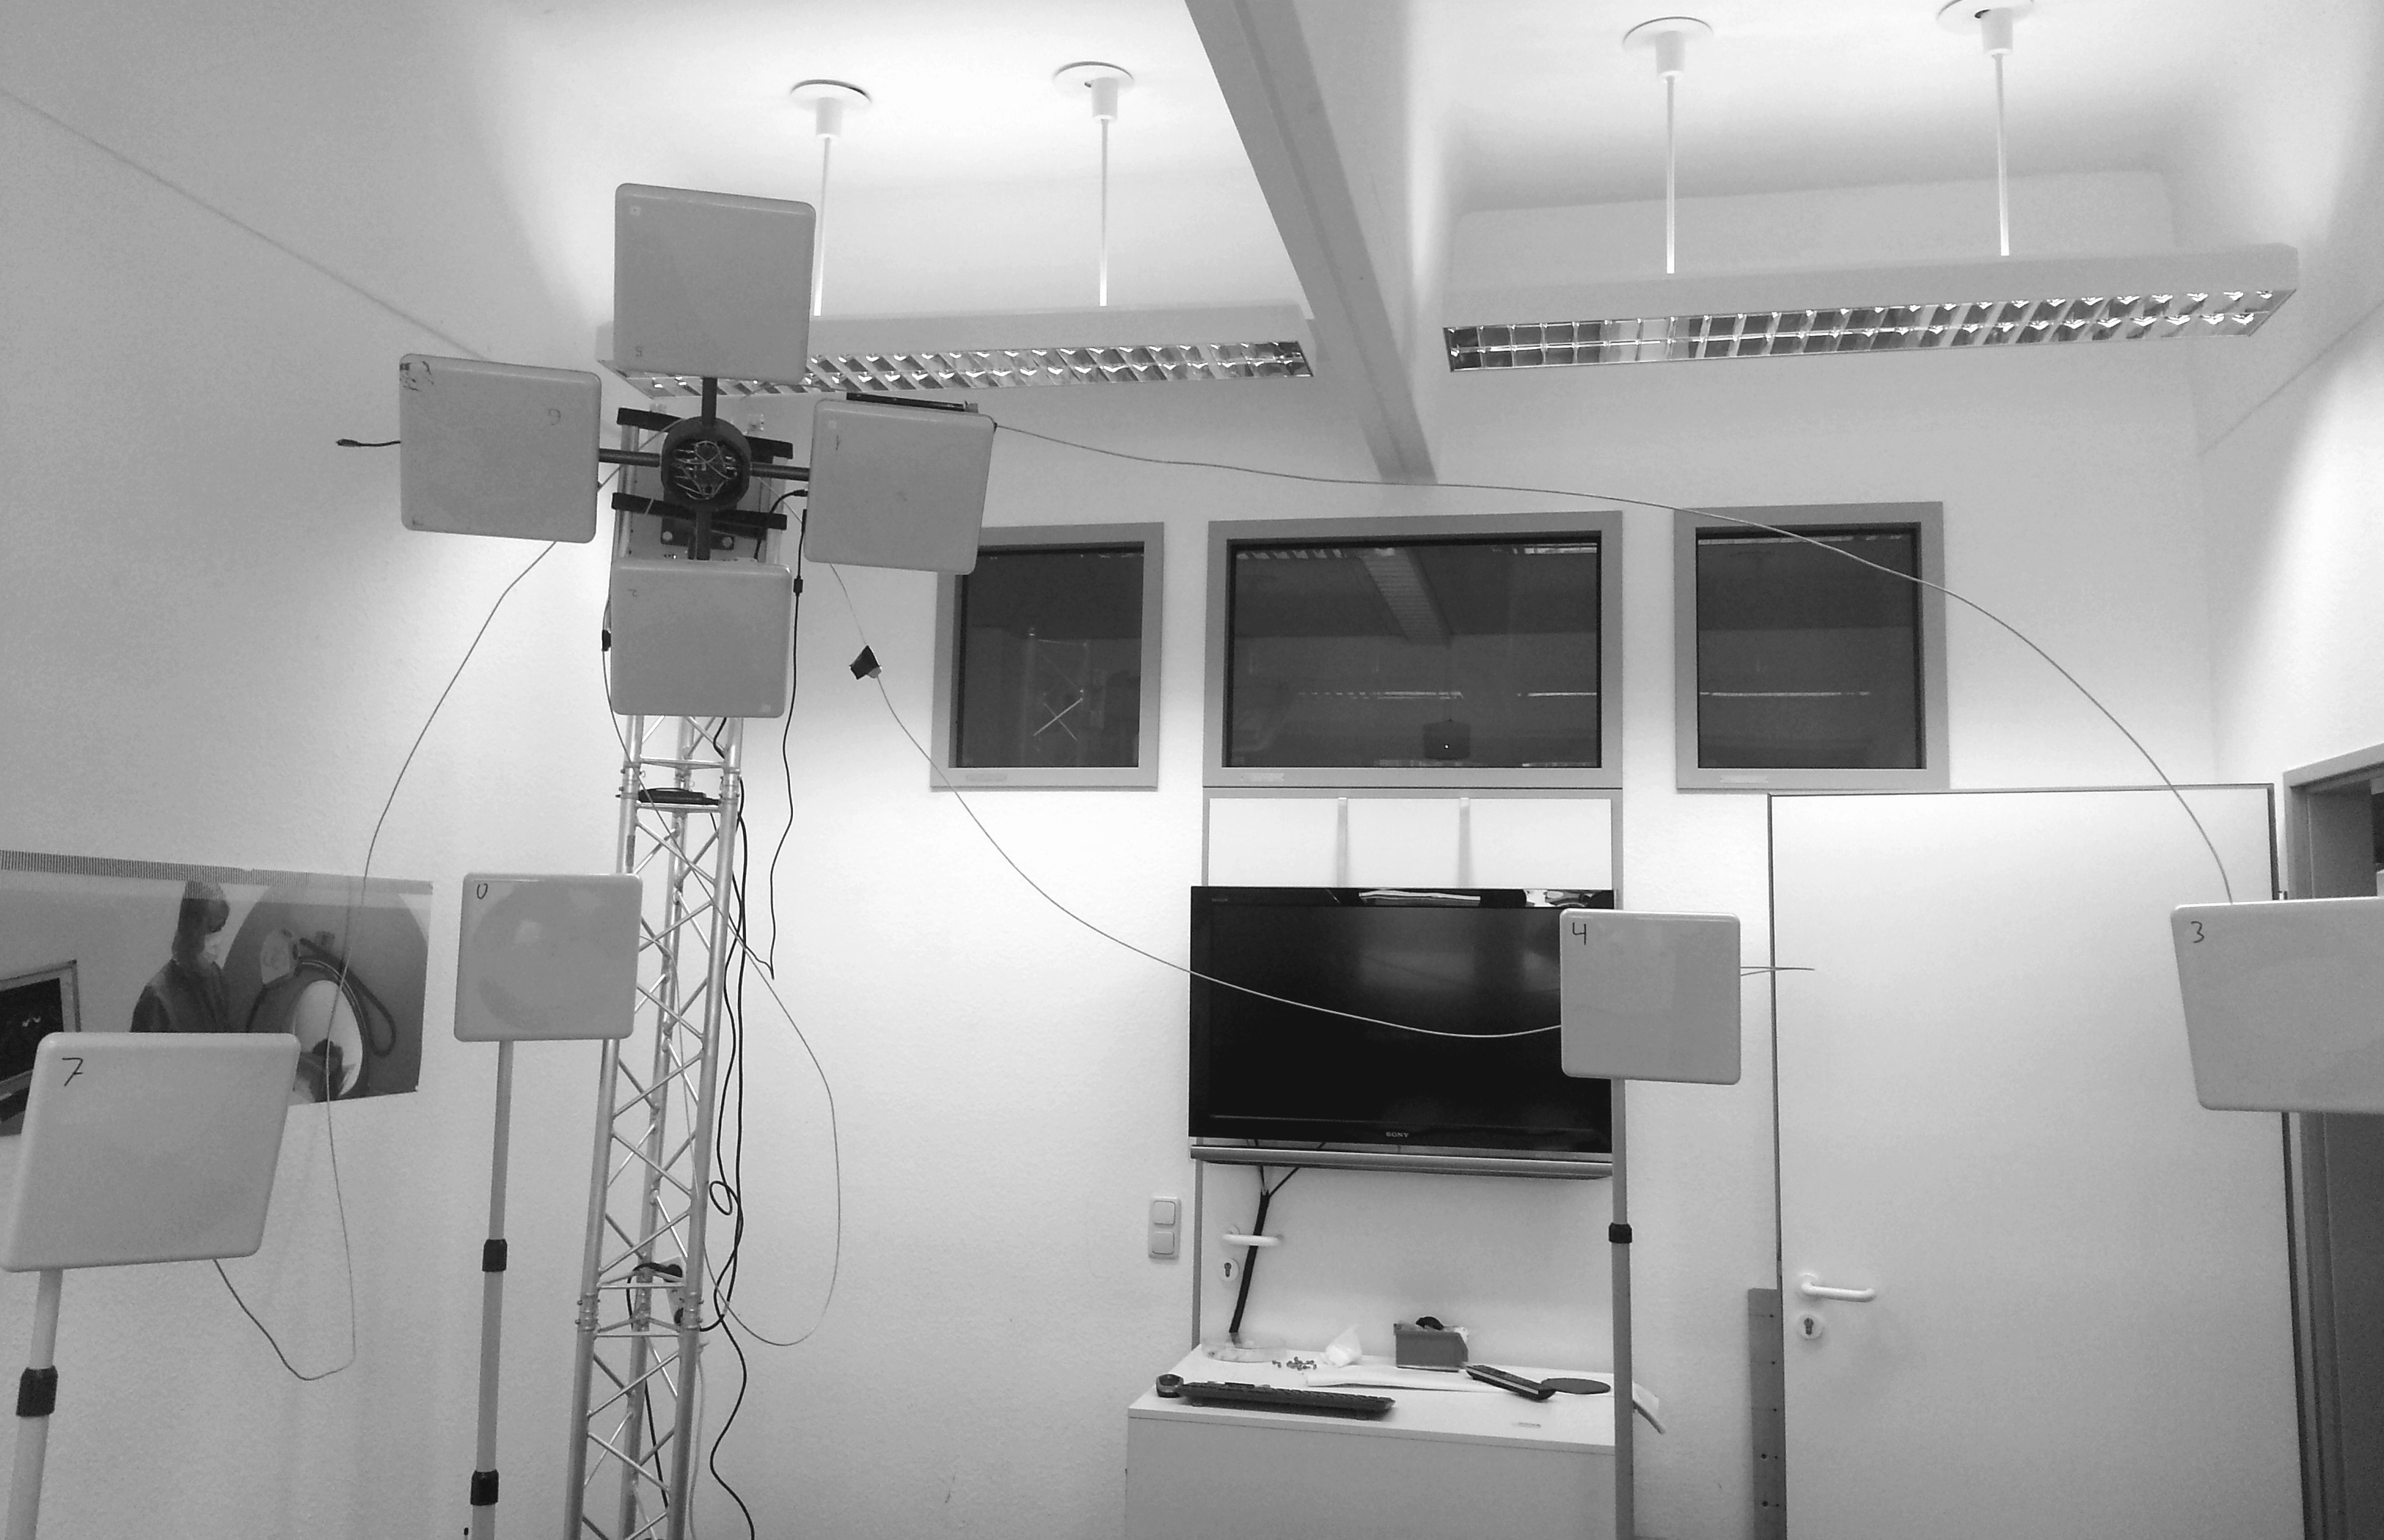
\includegraphics[width=\textwidth]{img/RFID-Okto.png}
         
\end{figure}
%
%-----------------------------------------------------------------------

%

% 2. ------------------------------------------------------------------------
\chapter{Hauptteil}
Im Folgenden werden ausführlich die Methoden und Lösungen zur beschriebenen Problemstellung vorgestellt. Zuerst wird eine Betrachtung der Komplexität des Problems präsentiert. Es werden die Modelle vorgestellt die zum Auffinden der Lösung verwendet wurden. Im Anschluss wird die Implementation der ES und die Schnittstellen zum PRPS beschrieben.
%
\section{Vorüberlegung zur Komplexität}
\label{sec:Komplexity1}
%
\begin{floatingfigure}[hr!]{6cm}
 \centering
         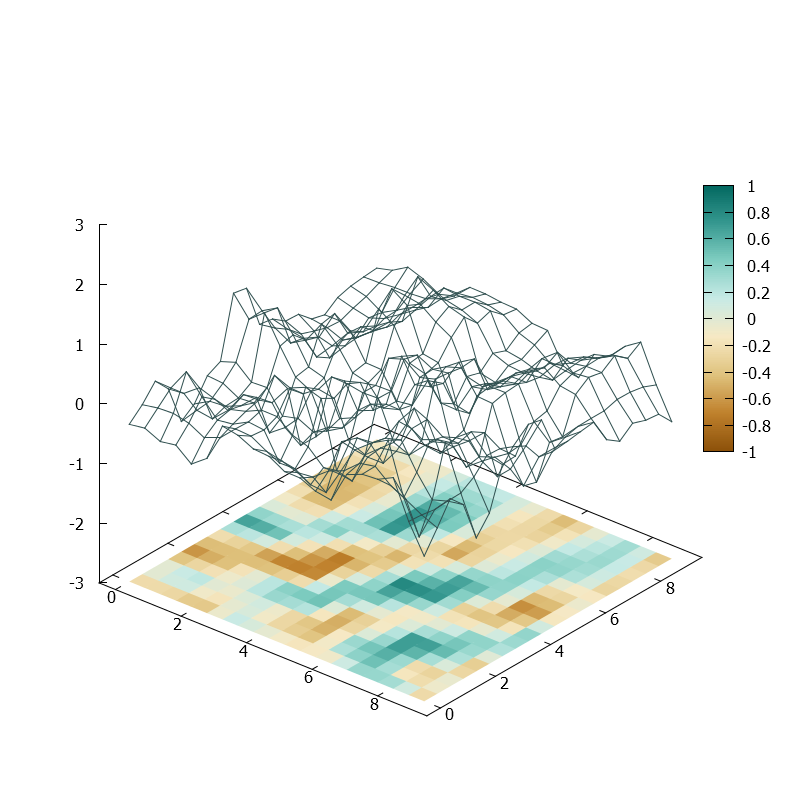
\includegraphics[width=7cm]{img/Plate0_A1.png}
         \caption[Profil einer Phasenmessung]{Normiertes Höhenprofil einer Phasenmessung aus der Sicht von Antenne 1 }
         \label{fig:Plate0_A1_}
\end{floatingfigure}
%
In diesem Abschnitt wird eine Übersicht über die Komplexität des Problems gegeben. In der rechten Abbildung zu sehen ist vergrößert Visualisierung einer typischen Kalibriermessung. Der verwendete Aufbau ist in Abbildung~\ref{fig:Spider1}. gezeigt. Er besteht aus vier Antennen die in einer Ebene angeordnet sind. Es wurde eine reproduzierbare Aufstellung verwendet (Abbildung~\ref{fig:Spider_setup1}) und eine Fläche von $1\times1$ Meter vermessen. Alle $10$ cm wurde eine Messung gespeichert. In der Abbildung kann man deutlich das Verhalten der Phasendaten sehen. Um diesen Verlauf deutlicher zu zeigen wurden die Phasenwerte normiert und als Oberfläche in den Plot gelegt. Am Boden gezeigt ist der Kontur-Plot der Werte. Zwischen den Werten wurde Interpoliert um die Nulldurchgänge deutlicher zu zeigen. Die Übersicht aus der Sicht aller Antennen ist in Abbildung~\ref{fig:Real_Measurements} gezeigt.\\
%

In der Abbildung~\ref{fig:Complexity1} werden die Daten ohne Interpolation dargestellt. Es wurden die Höhenlinien eingezeichnet. Die Anordnung der Plots soll ein Gefühl dafür vermitteln, wie die Messwerte eines Tags sich an unterschiedlichen Postionen und aus sich verschiedener Antennen verhalten.\\
%

Die Darstellung echter Messwerte lässt Rückschlüsse auf die Komplexität des Problems zu. Es ist leicht nachzuvollziehen, dass das Zusammenspiel der Messwerte eine sehr komplexe Szene ergibt. Hier dargestellt ist bereits das Verhalten bei der Verwendung von vier Antennen. Der aktuelle Messaufbau erlaubt sogar acht Antennen. Das ergibt insgesamt eine komplexe Szenerie.\\
%
\begin{figure}[ht!]
        \centering
        \begin{subfigure}[b]{0.4\textwidth}
            \centering
            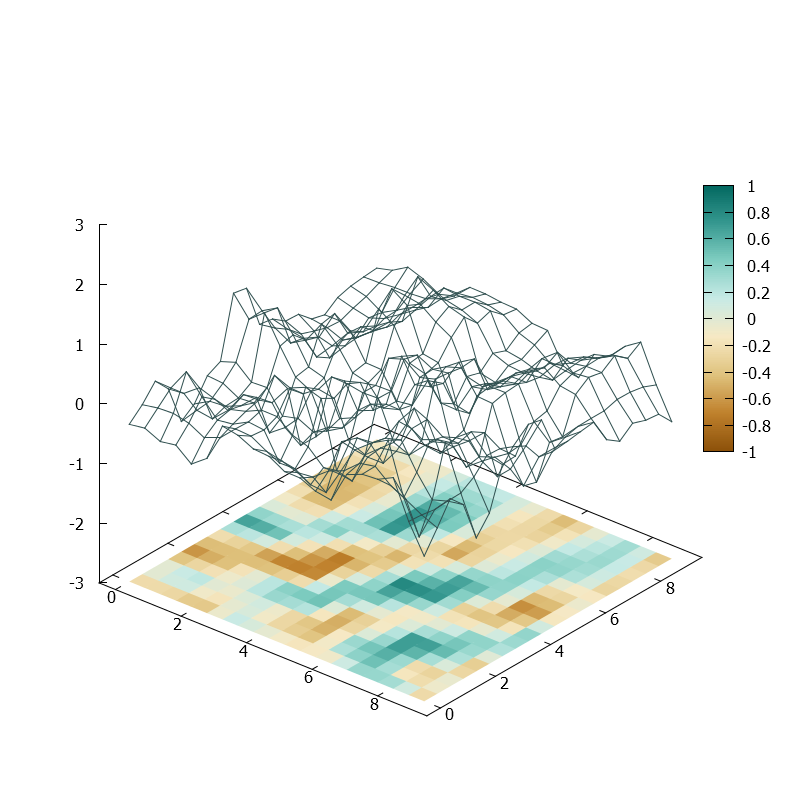
\includegraphics[width=\textwidth]{img/Plate0_A1.png}
            \caption[lorem]{Antenne 1}
            \label{fig:Plate0_A1}
        \end{subfigure}%
\\
        \begin{subfigure}[b]{0.4\textwidth}
            \centering
            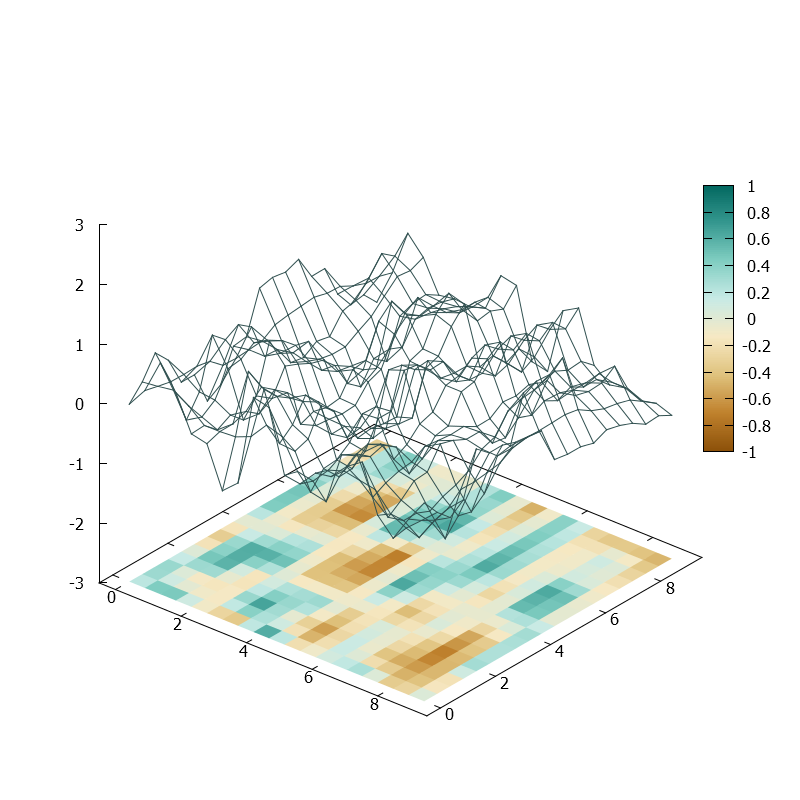
\includegraphics[width=\textwidth]{img/Plate0_A2.png}
          	\caption[Loren ipsum]{Antenne 2}
         	\label{fig:Plate0_A2}
        \end{subfigure}
\qquad\qquad
        \begin{subfigure}[b]{0.4\textwidth}
			\centering
			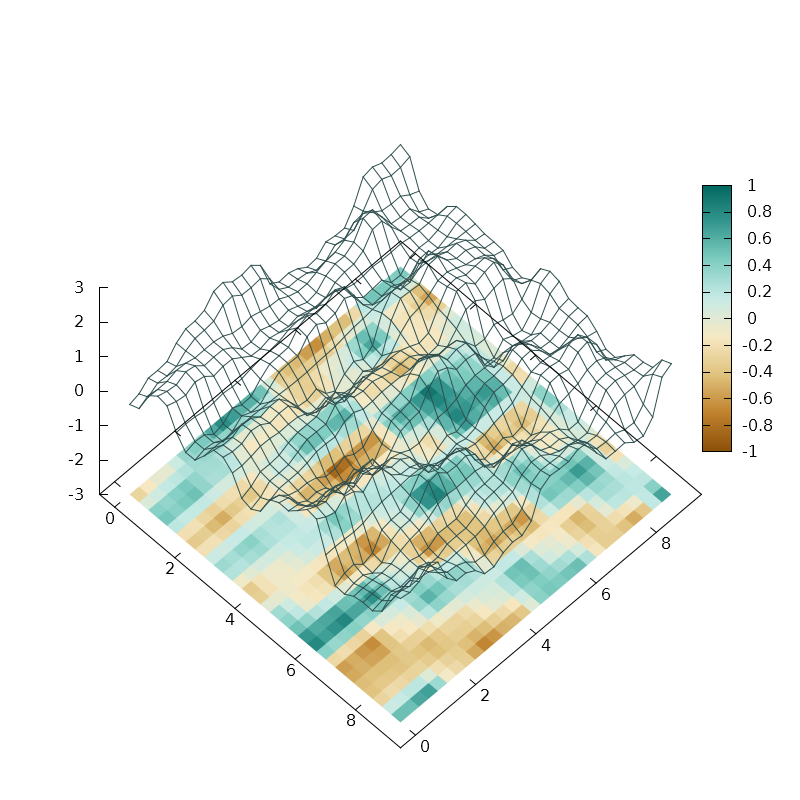
\includegraphics[width=\textwidth]{img/Plate0_A4.png}
			\caption[Loren ipsum]{Antenne 4}
			\label{fig:Plate0_A3}
        \end{subfigure}
\\
        \begin{subfigure}[b]{0.4\textwidth}
			\centering
			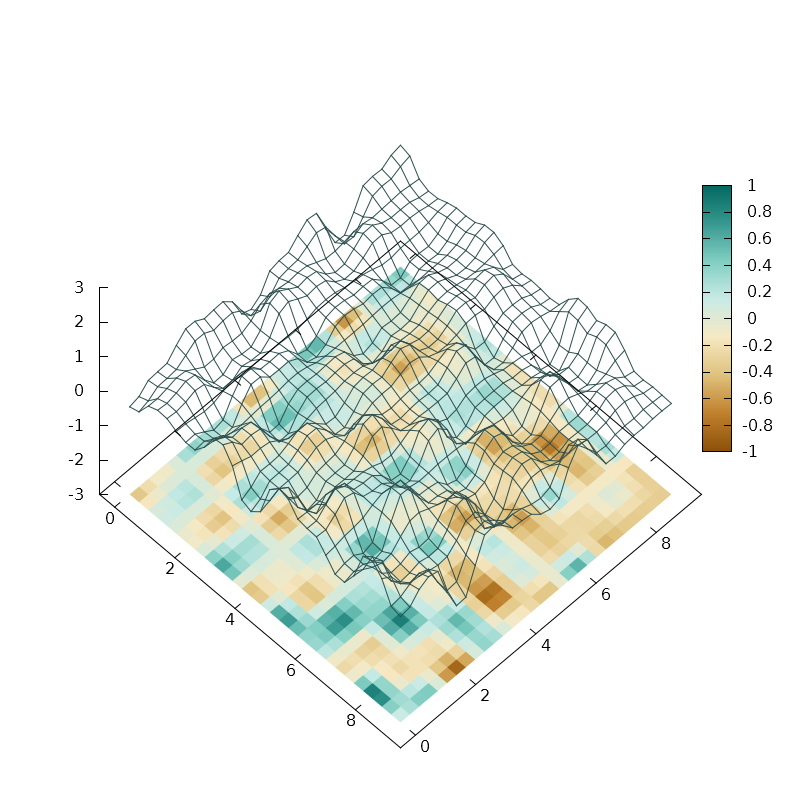
\includegraphics[width=\textwidth]{img/Plate0_A3.png}
			\caption[Loren ipsum]{Antenne 3}
			\label{fig:Plate0_A4}
        \end{subfigure}
        \caption[Reale Messwerte visualisiert]{Blick auf die Messwerte der  Kalibrierplatte aus der "Sicht" der Antennen. Dabei zeigt sich deutlich der Wellencharakter der Messung, dieser ist zu erwarten. Die Messung würden mit bei einer Frequenz von $865,7$ MHz unter Laborbedingungen aufgenommen. }\label{fig:Real_Measurements}
\end{figure}
%
\begin{figure}[ht!]
         \centering
         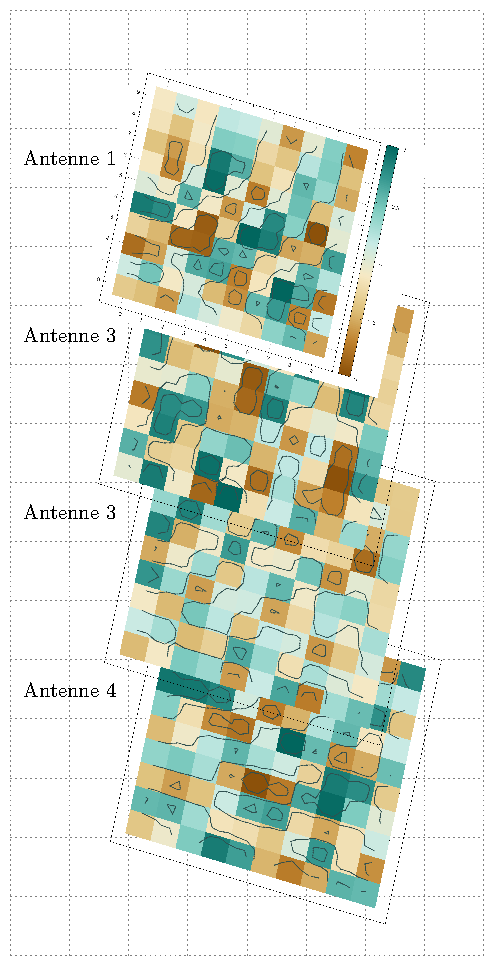
\includegraphics[width=0.6\textwidth]{img/complexitiy1.pdf}
%         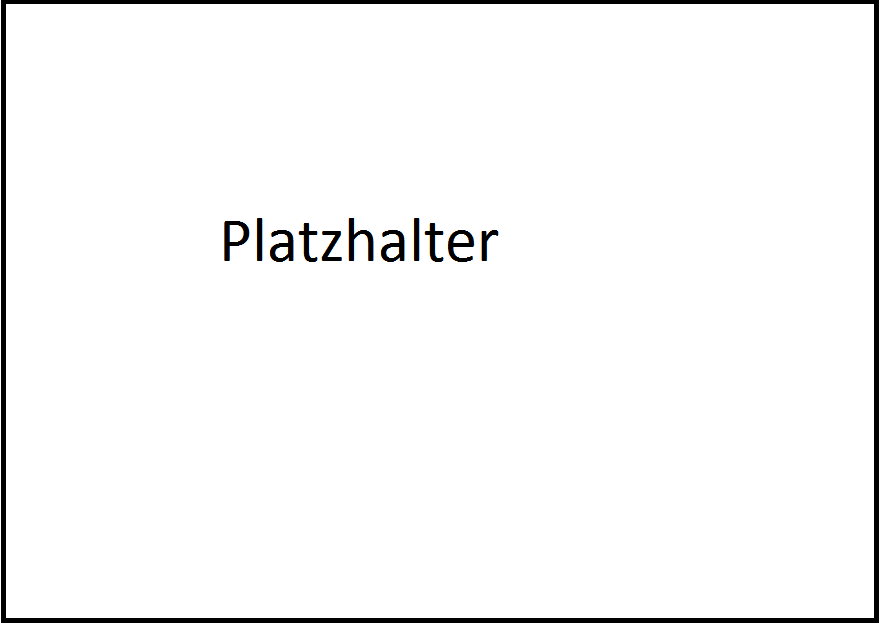
\includegraphics[width=0.7\textwidth]{img/00_placeholder.png}
         \caption[Normierte Messwerte von Kalibriermessung]{Diese Grafik zeigt die Visualisierung von realen Phasen-Messwerten. Die Daten wurden durch Vermessung einer $1\times1$-Kalibrierplatte mit reproduzierbarer Aufstellung\footnote{In dieser Arbeit nicht gezeigt} gewonnen. Die Daten wurden normiert. In jeder Dimension wurden $10\times10$ Werte aufgenommen. Die Darstellung der Phasenwerte erfolgt als Heatmap, es soll qualitativ der Verlauf der Phasenwerte gezeigt werden. Zur Orientierung sind in jedem Plot Höhenlinien eingezeichnet. Pro Plot werden die Daten einer Antenne dargestellt. Die Antenne von der die Daten stammen ist angegeben.}
         \label{fig:Complexity1}
%
\end{figure}


%
\section{Entwicklung des Modells}
\label{sec:model_developement}
Im folgenden Abschnitt wird das Modell für die Lösung des Zusammenhangs entwickelt. Zur Veranschaulichung des Sachverhalts dient die Abbildung~\ref{fig:TrilaterationScene}. Dort skizziert ist der Messaufbau mit einem Tag. Die Szene ist in 2D dargestellt die Ableitung des Modells erfolgt direkt für drei Raumkoordinaten.
%
\begin{figure}
	\begin{center}
		\caption[Antennen-Szene mit einem Tag]{2D-Übersicht auf die Szene mit drei Antennen, einem Tag und einer Landmarke. Die Position von $\{A_1,A_3,A_3\}$, sowie der Landmarke, zum Koordinatenursprung sind bekannt. Die Vektoren $r_1,r_2,r_3$ sind die gemessene Entfernung zu einer Antenne. Die Landmarke wird im späteren Verlauf eine Antenne sein, die ihrerseits ein gemessene Entfernung $r_0$ produziert. Der Schnittpunkt aller Kreise ist die Lösung der gemessenen Entfernung und der geom. Anordnung, die sich für die Position des Tags ergibt.} 
		\label{fig:TrilaterationScene}
		\input{img/trilaterationScene.tex}
%		
	\end{center}
\end{figure}
%
Folgende Nomenklatur und Symbole gelten für diesen Abschnitt:
\begin{itemize}[itemsep=0mm]
	\item	$r_{k}$ := Abstand vom Tag zur Antenne
	\item	$d_{kJ}$ := Abstand zur Landmarke
	\item	$N_0:=$ Menge der verfügbaren Antennen $N=\{1,..,8\}$
	\item	$N:=$ Menge der Antennen die für die Optimierung verwendet werden können ($N \subseteq N_0$)
	\item	$N':=$ Menge der Antennen die für die Optimierung verwendet werden ($N' \subseteq N$)
%	; Dabei ist $|N'| \geq 3$
%	\item	Es gilt $|N'| \geq |N| \geq |N_0|$   
	\item	$j$ ist der Index der Referenzantenne, es gilt $j = \{1,2,..,8\}$
	\item	$k$ ist der Index der Antennen einer Messung, es gilt $k = 1,2,..,|N'|-1$
\end{itemize}
%
Wir starten mit der Überlegung über den geometrischen Zusammenhang zwischen der Antennenposition von Antenne $k$ zu der Position des Tags $r_k$:
\begin{align}
	\label{eq:base_vactor}
	r_{k}^2 &= (x-x_k)^2+(y-y_k)^2+(z-z_k)^2
\end{align}
%
Diese Gleichung stellt die Euklidische Vektornorm dar und entspricht der Strecke Antenne-Tag. Für die Ermittelung einer Postion (mit drei Raumkoordinaten) sind drei Antennen Notwendig. Daraus ergibt sich:
%
\begin{itemize}
\item 3 Gleichunge n
\item 3 Unbekannte
\item Quadratisches Gleichungssystem
\end{itemize}
%
Das Gleichungssystem sieht wie folgt aus:
%
\begin{align}
	r_{1}^2 &= (x-x_1)^2+(y-y_1)^2+(z-z_1)^2 \nonumber\\
	r_{2}^2 &= (x-x_2)^2+(y-y_2)^2+(z-z_2)^2 \nonumber\\
	r_{3}^2 &= (x-x_3)^2+(y-y_3)^2+(z-z_3)^2 \nonumber
%	
\end{align}
%
Es ist trivial und wird in verschiedenen Beispielen gezeigt\footnote{z.B. \url{http://en.wikipedia.org/w/index.php?title=Trilateration&oldid=553215995}}, dass man die Koordinaten aus dem quadratischen Gleichungssystem unmittelbar berechnen kann. Es muss jedoch ein quadratisches Gleichungssystem gelöst werden, was zu den bekannten Problematiken führt, insbesondere der Ausschluss mehrdeutiger Ergebnisse. Der Messaufbau der \amedogmbh erlaubt die Verwendung von mehr als 3 Messwertgebern. Diese zusätzliche Informationen lassen sich für eine Linearisierung des Gleichungssystems verwenden. Dieser Ansatz wird für ein Modell im Rahmen dieser Arbeit verwendet und wird im Folgenden beschrieben.\\
%
Von den Antennen sind die Raumkoordinaten ($x,y,z-Koordinaten$) bekannt, bzw. wurden durch Kalibrierung \ref{sec:calibration} in einem vorherigen Schritt bestimmt. Wir können zusätzlich zu notieren:
%
\begin{equation}\label{eq:d_k0}
	d_{kj}^2= (x_k-x_0)^2+(y_k-y_0)^2+(z_k-z_0)^2
\end{equation}
%
Linearisierung des Modells. Dazu wird Gleichung~\ref{eq:base_vactor} in mehreren Schritten umgebaut. Zuerst wird eine neutrale Erweiterung durchgeführt und die Terme geschickt zusammengefasst. Das führt zu:
%
\begin{align}
	r_{k}^2 &= (x-x_k)^2+(y-y_k)^2+(z-z_k)^2 \nonumber \\
	&=(x-x_k+x_0-x_0)^2+(y-y_k+y_0-y_0)^2+(z-z_k+z_0-z_0)^2 \nonumber \\
	&=((x-x_0)-(x_k-x_0))^2+((y-y_0)-(y_k-y_0))^2+((z-z_0)-(z_k-z_0))^2 \nonumber \\ 
	%2 bin. Form
	&=(x-x_0)^2-2(x-x_0)(x_k-x_0)+(x_k-x_0)^2\underbrace{+\dots{}+\dots{}}_\text{y-\& z-Terme analog}
	\label{eq:tri_temp1}
%
\end{align}
%
Um Platz zu sparen sind die y- und z-Terme nicht explizit notiert. Sie ergeben sich durch einfaches Ersetzen der Indizes und werden im Finalen Modell eingefügt. Durch Umstellen von \eqref{eq:tri_temp1} erhalten wir:
\begin{align}
(x-x_0)(x_k-x_0)+\dots{}+\dots{}&=-\frac{1}{2}[r_k^2-(x_k-x_0)^2 -(x-x_0)^2 +\dots{} +\dots{}]\nonumber\\
(x-x_0)(x_k-x_0)+\dots{}+\dots{}&=\phantom{-}\frac{1}{2}[(x_k-x_0)^2 +(x-x_0)^2 +\dots{}+\dots{}-r_k^2]\nonumber
%
\end{align}
%
\begin{multline}\label{eq:rk_final}
(x-x_0)(x_k-x_0)+(y-y_0)(y_k-y_0)+(z-z_0)(z_k-z_0)= \\\frac{1}{2}[(x_k-x_0)^2+(x-x_0)^2-(y_k-y_0)^2+(y-y_0)^2
\\-(z_k-z_0)^2 +(z-z_0)^2-r_k^2]
\end{multline}
%
Vergleich von \eqref{eq:rk_final} mit \eqref{eq:d_k0} bringt: 
%
\begin{multline}
(x-x_0)(x_k-x_0)+(y-y_0)(y_k-y_0)+(z-z_0)(z_k-z_0)= \\\frac{1}{2}[\underbrace{(x_k-x_0)^2+(z_k-z_0)^2+(y_k-y_0)^2}_\text{\boldmath{$d_{kj}^2$}}
\\+\underbrace{(x-x_0)^2+(y-y_0)^2 +(z-z_0)^2}_\text{\boldmath{$r_j^2$}}-r_k^2]
\end{multline}
%
\begin{equation}
(x-x_0)(x_k-x_0)+(y-y_0)(y_k-y_0)+(z-z_0)(z_k-z_0)=\frac{1}{2}[d_{kj}^2+r_{j}^2-r_k^2]\label{eq:rk_final_simplyfied}
\end{equation}
mit 
\begin{equation}\label{eq:c_kj}
\mathbf{c_{kj}}=\frac{1}{2}[d_{kj}^2+r_{j}^2-r_k^2]
\end{equation}
können wir das lineare Gleichungssystem abschließend schreiben:
%
\begin{equation}
%\label{eq:final_trilateration_model}
\mathbf{0}=
\left(
	\begin{array}{ccc}
		x_1-x_j & y_1-y_j & z_1-z_j \\
		x_2-x_j & y_2-y_j & z_2-z_j \\
		x_3-x_j & y_3-y_j & z_3-z_j
	\end{array}
\right)
\left(
   \begin{array}{c}
	   x-x_j\\
	   y-y_j\\
	   z-z_j
   \end{array}
\right)
-
\left(
	\begin{array}{c}
		c_{1j}\\
		c_{2j}\\
		c_{3j}
	\end{array}
\right)
\end{equation}
%
Das Gleichungssystem entspricht ist linear und hat die allg. Form: $\mathbf{0} = \mathbf{Ax}+\mathbf{b}$ es lässt sich mit bekannten Methoden lösen.




{
\small
Folgende Nomenklatur und Symbole gelten für diesen Abschnitt:
%
Wie gezeigt werden konnte\footnote{Wochenbericht KW 20, Anhang B} ergibt sich für den Fall der Trilateration und der Annahme, dass vier Antennen Messwerte liefern, die Gleichung:
\begin{equation}\label{eq:final_trilateration_model}
0=
\left(
	\begin{array}{ccc}
		x_k-x_0 & y_k-y_0 & z_k-z_0 
	\end{array}
\right)
\left(
   \begin{array}{c}
	   x-x_0\\
	   y-y_0\\
	   z-z_0
   \end{array}
\right)
-
\left(
	\begin{array}{c}
		c_{kj}
	\end{array}
\right) 
\end{equation}
%
Dabei ist:
\begin{equation}\label{eq:c_kj}
	c_{kj}=\frac{1}{2}[d_{kj}^2+r_{j}^2-r_k^2]
\end{equation}
%
Ziel dieser Erweiterung ist es, einen Zusammenhang zwischen diesem Modell und der Wellenzahl zu erzeugen. Folgender Ansatz wird gewählt:
	\begin{equation}\label{eq:r_0_varrho} r(\varrho)=\frac{\lambda}{2}\left(\frac{\varrho}{2\pi}+n\right),\\\lambda=\frac{c}{f}, n:= \text{Wellenzahl}
\end{equation}
%
%
Weiterhin ist $\varrho$ die gemessene Phase, die das PRPS-System liefert und $n$ die gesuchte Wellenzahl.\\
Durch einsetzen von \eqref{eq:r_0_varrho} in \eqref{eq:c_kj}, erhalten wir:
\begin{equation}\label{eq:c_k0_extended}
	c_{kj}(\varrho_0, \varrho_k, n_0, n_k) =\frac{1}{2}\left[d_{kj}^2+\frac{\lambda^2}{4}\left(\frac{\varrho_j}{2\pi}+n_0\right)^2-\frac{\lambda^2}{4}\left(\frac{\varrho_k}{2\pi}+n_k\right)^2\right]
\end{equation}
%
Wir stellen Gleichung~\eqref{eq:c_k0_extended} um:
\begin{align}
%	
	c_{kj}(\varrho_0, \varrho_k, n_0, n_k) &= \frac{1}{2}\left\{d_{kj}^2+\frac{\lambda^2}{4}\left[\left(\frac{\varrho_j}{2\pi}\right)^2+2\frac{\varrho_j}{2\pi}n_0+n_0^2 \right.\right.\nonumber\\
	&\phantom{=}\; 
	\left.\left.-\left(\frac{\varrho_k}{2\pi}\right)^2-2\frac{\varrho_k}{2\pi}n_k-n_k^2\right]\right\}\\
%    
    &=\frac{1}{2}\left\{d_{kj}^2+\frac{\lambda^2}{4}\left[\left(\frac{\varrho_j}{2\pi}\right)^2-\left(\frac{\varrho_k}{2\pi}\right)^2 \right.\right.\nonumber\\
    &\phantom{=}\;
   	\left.\left.+2\frac{\varrho_j}{2\pi}n_0-2\frac{\varrho_k}{2\pi}n_k+n_0^2-n_k^2\right]\right\}\\
%	
	&=\frac{1}{2}d_{kj}^2+\frac{\lambda^2}{8}\left[\frac{1}{(2\pi)^2}\left(\varrho_0^2-\varrho_k^2\right) \right.\nonumber\\
	&\phantom{=}\;
	\left. +\frac{1}{\pi}\left(\varrho_0n_0-\varrho_kn_k\right)+\left(n_0^2-n_k^2\right)\right]\label{c_k0_rearragend}
\end{align}
%
Führen wir nun:
\phantomeq{c_{kj}(\varrho_0, \varrho_k, n_0, n_k)}{a_{0k} := \frac{1}{2}d_{kj}^2\nonumber}
\phantomeq{c_{kj}(\varrho_0, \varrho_k, n_0, n_k)}{a_1 := \frac{\lambda^2}{8}\nonumber}
\phantomeq{c_{kj}(\varrho_0, \varrho_k, n_0, n_k)}{a_2 := a_1\frac{1}{\pi}\nonumber}
\phantomeq{c_{kj}(\varrho_0, \varrho_k, n_0, n_k)}{a_{3kj} := a_1\frac{1}{(2\pi)^2}(\varrho_j^2-\varrho_k^2)\nonumber}
%
in Gleichung~\eqref{c_k0_rearragend} ein, erhalten die finale Form der Gleichung:
\begin{equation}
c_{kj}(\varrho_0, \varrho_k, n_0, n_k) = a_{0k}+a_1(n_0^2-n_k^2)+a_2(\varrho_0n_0-\varrho_kn_k)-a_{3kj}\label{c_k0_final_form}   
\end{equation}
%
Die Einführung der Konstanten macht zum Einen die Gleichung übersichtlicher. Zum Anderen können so, mit Blick auf eine spätere Softwareimplementation, Rechenschritte gespart werden. Das sollte sich positiv auf den späteren Berechnungsaufwand auswirken.\\
%
Im Weiteren erkennt man durch scharfes hinsehen das in Gleichung~\eqref{c_k0_final_form}, für $\varrho_k=\text{const.}$ \& $\varrho_0=\text{const.}$ gilt. Das resultiert aus der Tatsache, dass . Es ermöglicht uns zu schreiben:
\begin{equation}
c_{kj}(\varrho_0, \varrho_k, n_0, n_k) = c_{kj}(n_0, n_k)
\end{equation}
%
Im engeren Sinne einer mathematischen Funktion sollten wir die Parameter alle als Argument aufnehmen. Diese Form soll darstellen, welche Größen von Interesse sind. Im späteren Gebrauch wird diese Gleichung in der Optimierung eingesetzt werden.
Für unser Gleichungssystem aus\eqref{eq:final_trilateration_model} ergibt sich:
\begin{equation}\label{eq:wavenumber_trilateration_model}
0=
\left(
	\begin{array}{ccc}
		x_k-x_0 & y_k-y_0 & z_k-z_0 
	\end{array}
\right)
\left(
   \begin{array}{c}
	   x-x_0\\
	   y-y_0\\
	   z-z_0
   \end{array}
\right)
-
\left(
	\begin{array}{c}
		c_{kj}(n_0, n_k)
	\end{array}
\right)
\end{equation}
%
Betrachten wir nun \eqref{eq:wavenumber_trilateration_model}, wählen $N'=4$ (d.h. wir verwenden 4 Antennen) und setzen $j=0$. Wir beschreiben die Konfiguration wie folgt: Antenne 0 ist die Referenz-Antenne und Antenne 0-3 sind Messwertgeber für die Phaseninformation. 
%
\begin{equation}\label{eq:wavenumber_trilateration_model_explicit}
0=
\underbrace{\left(
	\begin{array}{ccc}
		x_1-x_0 & y_1-y_0 & z_1-z_0 \\
		x_2-x_0 & y_2-y_0 & z_2-z_0 \\
		x_3-x_0 & y_3-y_0 & z_3-z_0 
	\end{array}
\right)}_{\textbf{A}}
\underbrace{\left(
   \begin{array}{c}
	   x-x_0\\
	   y-y_0\\
	   z-z_0
   \end{array}
\right)}_{\textbf{x}}
-
\underbrace{\left(
	\begin{array}{c}
		c_{10}(n_0, n_1) \\
		c_{20}(n_0, n_2) \\
		c_{30}(n_0, n_3)
	\end{array}
\right)}_{\textbf{b}}
\end{equation}
%
\begin{equation}
\mathbf{b}=
\left(
	\begin{array}{c}
		a_{01}+a_1( n_0^2-n_1^2)+a_2(\varrho_0n_0-\varrho_1n_1)-a_{310} \\
		a_{02}+a_1(n_0^2-n_2^2)+a_2(\varrho_0n_0-\varrho_2n_2)-a_{320} \\
		a_{03}+a_1(n_0^2-n_3^2)+a_2(\varrho_0n_0-\varrho_3n_3)-a_{330}
	\end{array}
\right)
\end{equation}
%
Das Ergebnis ist ein um $\varrho$ und $n$ erweitertes Gleichungssystem. Zusätzlich enthält  es mehrere geometrische Konstanten ($a_{0k}, k=\{1,..,N-1\}$), mehrere Phasen-Konstanten ($a_{3k0}, k=\{1,..,N-1\}$), sowie zwei allgemeine ($a_1$ und $a_2$). Allgemeiner formuliert ergibt sich:
%
\begin{multline}\label{eq:final_equation}
0=
\left(
	\begin{array}{ccc}
		x_k-x_0 & y_k-y_0 & z_k-z_0 
	\end{array}
\right)
\left(
   \begin{array}{c}
	   x-x_0\\
	   y-y_0\\
	   z-z_0
   \end{array}
\right) \\
-
\left(
	\begin{array}{c}
		a_{0k}+a_1(n_0^2-n_k^2)+a_2(\varrho_0k_0-\varrho_kn_k)-a_{3kj}
	\end{array}
	\right)
\end{multline}
%
Aus Gleichung~\eqref{eq:final_equation} ist durch eine geeignete Wahl von $N'=\{4,..,N\}$ sofort ersichtlich wie viele Veränderliche sich für eine gewählte Konstellation an Antennen ergeben. Für $k$ gilt in diesem Fall $k=\{1,..,N'-1\}$.\\
%
Beispielsweise ergibt sich für das Modell aus Gleichung~\eqref{eq:final_equation} mit $N'=4$, insgesamt 7 Variablen ($\mathbf{x},n_0,n_1,n_2,n_3$) . Analog würde sich für ein Modell mit allen 8 Antennen, 11 Variablen ($\mathbf{x},n_0,..,n_7$) ergeben.
}
{
Abschließend soll das das bisher verwendete Modell umgeschrieben werden, damit die Allgemeingültigkeit darin enthalten ist.
\begin{align}
%
%\mathbf{0}&=\mathbf{A}\mathbf{x}-\mathbf{b}\\
%
\mathbf{A}&=
\left(
	\begin{array}{cccccc}
		x_k-x_0 & y_k-y_0 & z_k-z_0 & \sum_{i=1,j=0}^{k}(-a_1\delta_{ij}) &  -a_2\Theta_0 & \sum_{i=1,j=0}^{k}(a_2\Theta_k\delta_{ij})
	\end{array}
\right)\nonumber\\
%
\mathbf{x}&=
\left(
   \begin{array}{c}
	   x-x_0\\
	   y-y_0\\
	   z-z_0\\
	   n_0^2-n_k^2\\
	   n_0\\
	   n_k
   \end{array}
\right)\nonumber\\
%
\mathbf{b}&=
	\begin{array}{c}
		a_{0k}-a_{3kj} 
	\end{array}
	= c_{kj}'\nonumber
\end{align}
%
Dabei steht $\delta_{ij}$ für den bekannten Kronecker-Operator und bedeutet:
\begin{equation*}
\delta_{ij} = \begin{cases}1 ~\text{für}~ i=j\\ 0 ~\text{für}~ i\neq j\end{cases}
\end{equation*}
%
Im Expliziten sehen die Matrix $\mathbf{A}$ und der Vektor $\mathbf{b}$, für denn Fall $N'=3$ und $k=\{1,2,3\}$, wie folgt aus:
%
\begin{multline}
\mathbf{A}=\\
\left(
	\begin{array}{cccccccccc}
		x_1-x_0 & y_1-y_0 & z_1-z_0 & -a_1 & 0 & 0 & -a_2\Theta_0 & a_2\Theta_3 & 0 & 0 \\
		x_2-x_0 & y_2-y_0 & z_2-z_0 & 0 & -a_1 & 0 & -a_2\Theta_0& 0 & a_2\Theta_3 & 0 \\
		x_3-x_0 & y_3-y_0 & z_3-z_0 & 0 & 0 & -a_1 & -a_2\Theta_0& 0 & 0 & a_2\Theta_3
	\end{array}
\right) \nonumber
\end{multline}
%
\begin{equation}
\mathbf{x}=
\left(
	\begin{array}{c}
		x-x_0	\\
		y-y_0	\\
		z-z_0	\\
		n_0^2-n_1^2	\\
		(\dots)	\\
		n_0^2-n_3^2	\\
		n_0 \\
		n_1	\\
		(\dots)	\\
		n_3	
	\end{array}
\right)\nonumber
\end{equation}
%
\subsubsection{Bemerkungen - Finales Modell}
%
Das Ergebnis ist eine $3\times10$ Matrix und ein $1\times10$ Vaktor. Es ist möglich diesem Modell eine beliebige Anzahl an Antennen hinzuzufügen. Fügt man eine Antenne zur Berechnung hinzufügen würde sich die Matrix $\mathbf{A}$ um zwei Spalten und eine Zeile erweitern, der Vektor $\mathbf{x}$ analog um 2 Zeilen.

}

%

\section{Erweiterte Betrachtung der Kondition}
Die vorgestellte erweiterte Form des Modells erleichtert Implementation und Verifikation. Große Teile des Modells sind statisch (vgl. \ref{eq:block_matrix_form}) und können im Voraus berechnet werden. Es sind nun auch die gemessenen Phasenwerte Teil des Modells, genauer: der Matrix $\mathbf{A}$. Im Folgenden werden die Auswirkungen auf die Kondition der Matrix betrachtet. Dazu wird Untersucht inwieweit die Zerlegung in Blockmatrizen und die Untersuchung der Kondition dieser eine Abschätzung der vollständigen Konditionszahl im Allgemeinen darstellt. 
%
\begin{equation}
\label{eq:block_matrix_form}
\mathbf{A}=\bigg( \mathbf{Z}\quad \mathbf{P}\quad \mathbf{V}\bigg)
\end{equation}
%
Dabei ist:
\begin{equation}
\mathbf{Z} \in \mathbb{R}^{3x3} \quad \mathbf{P} \in \mathbb{R}^{3x3} \quad \mathbf{V}\in \mathbb{R}^{4x3}
\end{equation}
%
Die Matrizen $\mathbf{Z}$ und $\mathbf{P}$ sind statisch. Hingegen enthält die Matrix $\mathbf{V}$ die gemessenen Phasenwerte $\Theta_k$ der Antennen für diese Konfiguration. \\
%
Die Abbildung~\ref{fig:CondNumberAnalyze} zeigt die bereits angestellte Untersuchung zu dieser Überlegung. Abbildung~\ref{fig:AnalyzeOf3x3} stellt die Konditionszahl der rein geometrischen $3\times3$-Matrix dar. In der Abbildung~\ref{fig:AnalyzeOf10x3} sehen wir die Kondition der erweiterten Matrix. Neben der geometrischen sind auch die beiden anderen Blockmatrizen in diese Konditionsbetrachtung eingeflossen. Als zusätzliche Angabe wird ist sind die Skalierungsfaktoren angegeben. Legt man beide Grafiken übereinander erkennt man:
\begin{enumerate}
\item Geometrisch gut konditionierte Konfigurationen (linke Grafik), bleiben im erweiterten Modell (rechte Grafik) weiterhin gut konditioniert.
\item Die Konditionszahl der \textit{schlechteste} ist wesentlich kleiner (ca. Faktor $10$) als im rein geometrischen Modell
\end{enumerate}
%
\begin{figure}[h]
         \centering
	     \caption{Analyse der Konditionszahlen aller möglichen Matrizen für den Messaufbau; Die Konditionszahl ist für jede mögliche Permutation an Messantennen für eine Referenzantenne angegeben}\label{fig:CondNumberAnalyze}
         \begin{subfigure}[h]{0.5\textwidth}
                 \centering
                 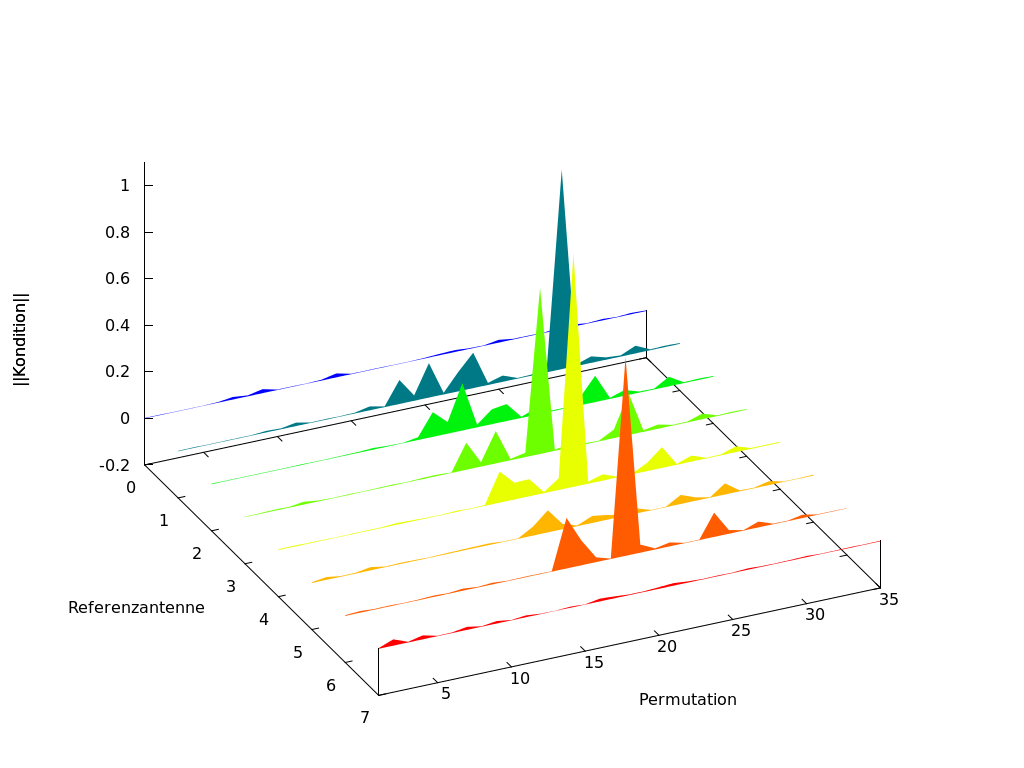
\includegraphics[width=\textwidth]{img/fenceModell3x3.png}
                 \caption{Konditionszahl der rein geometrischen $3\times3$ Matrix normiert auf den größten vorkommenden Wert ($=2149,16                 $)}
                 \label{fig:AnalyzeOf3x3}
         \end{subfigure}
%         
         \begin{subfigure}[h]{0.5\textwidth}
                 \centering
                 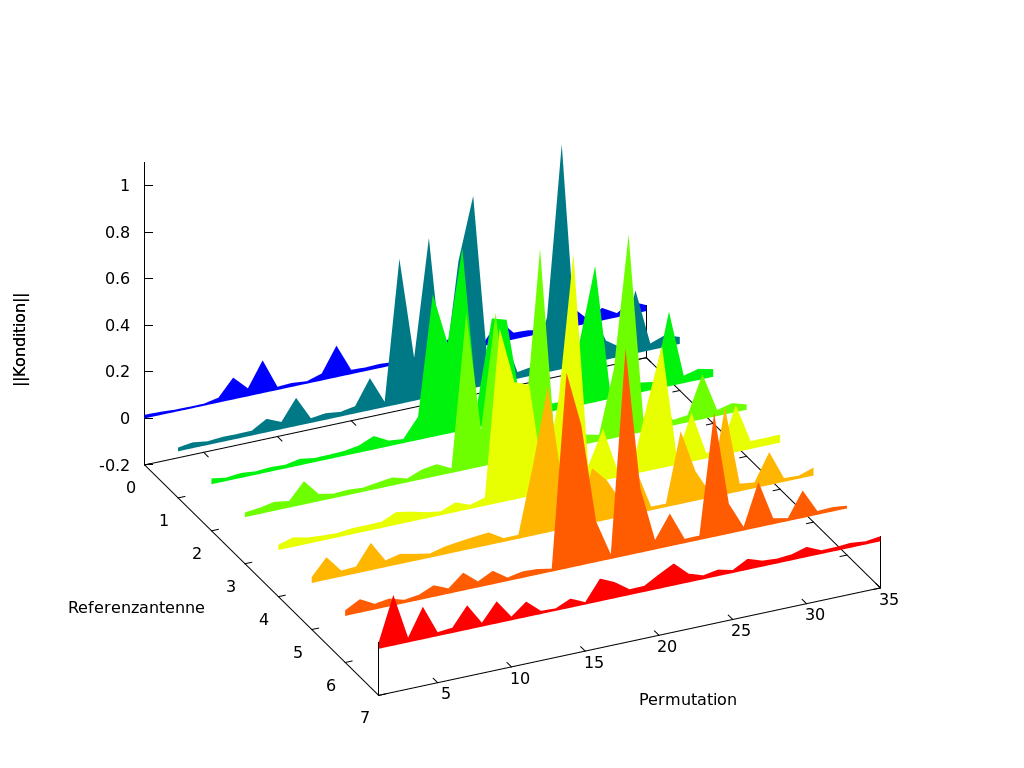
\includegraphics[width=\textwidth]{img/fenceModell9x3.png}
                 \caption{Konditionszahl der $10\times3$ Matrix normiert auf den größten vorkommenden Wert ($=257,13$); In dieser Konfiguration sind die Konstanten ($a_1$ \& $a_2$) sowie die variablen, gemessenen Phasen $\Theta_k$ enthalten}
                 \label{fig:AnalyzeOf10x3}
         \end{subfigure}
%
\end{figure}
%
Aus der Grafik lässt sich entnehmen, dass es für jede Referenzantenne aus der Geometrie alleine gute Konfigurationen existieren. Aus diesen Erkenntnissen kann in späteren Aufbauten, die Position der Antennen optimiert werden. Diese Verfahren wird in Abschnitt~\ref{sec:Calibration_Optimaztion} weiter beschrieben.
%
%- Section 2.3 --------------------------------------------------------------
\subsection{Weitere Anwendung der Konditionszahl}
Weitere Anwendungen, die sich aus der Konditionszahl der Matrix ableiten, sind denkbar. Für die FPGA-Software ist, parallel zu diesem Projekt, eine intelligente Umschaltung der Antennen in der Planung. Die Kondition der geometrische Matrix verändert sich nach dem Kalibrieren nicht mehr. Dadurch und durch die oben beschriebenen Überlegungen kann statisch eine Abschätzung für die Konditionszahl, von zwei der drei Blockmatrizen, im Vorfeld erstellt werden. Die Konditionszahl dient zum Steuern der Umschaltung. Ordner man die möglichen Konfiguration anhand ihrer Konditionszahl (niedrigste zuerst) in einer statischen Liste an so kann im FPGA eine einfache, schlaue Umschaltung implementiert werden. Diese würde immer dafür sorgen, dass Messdaten von einer Konfiguration bevorzugt werden, die eine niedrige Konditionszahl hat und somit relativ sicher zu einer guten Lösung führen. Diese überlegungen werden im Rahmen dieser Arbeit nicht näher beschrieben.\\
Eine Weitere Anwendung ergibt sich für die Kalibrierung. Der Aufbau der Antennen kann unter Berücksichtigung der Kondition optimieren. Ziel der Optimierung wäre es durch eine geeignete Positionierung der Antennen, die Anzahl der Antennenpermutationen mit kleiner Konditionszahl zu maximieren.
%
\section{Realisierung der Kalibrierung}
\label{sec:calibration}
In diesem Abschnitt wir die Implementierung der Kalibrierung des Messaufbaus und die Ergebnisse beschrieben. Es werden zwei unterschiedliche Berechnungsverfahren vorgestellt. Zuerst die Berechnung über das SVD-Verfahren, danach durch das CMA-ES-Verfahren. Es ist sinnvoll zu erwarten, dass beide Ergebnisse die gleichen Koordinaten liefern.
%
\subsection{Implementation}
%
Der Ablauf der Kalibrierung ist in Abbildung~\ref{fig:calibration_flowchart} in Form eine Ablaufdiagramms dargestellt. Beschrieben werden die wesentlichen Schritte. Es sind sowohl Interaktion mit der Person enthalten die die Kalibrierung durchführt, als auch die Schritte die von den beteiligten Softwarekomponenten ausgeführt werden enthalten. Es wurden im Rahmen der Arbeit zwei unterschiedliche Wege implementiert, ein Ergebnis für die Kalibrierung zu berechnen. Diese Wege werden nun kurz vorgestellt. Un die Ergebnisse mit einander verglichen. Die Präsentation der Resultate wird auch dazu verwendet werden die gewählte Form der Diagramme zu erläutern. Diese werden in den Ergebnissen des komplexeren Modells ebenfalls verwendet.
%
\begin{figure}[H]
	\begin{center}
		\caption[Ablauf der Kalibierung]{Ablauf der Kalibierung}
		\label{fig:calibration_flowchart}
		\vspace{0.5cm}
		\begin{tikzpicture}[auto]
		\scriptsize
			\tikzstyle{decision} = [diamond, draw=black, thick, fill=black!20, text width=5em, text badly centered, inner sep=1pt]
%			
			\tikzstyle{block} = [rectangle, draw=black, thick, fill=gray!20, text width=15em, text centered, rounded corners, minimum height=4em]
%	
			\tikzstyle{line} = [draw, thick, -latex',shorten >=1pt];
			\tikzstyle{commentline} = [draw, dashed, green!50,-latex',shorten >=1pt];
%	
			\tikzstyle{cloud} = [ dotted, draw=green!50, thick, ellipse,,fill=green!20, minimum height=2em, text width= 10em, text badly centered];
%	
			\matrix [column sep=5mm,row sep=7mm]
			{
				% row 1
				& \node [block] (start) { Start }; & \\
				% row 2
				& \node [block] (setup) {Aufstellen des Kalibrierstücks}; & 
					\node [cloud] (comment1) {Gezeigt in Abbildung \ref{fig:calib_piece}}; \\
				% row 4
				& \node [block] (measure) {Vermessen der Entfernungen zu den Antennen}; & 
					\node [cloud] (comment2) {z.B. mit Laser-Entfernungsmesser, gezeigt in Abbildung \ref{fig:laser_meter}}; \\
				% row 5
				&\node [block] (writefile) {Eintragen der Vermessenen Werte in Mashinenlesbare Datei}; &\\
				% row 6
				\node (temp){}; &\node [block] (startsw) {Starte die Kalibiersoftware}; &\\
				% row 7
				&\node [block] (viewresults) {Speichern der berechneten Werte}; &\\
				% row 8				
				& \node [decision] (decide) {$\Delta \geq \Delta_{max}$}; & 
					\node [cloud] (criteria) {Ergebnisse haben eine geringe Abweichung};\\
				% row 9
				& \node [block] (stop) {Ende}; & \\
			};
			
%
%			Draw the arrows
%
			\path (decide) -| node [near start] {Nein} (temp);
			\tikzstyle{every path}=[line]
			\path (start) -- (setup);
			\path (setup) -- (measure);
			\path (measure) -- (writefile);
			\path (writefile) -- (startsw);
			\path (startsw) -- (viewresults);
			\path (viewresults) -- (decide);
			\path (decide)	-| +(-3,0)  |- (measure);
			\path (decide) -- node [midway] {Ja} (stop);
			
%			
%			draw the comments 
%
			\tikzstyle{every path}=[commentline]
			\path (criteria) -- (decide);
			\path (comment1) -- (setup);
			\path (comment2) -- (measure);
				
		\end{tikzpicture}
	\end{center}
\end{figure}

\subsubsection{SVD}
%
Das unter \ref{sec:svd} vorgestellte Verfahren der Singular-Value-Decomposition kann dazu verwendet werden eine Lösung eines Gleichungssystems zu berechnen. Das Modell, dass zur Kalibrierung verwendet wird, ist ein Gleichungssystem der Form $\mathbf{b}=\mathbf{A}\mathbf{x}$ und hat drei Gleichungen mit drei Unbekannten. Daher kann sofort eine Lösung mit dem Verfahren hergeleitet werden. Das Ergebnis eines Messaufbaus mit 3 Antennen ist in Tabelle\ref{tab:FinalCoords} und in Abbildung~\ref{fig:3dplot_coordinates} gezeigt. Die Implementation des Algorithmus stammt aus \cite{press2007numerical} und wurde für diese Arbeit angeschafft.
%
\subsubsection{CMA-ES}
Das über den evolutionären Algorithmus gefundene Ergebnis gleicht dem des SVD-Verfahrens. Der SVD-Algorithmus ist um ein vielfaches effizienter beim Lösen des Gleichungssystems. Der Gründe warum an dieser Stelle das Ergebnis dennoch über evolutionäre Verfahren dargestellt wird sind folgende:
%
\begin{enumerate}
 \item Die Komplexität ist gering, daher kann der Ablauf des evolutionären Verfahrens besser dargestellt und verstanden werden
 \item Der Vergleich der beiden Ergebnisse ermöglicht die Verifizierung der Implementation beider Verfahren.
\end{enumerate}
%
Der erste Punkt kommt im Rahmen dieser Arbeit eine besondere Stellung zu, es ist einfacher anhand dieses Übersichtlichen Problems (mit nur drei Unbekannten) den Ablauf des Algorithmus sowie die Visualisierung der Ergebnisse besser zu erläutern. Die verwendete Darstellung gleicht der, die später bei dem Komplexeren Modell Verwendung findet.
%
\subsection{Ergebnis}
Es werden nun die Ergebnisse der Kalibrierung vorgestellt. Für eine der Vermessenen Antennenkonfigurationen sind in der folgenden Tabelle die Koordinaten der Antennen gezeigt. Die Visualisierung der Konfiguration zeigt die Abbildung~\ref{fig:3dplot_coordinates}.
%
\begin{table} [!ht]
	\begin{center}
		\begin{tabular}{cccc}
		      \textbf{Antenne} & \textbf{x} & \textbf{y} & \textbf{z} \\
		      1 &	0.479	&	-1.012 & 0.60 \\
		      2 &	-0.77 	&	-1.04 & 1.34 \\
		      3 &	1.52  	&	-1.05 & 1.37 \\
		      4 &	-0.92 	&	-0.19 & 1.32 \\
		      5 &	1.92 	&	0.03 & 1.39 \\
		      6 &	-0.55 	&	1.09 & 1.43 \\
		      7 &	1.06 	&	1.07 & 1.35 \\
		      8 &	0.45 	&	1.35 & 0.67 \\
%		      
		\end{tabular}
		\caption[Finale Antennen Koordinaten]{Tabelle der finalen Antennenkoordinaten [m], berechnet mit dem in dieser Arbeit entwickelten Modell und dem SVD-Verfahren, die Ergebnisse wurden auf zwei Nachkommastellen gerundet und sind identisch für beide Methoden.}
		\label{tab:FinalCoords}
	\end{center}
\end{table}
%
Eine Berechnung mit dem evolutionären Verfahren dauerte ca. $170~ms$ mit dem SVD-verfahren wurde eine Lösung und $\le 1~ms$ gefunden. Für die in der Praxis eingesetzte Software wird es eine Implementation der Kalibrierung mit dem SVD-Verfahren geben. Das Ergebnis der mit dieser Variante berechnete Verfahren wird bei Bedarf mit einer Lösung des evolutionären Verfahrens verglichen. Das ermöglicht eine Build-In Verifikation der Kalibrierung.\\

Für die in den folgenden Abbildungen präsentierten Ergebnisse wurden insgesamt $100$ Durchläufe des Algorithmus erstellt. Die Ergebnisse wurden mit einem vom Algorithmus selbst erstellten $\mu$ und $\lambda$ gefunden. In Abbildung~\ref{fig:Final_Calibration_Ant0_ES-boxes} wird eine statistische Auswertung der Ergebnisse gezeigt. In jedem Plot werden die Endwerte der Lösungen in einem sog. Boxplot gezeigt. Dabei wird die Verteilung mit Hilfe von Boxen dargestellt. Die Fähnchen der Boxen, stellen die maximal- bzw. minimal-Werte dar. Die Größe der Boxen enthält das obere und untere Quartil der Daten, der horizontale Strich in der Box zeigt den Mittelwert der Daten. Ausreißer in den Daten werden durch Punkte abseits der Box dargestellt.\\
%

Die Abbildung.~\ref{fig:Final_Calibration_Ant0_ES-boxes} zeigt den Verlauf der drei Objektvariablen (x,y,z-Koordinaten) sowie die Entwicklung der Fitness und des mittleren Sigmas. Als Darstellungsart wird der Linienplot verwendet und überlagern die Verläufe der einzelnen Lösungen. Das Abbruchkriterium war eine Fitness von $\leq 10^{-25}$. Für Darstellungszwecke wurde die x-Achse nach $500$ Werten beschränkt, erreicht der Fitness-Plot diesen Wert in der Abbildung nicht. Der Verlauf ist typisch für den Verwendeten Algorithmus. Deutlich zu erkennen ist eine Verbesserung des Ergebnisses mit steigender Zahl der Generationen. Der Verlauf der Variablen ist immer für den Erfolgreichsten Nachkommen einer Generation dargestellt.\\
%

Abbildung~\ref{fig:Final_Calibration_Ant0_ES-Scatter} ist ein Scatter-Plot. Die Objektvariablen werden hier gegeneinander aufgetragen. Auf der Diagonalen befinden sich stets die Variable mich sich selbst, daher zeigt sich dort eine Linie bzw. ein einzelner Punkt, sollten die Ergebnisse nicht streuen. Der Plot ist praktisch um die Implementation des Algorithmus zu verifizieren. Er lässt Rückschlüsse auf Abhängigkeiten und Einflüsse der Objektvariablen zu. So können die Ergebnisse mit den Erwartungen verglichen werden.\\
%
%---------------------------------------------------------------
%
\begin{figure}[!ht]
  \begin{center}
    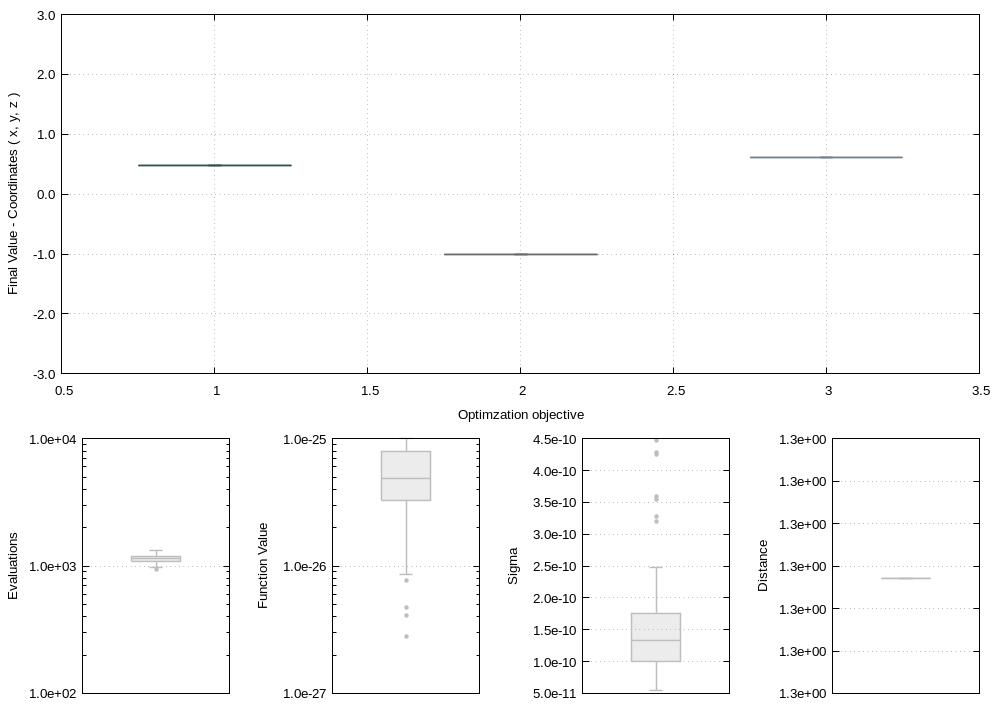
\includegraphics[width=0.9\textwidth]{img/calibration/calibration_ant0-boxes.png}
  \end{center}
  \caption {Boxplot des Kalibierergebnis aus $100$ Durchläufen. Im oberen Plot der sind die x,y,z-Koordinaten gezeigt, diese landen in allen Durchläufen auf dem selben Ergebnis. Das zeigt sich in der Breite der Linien. Die unteren vier Plots zeigen die Anzahl der Evaluationen der Fitness-Funktion, den finalen Funktionswert, das Sigma für die Variablen, die Entfernung zum Referenzpunkt (v.l.n.r.).}
  \label{fig:Final_Calibration_Ant0_ES-boxes}
%
\end{figure}
%
%---------------------------------------------------------------
%
\begin{figure}[!ht]
  \begin{center}
    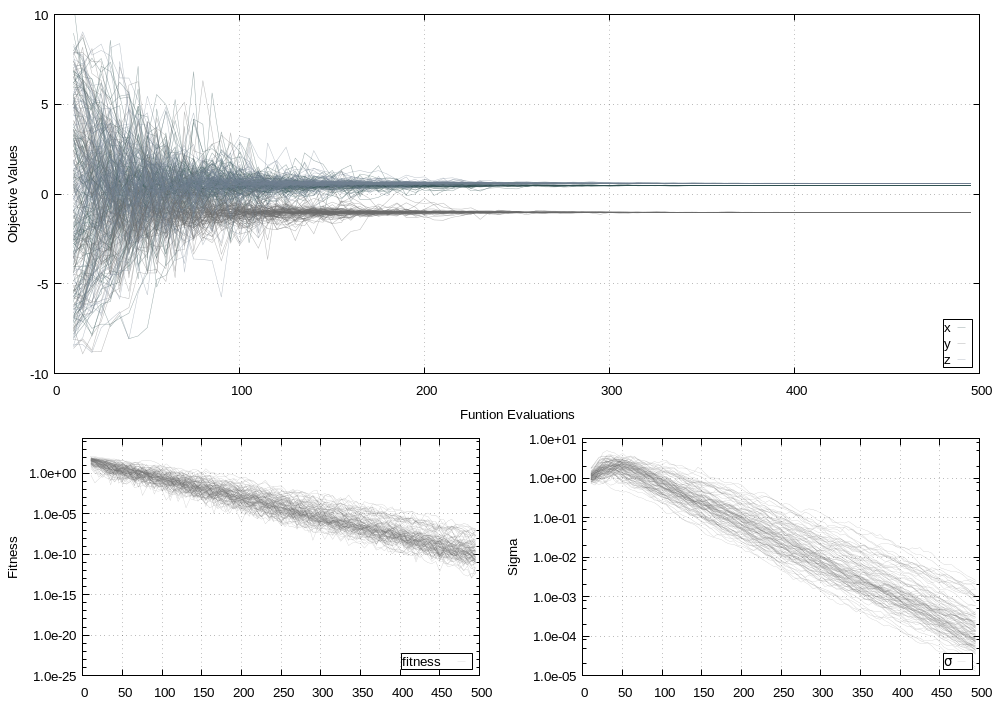
\includegraphics[width=0.9\textwidth]{img/calibration/calibration_ant0-lines.png}
  \end{center}
  \caption {Zu erkennen ist, das nach ca. 300 Evaluationen der Zielfunktion keine großen Änderungen der Variablen zu erkennen sind. Bis zum erreichen des Abbruchkriteriums (Function Value $\leq10^{-25}$) werden noch ca 400 Evaluationen benötigt, vgl. korrespondierender Boxplot.}
  \label{fig:Final_Calibration_Ant0_ES-Lines}  
%  
\end{figure}
%---------------------------------------------------------------
%
\begin{figure}[!ht]
  \begin{center}
    
\includegraphics[width=0.9\textwidth]{img/calibration/calibration_ant0-scatter.png}
  \end{center}
  \caption {Scatter-Plot der Ergebnisse der evolutionären Kalibrierung. Die Endergebnisse streuen in keiner Dimension, das wird aus dieser Darstellung deutlich.}
  \label{fig:Final_Calibration_Ant0_ES-Scatter}  
%  
\end{figure}
%---------------------------------------------------------------
%
\lipsum[1]
%
\begin{figure}[!ht]
         \centering
         \begin{subfigure}[h]{0.4\textwidth}
                 \centering
                 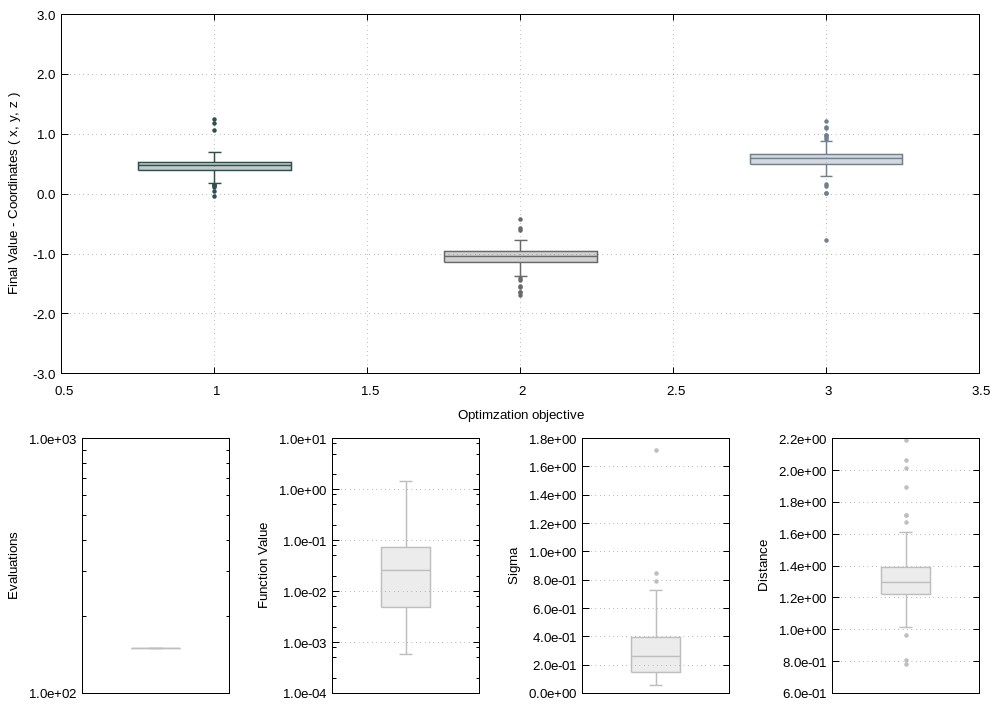
\includegraphics[width=\textwidth]{img/calibration/aborted_calibration_ant0-boxes.png}
                 \caption{Statistisch verteilte Endwerte für die Koordinaten der Kalibrierung. Die Werte für x,y, und z haben noch nicht ihren Endwert erreicht.}
                 \label{fig:abortedFinal_Calibration_Ant0_ES-boxes}
         \end{subfigure}
%
\qquad         
%
         \begin{subfigure}[h]{0.4\textwidth}
                 \centering
                 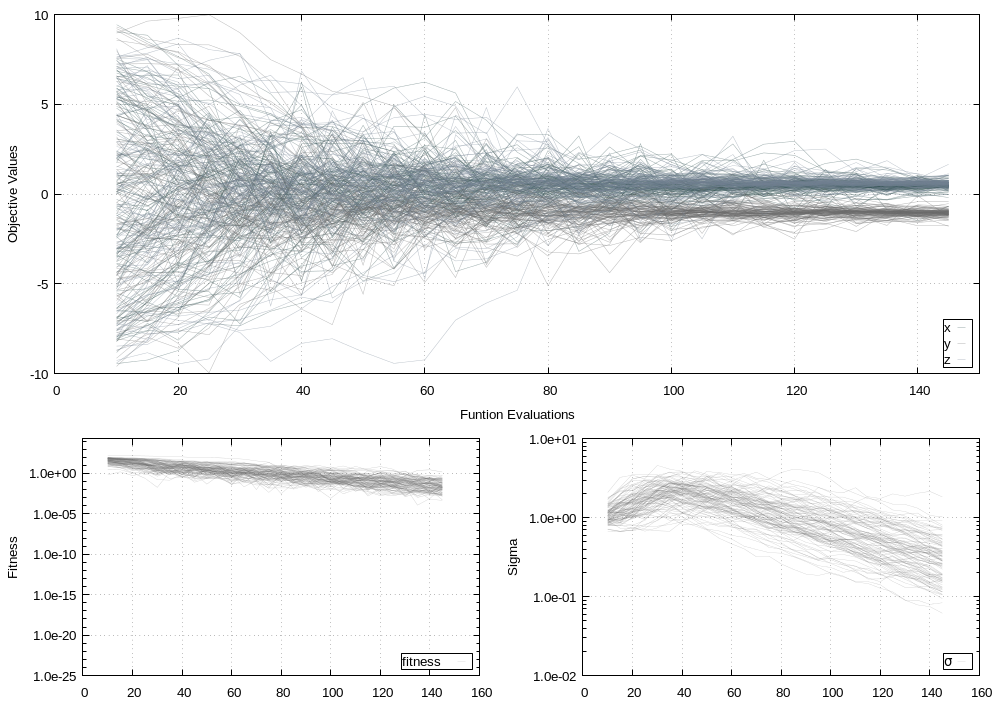
\includegraphics[width=\textwidth]{img/calibration/aborted_calibration_ant0-lines.png}
                 \caption{lorem}
                 \label{fig:abortedFinal_Calibration_Ant0_ES-Lines}
         \end{subfigure}
%
\\
%
         \begin{subfigure}[h]{0.4\textwidth}
                 \centering
                 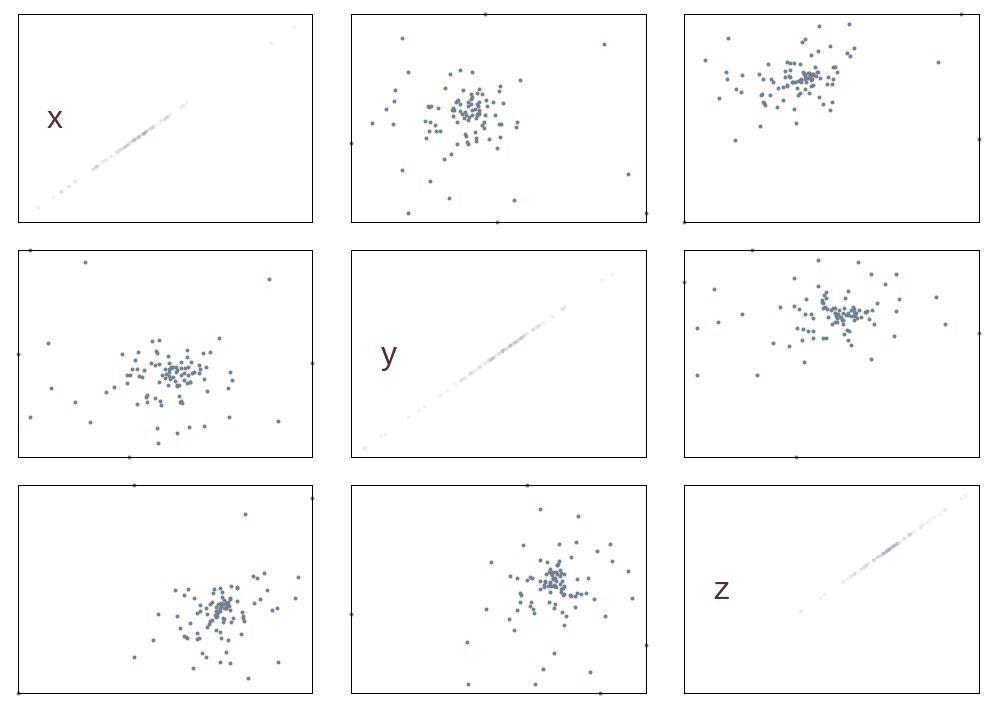
\includegraphics[width=\textwidth]{img/calibration/aborted_calibration_ant0-scatter.png}
                 \caption{lorem}
                 \label{fig:abortedFinal_Calibration_Ant0_ES-Scatter}
         \end{subfigure}
%
         \caption[Statistisch verteilte Ergebnisse der Evolutionären Kalibrierung]{Analog zu der Abbildung \ref{fig::Final_Calibration_Ant0} zeigen die Plots die gleichen Darstellungen. Diese zeigt, wie sich eine Statistische Verteilung in den Plots Manifestieren würde. Um das zu demonstrieren wurde das Abbruchkriterium auf lediglich $150$ Evaluationen der Zielfunktion eingestellt. Zu diesem Zeitpunkt können die Objektvariablen bereits einen passablen Wert erreicht haben oder noch abweichende Werte aufweisen (vgl. \ref{fig:Final_Calibration_Ant0_ES-Lines}).}
         \label{fig::abortedFinal_Calibration_Ant0_ES}
\end{figure}
%
\begin{figure}[ht!]
         \centering
         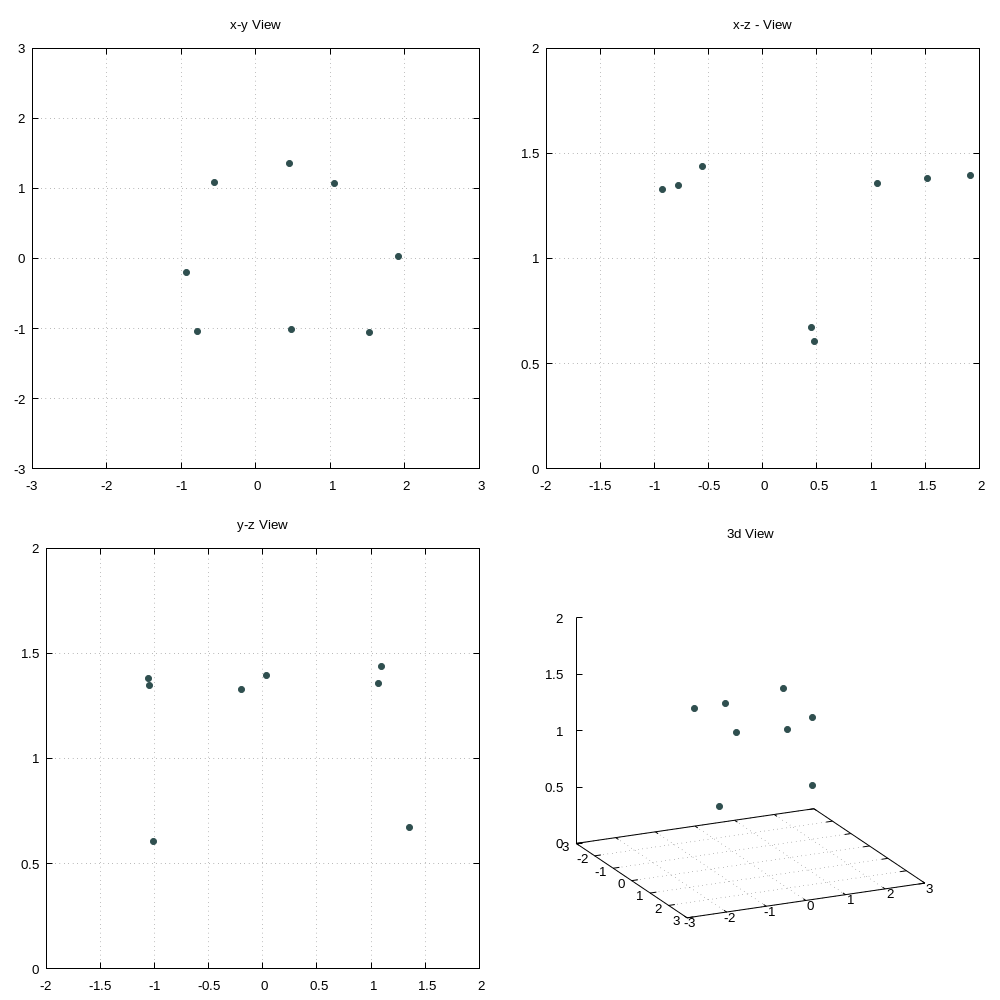
\includegraphics[width=0.7\textwidth]{img/calibration/calibration_results.png}
         \caption[Visualisierung des Kalibrierendergebnis]{Visualisierung des Kalibrierendergebnis. Abgebildet sind die gefundenen Antennenkoordinaten (Punkte) in drei Raumansichten. Die zusätzliche, dreidimensionale  Ansicht dient der Überischt.}
         \label{fig:3dplot_coordinates}
%
\end{figure}
%
\begin{figure}[ht!]
         \centering
         \caption[Kalibrierwerkzeuge]{Werkzeuge die bei der Kalibrierung verwendet werden.}
         \begin{subfigure}[h]{0.4\textwidth}
                 \centering
                 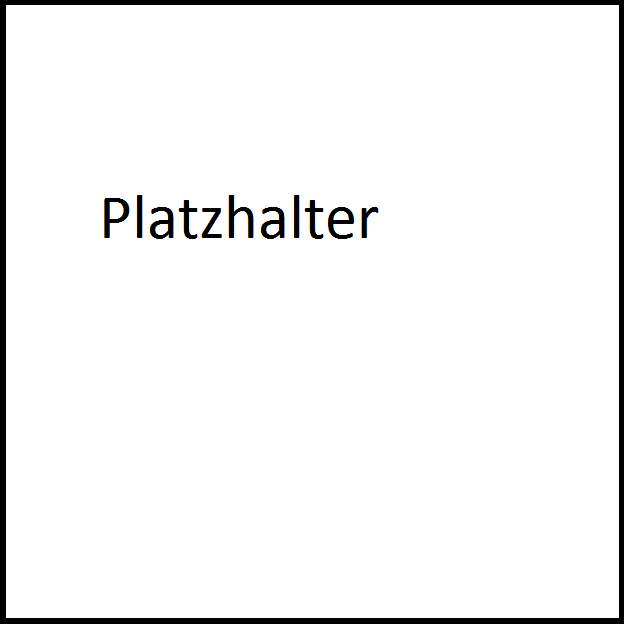
\includegraphics[width=\textwidth]{img/00_placeholder-sqare.png}
                 \caption{Laser Distanzmesser}
                 \label{fig:laser_meter}
         \end{subfigure}
%
\qquad         
%
         \begin{subfigure}[h]{0.4\textwidth}
                 \centering
                 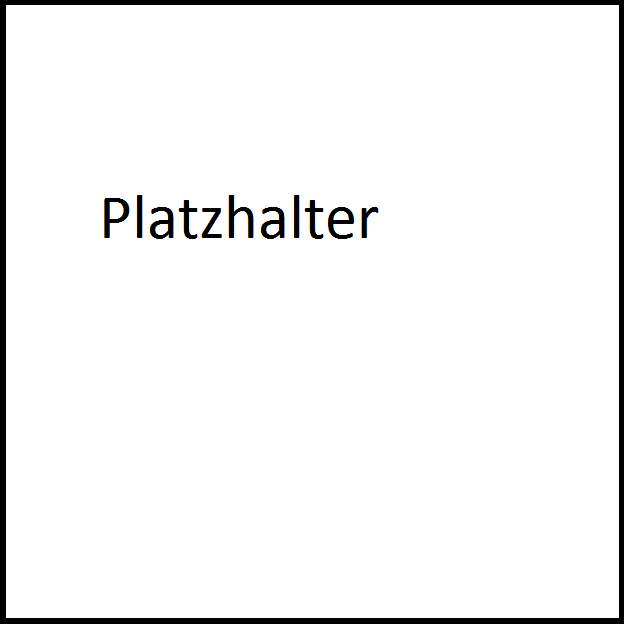
\includegraphics[width=\textwidth]{img/00_placeholder-sqare.png}
                 \caption{Kalibrierstück}
                 \label{fig:calib_piece}
         \end{subfigure}
         \label{fig:Calibration_Tools}
\end{figure}
 
%
%\subsection{Konkurierende Modelle}
% SuWi - Zeug 
%\lipsum[1-1]
%
\section{Betrachtung der Komplexität}
\label{sec:Komplexity2}
%
Im Folgenden wird eine Betrachtung der Komplexität des in Abschnitt~\ref{sec:model_developement} entwickelten Modells präsentiert. Diese Betrachtung ist wichtig für die Parametrisierung des Optimierungsverfahrens sowie für eine Beurteilung der Generellen Lösbarkeit mit den verwendeten Verfahren. Es wird eine Visualisierung des Fitness-Raums vorgestellt und im Vergleich mit sog. Benchmark-Funktionen diskutiert.\\
%

Für die Erstellung der Fitness-Ebenen wurde ein Programmteil (der \textit{FitnessPlaneCalculator}) entwickelt, der ein Modell mit vorgegebenen Daten füttert und den Rückgabewert in eine Datei schreibt. Das Programm lässt sich per Eingabedatei steuern und erlaubt die Definition der Ebenen die dargestellt werden sollen. Es lassen sich immer zwei Variablen der Objektfunktion variieren und der Rest wird dabei auf feste Werte gesetzt. Das erlaubt eine Visualisierung durch eine 2D-Heatmap (siehe folgende Plots). Aus der Visualisierung können Rückschlüsse auf die Gestalt der Fitnessebene gezogen werden.\\
%

Die Parameter wurde für diese Plots so gewählt das sie über einen Bereich iterieren, indem die richtige Lösung liegen sollten. Da nur drei Parameter variiert werden, werden die übrigen vier auf analytisch bestimmte, wahre Werte gesetzt. Diese sind in Tabelle~\ref{tab:complexity1} zusammen mit den wahren Werten aufgeführt.\\

%
\begin{figure}[h!]
  \caption[Fitness Ebenen Heatmap]{Diese Grafik zeigt die Fitnessebenen des Problems für eine Anordnung aus vier Antennen und einem Sweep über die $x-y$ - Ebene. Jeder Plot ist für einen festen Wert $z$ erstellt worden. In der Oberen linken Ecke beginnend und nach rechts laufend. Die $x, y$-Werte wurden über ein Intervall von $[-5,5]$ m und mit einem Inkrement von $0.2$ variiert. Daraus ergibt eine für die Abschätzung der Gestalt der Fitnessebene ausreichende Datengrundlage. Die $z$-Werte der $16$-Plots stammen aus dem Intervall $[-7,-7]$ mit einem Inkrement von $1$. Bereits in dieser Ansicht, ist zu erkennen, dass der Verlauf sehr Flach ist. Eine Schlucht bildet sich etwa in Nord-Süd-Richtung aus. Jeweils verzeichnet ist das lokale Minima ($+$) eins Plots, sowie die Höhenlinien\footnote{Die Höhenlinien sind für diskrete Werte ${0,1,10,40,50,100,200,500,1000}$ erstellt worden}. Die farbliche Kodierung gibt den Fitnesswert an diesem Punkt an. Die Fitnesswerte wurden normiert und um den Wert ihres Minimums verschoben.}
  \begin{center}
    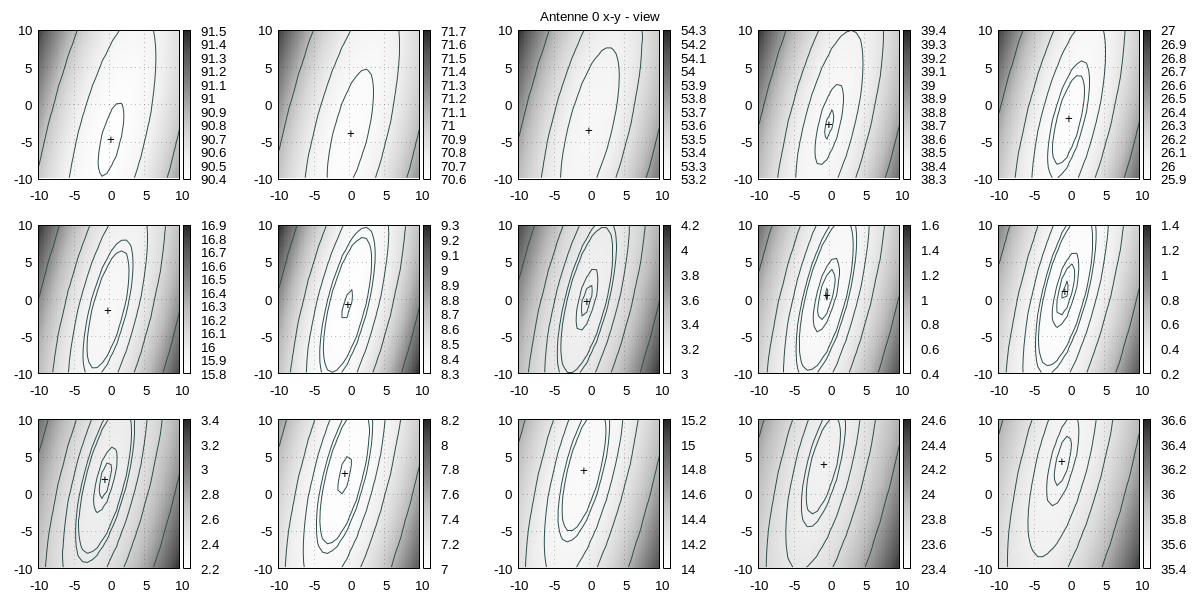
\includegraphics[width=\textwidth]{img/fitness/xy_a0.png}
  \end{center}
  \label{fig:fitnessplane1-x-y-1}
%
\end{figure}

\begin{figure}[ht!]
  \caption[Fitness Ebenen Heatmap, vergrößert]{Vergrößerung der Fitnessebenen der Antenne 1. Es ist hier deutlich zu erkennen, wie gering die Funktionen ansteigen. Das ist ein Problem für die meisten Algorithmen. Es bleibt zu klären wie sensitiv der Algorithmus auf diesen Umstand reagiert. Es wurde um das lokale Minima zentriert und der Bereich auf}
  \begin{center}
   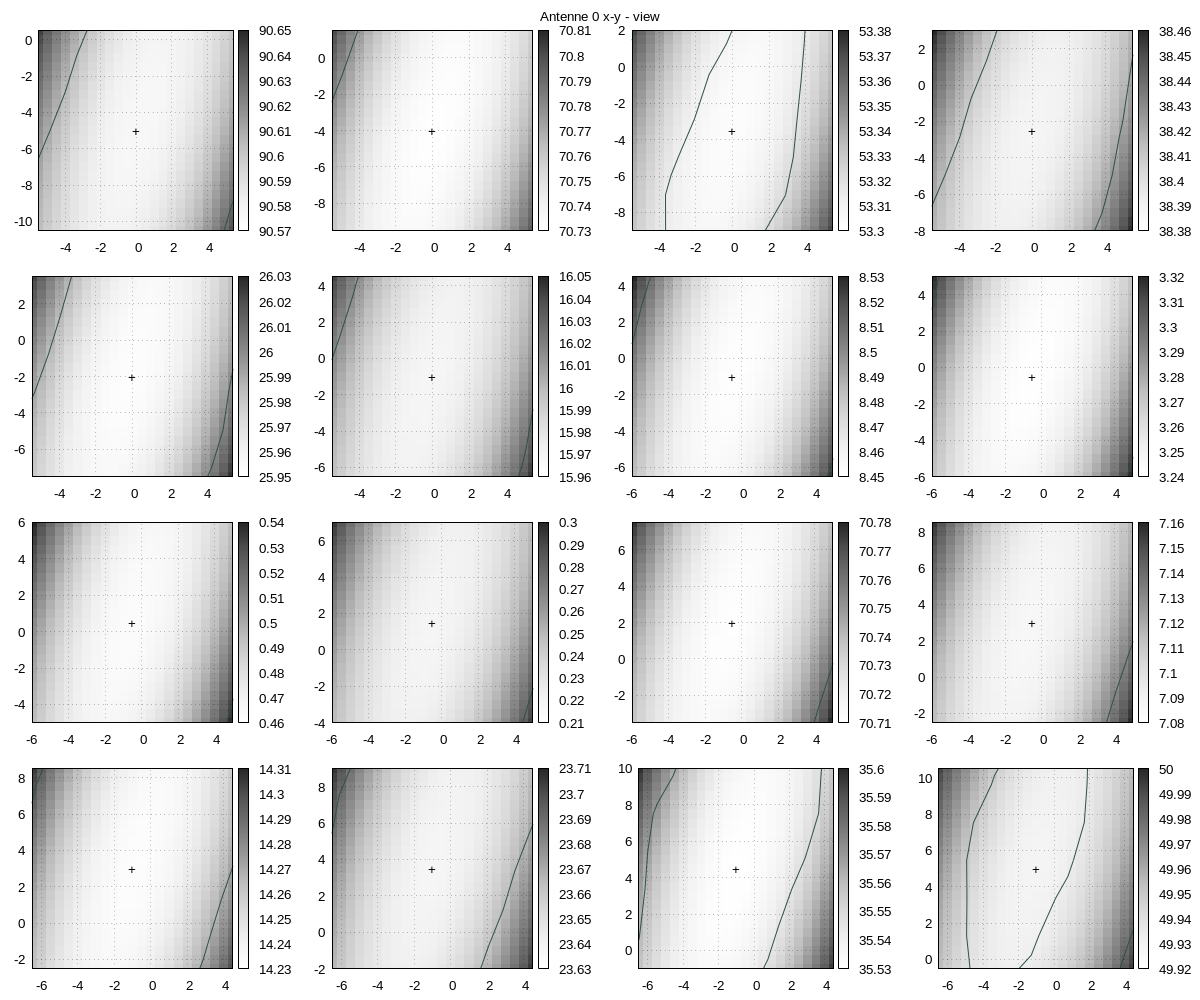
\includegraphics[width=\textwidth]{img/fitness/xy_a0zoomed.png}
  \end{center}
  \label{fig:fitnessplane1-x-y-zoom-1}
%
\end{figure}
%
In den Abbildungen~\ref{fig:fitnessplane1-x-y-1} und \ref{fig:fitnessplane1-x-y-zoom-1} zeigen sich möglicherweise die ersten Probleme für den Algorithmus. Eine große, sehr flache Fitnessebene für verschiedene Parameter ist nicht leicht zu handhaben. Aus dieser Untersuchung geht bereits hervor, dass die Anzahl an Nachkommen groß sein muss. Auch darf die Schrittweite $\sigma$ nicht zu klein werden, damit die Lösung nicht auf der flachen Ebene liegen bleibt. Ein Ähliches Verhalten zeigt sich bei den anderen Antennen und anderen Ebenen. Aufgrund der Komplexität des in dieser Arbeit erstellten Modells \ref{fig:Complexity1} ist bereits dieser Fall recht hochdimensional. Er erreicht $7$ Dimensionen und er kann im Rahmen dieser Arbeit nicht vollständig Untersucht werden. Die Fitness-Plots aller Antennen und für drei Ebenen sind in Anhang~\ref{app:fitness:plots1} zu finden. Eine vollständige Untersuchung ist indes auch nicht notwendig, da der Algorithmus den Suchraum in gewisser Weise untersucht. 
%
\begin{figure}[!h]
	 \caption[Übrige Ebenen für Antenne 1]{Auf diesen Abbildungen zeigen sich die Fitness-Ebenen für die übrigen Ansichten, x-z und y-z. In der oberen Reihe sind Ebenen über den gesamten Bereich, in der Unteren vergrößert dargestellt. Zu erkennen ist ein zum Verlauf der x-y-Ebene sehr ähnliches Bild. Ein flaches, längliches Tal mit Minimum.  }
	 \label{fig:fitnessplanesA1}
     \centering
     \begin{subfigure}[t]{0.4\textwidth}
             \centering
             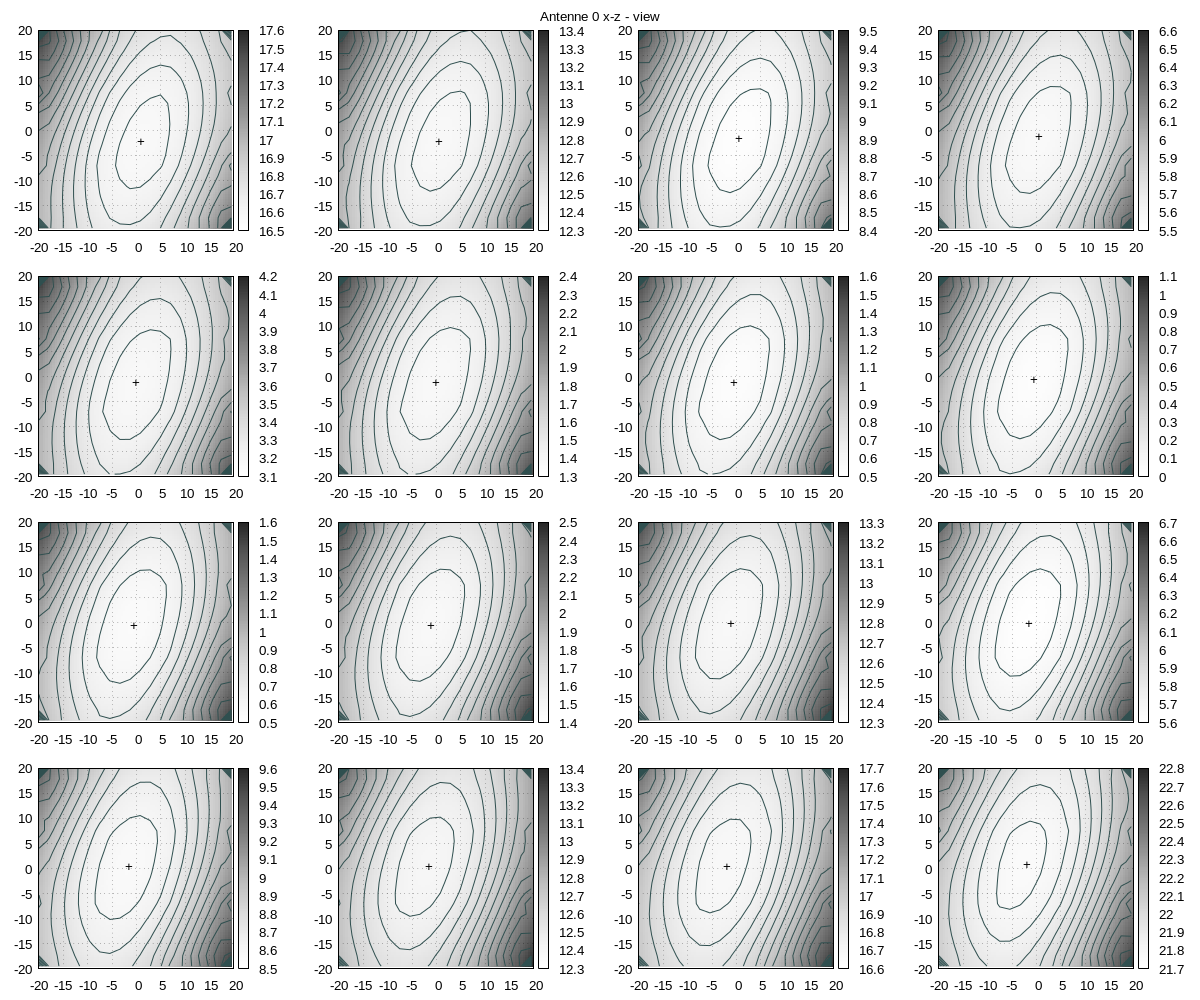
\includegraphics[width=\textwidth]{img/fitness/xz_a0.png}
%             \caption{Statistisch verteilte Endwerte für die Koordinaten der Kalibrierung.}
%             \label{fig:abortedFinal_Calibration_Ant0_ES-boxes}
     \end{subfigure}
     \qquad
     \begin{subfigure}[t]{0.4\textwidth}
			\centering
			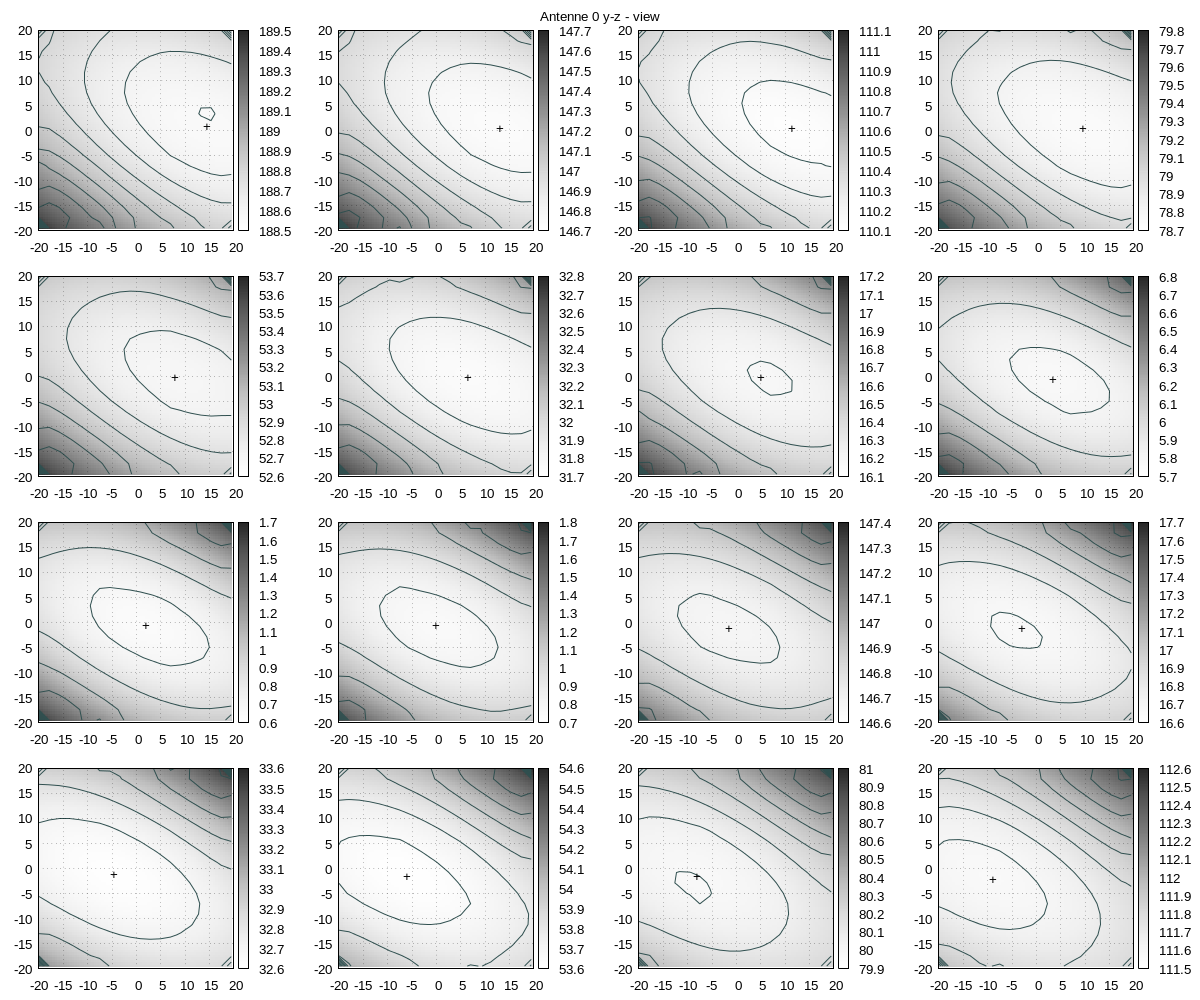
\includegraphics[width=\textwidth]{img/fitness/yz_a0.png}
%			\caption{x-z-Ebene, vergrößert}
%			\label{fig:abortedFinal_Calibration_Ant0_ES-boxes}
	 \end{subfigure}
\\
\vspace{5mm}
     \begin{subfigure}[t]{0.4\textwidth}
			\centering
			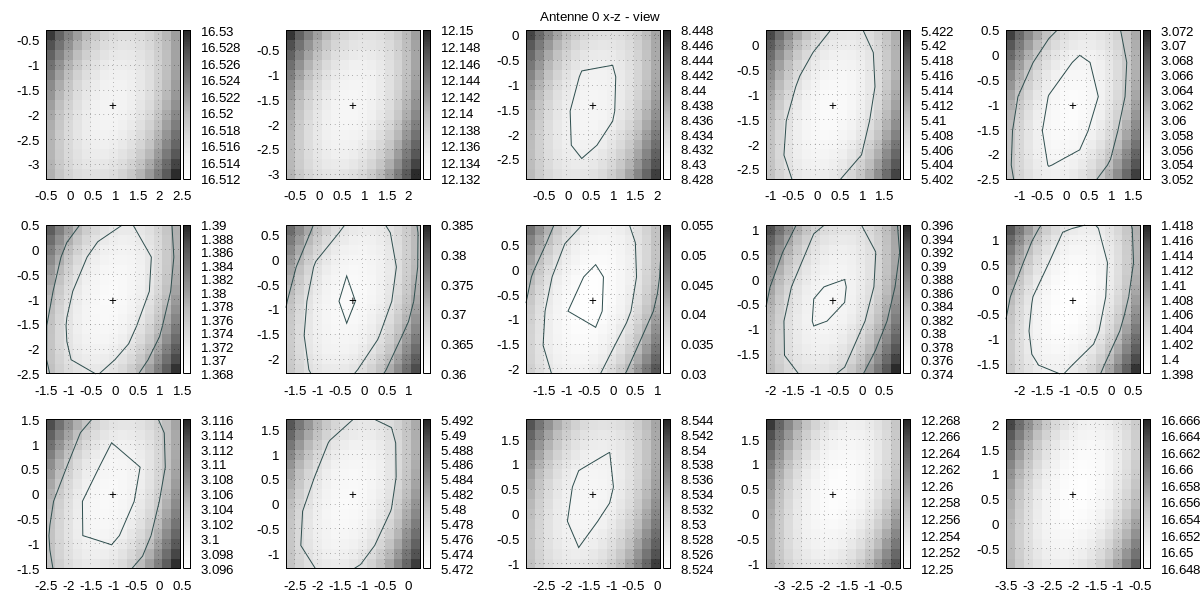
\includegraphics[width=\textwidth]{img/fitness/xz_a0zoomed.png}
%			\caption{x-z-Ebene, vergrößert}
%			\label{fig:abortedFinal_Calibration_Ant0_ES-boxes}
	 \end{subfigure}
	 \qquad
     \begin{subfigure}[t]{0.4\textwidth}
			\centering
			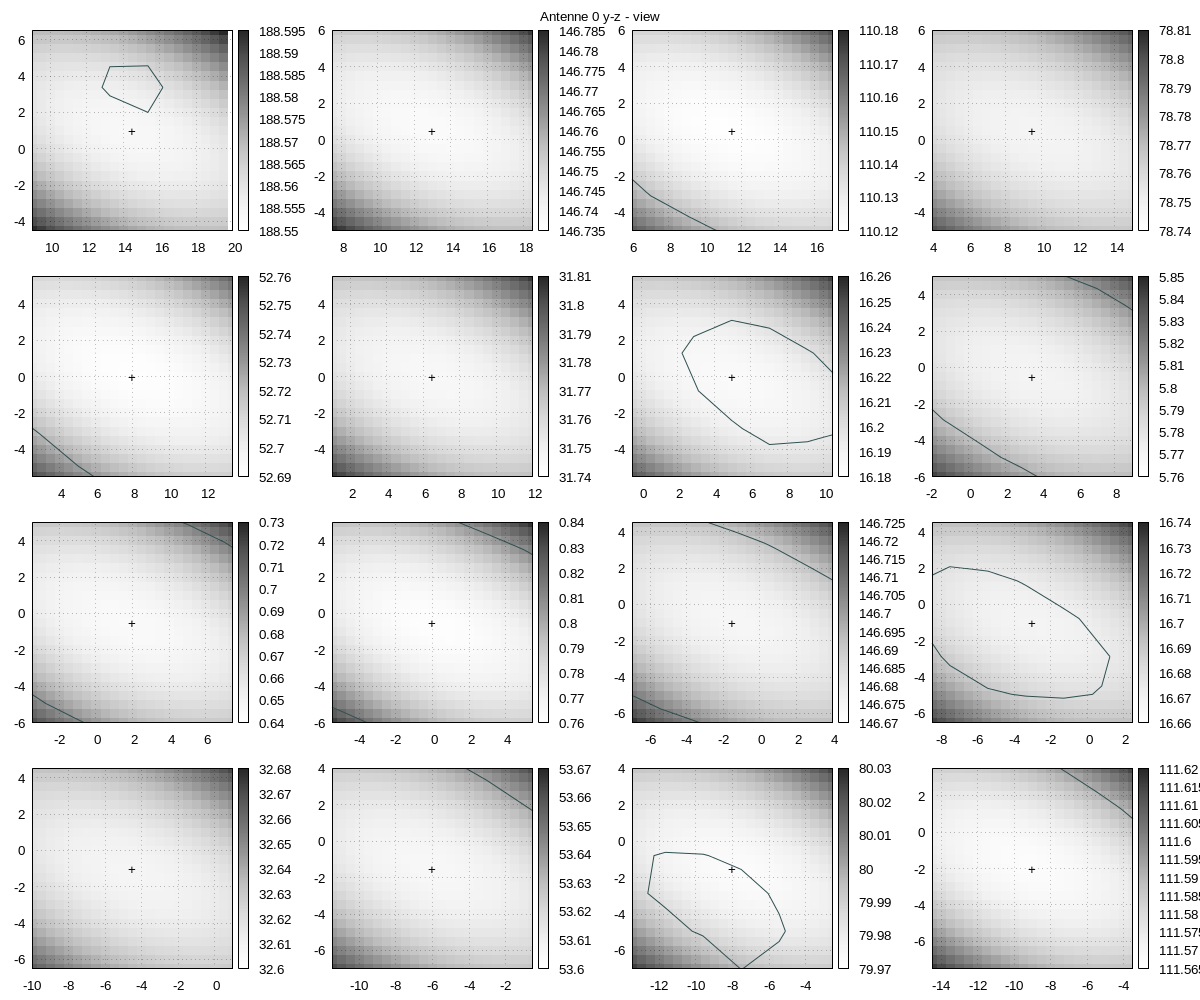
\includegraphics[width=\textwidth]{img/fitness/yz_a0zoomed.png}
%			\caption{x-z-Ebene, vergrößert}
%			\label{fig:abortedFinal_Calibration_Ant0_ES-boxes}
	 \end{subfigure}      
\end{figure}
%
\begin{table} [h]
	\begin{center}
		\begin{tabular}{lccccccc}
		\textbf{Ebene} & \textbf{$x$} & \textbf{$y$} & \textbf{$z$} & \textbf{$n_0$} & \textbf{$n_1$}& \textbf{$n_2$} & \textbf{$n_3$} \\
			\hline
			x-y & [-20:.5:20]		& [-20:.5:20]	& [-7:1:8] & [7:0:7] & [10:0:10]& [13:0:13]&[9:0:9]   \\
			x-z & [-20:.5:20] 	& [-7:1:8] 	& [-20:.5:20] & [7:0:7] & [10:0:10]& [13:0:13]&[9:0:9] \\
			y-z & [-7:1:8]  	& [-20:.5:20]	& [-20:.5:20] & [7:0:7] & [10:0:10]& [13:0:13]&[9:0:9]\\
			\hline
			Wahre & 0.479 & -1.012 & 0.607 & 7  & 10 & 13 & 9			\\
%
		\end{tabular}
		\caption[Parameter der Fitness Ebenen]{Tabellarisch sind hier die Parameter (Intervalle) der Fitness Ebenen aufgelistet. Zusätzlich sind die Werte angegeben, in denen eine optimale Lösung liegen sollte. }
		\label{tab:complexity1}
	\end{center}
\end{table}

\section{Software}
\label{sec:sw}
%
\lstset{
	basicstyle=\scriptsize,
	language=C++,
	breaklines=true,
	%		frameround=fttt,
	frame=tbrl,
	breakatwhitespace=false
	breaklines=true,  
	xleftmargin=1cm,
	tabsize=2,
	showstringspaces=false}
%---------------------------------------------------------------------
%
\subsection{Shark}
\label{sec:Shark}
Shark ist eine Open-Source \cpp Library für Maschinelles Lernen und Optimierung ~\cite{Shark:1}. Es Implementiert Methoden für lineare und nicht lineare Optimierung, Kernel-basierte Lernverfahren, künstliche neuronale Netzwerke, und Weitere. Details der Umsetzung finden sich in~\cite{shark08}. Es wird sowohl in Forschung als auch industriellem Umfeld eingesetzt und implementiert, nach eigenen Angaben, Algorithmen die in anderen Libraries nicht verfügbar sind. Shark baut auf den \textit{Boost C++ Libraries} auf und verwendet CMake\footnote{CMake (cross-platform make) ist ein plattformunabhängiges Programmierwerkzeug für die Entwicklung und Erstellung von Software.}. Dadurch ist es nahezu auf jeder Plattform verfügbar. Die Integration in ein Projekt ist sehr einfach und daher wird es in dieser Arbeit eingesetzt.\\

Eine Integration von Shark in dem Software Ökosystem ist aufgrund der vielen Features sehr sinnvoll. Weitere Entwicklungen können vom Funktionsumfang partizipieren.

%
%---------------------------------------------------------------------
\subsection{Implementation}
\label{sec:Implementation}
In diesem Abschnitt wird auf interessante Details der Softwareimplementation eingegangen. Es ist nicht möglich im vollen Umfang die Implementation der Softare besprechen, dafür ist die Software zu Umfangreich\footnote{Für diese Arbeit wurden ca. $5000$ Zeilen Quellcode erstellt - einzelne Modelle nicht mitgerechnet}. Lediglich sollen hier die Implementationen verschiedener Evolutionsalgorithmen unter Verwendung von Shark gezeigt werden. Verschiedene Algorithmen wurden in Kapitel~\ref{sec:es-common} Es wird beispielhaft die Implementation einer Objektfunktion beschrieben, wie sie typischerweise in Shark vorgenommen wird.
%
%\begin{figure}[ht!]
	\begin{center}
		\caption[Integration PRPS Software]{Übersicht über die Integration des PRPS Evolution Moduls in die bestehende PRPS-Software}
		\label{fig:Integration-prpsevolutions}
		\vspace{1cm}
		\begin{tikzpicture}[auto]
		\scriptsize
			\tikzstyle{decision} = [diamond, draw=black, thick, fill=black!20, text width=5em, text badly centered, inner sep=1pt]
%			
			\tikzstyle{block} = [rectangle, draw=black, thick, fill=gray!20, text width=15em, text centered, rounded corners, minimum height=4em]
%	
			\tikzstyle{line} = [draw, thick, -latex',shorten >=1pt];
			\tikzstyle{commentline} = [draw, dashed, green!50,-latex',shorten >=1pt];
%	
			\tikzstyle{cloud} = [ dotted, draw=green!50, thick, ellipse,,fill=green!20, minimum height=2em, text width= 10em, text badly centered];
%	
			\matrix [column sep=5mm,row sep=7mm]
			{
				% row 1
				& \node [block] (start) { Start }; & \\
				% row 2
				& \node [block] (setup) {Aufstellen des Kalibrierstücks}; & 
					\node [cloud] (comment1) {Gezeigt in Abbildung \ref{fig:calib_piece}}; \\
				% row 4
				& \node [block] (measure) {Vermessen der Entfernungen zu den Antennen}; & 
					\node [cloud] (comment2) {z.B. mit Laser-Entfernungsmesser, gezeigt in Abbildung \ref{fig:laser_meter}}; \\
				% row 5
				&\node [block] (writefile) {Eintragen der Vermessenen Werte in Maschinenlesbare Datei}; &\\
				% row 6
				\node (temp){}; &\node [block] (startsw) {Starte die Kalibiersoftware}; &\\
				% row 7
				&\node [block] (viewresults) {Speichern der berechneten Werte}; &\\
				% row 8				
				& \node [decision] (decide) {$\Delta \geq \Delta_{max}$}; & 
					\node [cloud] (criteria) {Ergebnisse haben eine geringe Abweichung};\\
				% row 9
				& \node [block] (stop) {Ende}; & \\
			};
			
%
%			Draw the arrows
%
			\path (decide) -| node [near start] {Nein} (temp);
%			\tikzstyle{every path}=[line]
%			\path (start) -- (setup);
%			\path (setup) -- (measure);
%			\path (measure) -- (writefile);
%			\path (writefile) -- (startsw);
%			\path (startsw) -- (viewresults);
%			\path (viewresults) -- (decide);
%			\path (decide)	-| +(-3,0)  |- (measure);
%			\path (decide) -- node [midway] {Ja} (stop);
			
%			
%			draw the comments 
%
			\tikzstyle{every path}=[commentline]
%			\path (criteria) -- (decide);
%			\path (comment1) -- (setup);
%			\path (comment2) -- (measure);
				
		\end{tikzpicture}
	\end{center}
\end{figure}
%\newpage
%
%---------------------------------------------------------------------
\subsubsection{Objektfunktion in Shark}
\label{sec:Shark_model}
%
Als Beispiel für die Implementation einer Objektfunktion wird im Folgenden das Modell der evolutionären Kalibrierung besprochen. Dieses Modell, bzw. Objektfunktion, hat eine überschaubare Komplexität und wurde bereits im Abschnitt~\ref{sec:calibration} zur Veranschaulichung verwendet. Daher eignet es sich gut um die Implementation zu zeigen. Im Rahmen dieser Arbeit sind eine Vielzahl von Modellen entstanden, die nicht in aller Ausführlichkeit diskutiert werden können.\\
%
%---------------------------------------------------------------------
Das Listing~\ref{lst:EvolutionaryCalibration.h} zeigt die Headerdatei für die Implementation einer Objektfunktion, sofort ist zu erkennen, das sie von der abstakten Klasse \textit{SingleObjectiveFunction} abgeleitet ist. Diese ist einer von Shark bereitgestellte Klasse. Sie beschreibt die Funktionen die eine Objektfunktion implementieren muss damit sie von Optimizern verwendet werden kann. Ein von dieser Klasse abgeleitetes Modell erlaubt die Verwendung in verschiedenen Algorithmen. Die Funktion:
%
\begin{lstlisting}
double eval(const SearchPointType &p) const;
\end{lstlisting}
%
wird in von den Optimizern aufgerufen und implementiert die eigentliche Funktion des Modells.
%
\begin{lstlisting}[label=EvolutionaryCalibration_2]
void proposeStartingPoint(SearchPointType &x) const;
\end{lstlisting}
%
Diese Methode wird von einem Solver beim Start aufgerufen und liefert passende Startwerte für das Modell zurück. Der Rückgabewert der Funktion ist ein gleichverteilter Vektor der Dimension \textit{m\_numberOfVariables} in einem Intervall von $[-10,10]$ zurück. Der Wert für \textit{m\_numberOfVariables} wird bei der Instanziierung des Modells, beim Aufruf des Konstruktors, gesetzt. Dort wird auch die Eigenschaft \textit{CAN\_PROPOSE\_STARTING\_POINT} gesetzt, sie wird von den unterschiedlichen Optimizern verwendet um zu erkennen, welche Features vom Modell unterstützt werden.
%
\begin{lstlisting}[label=EvolutionaryCalibration_3]
	EvolutionaryCalibration( ) {
	m_numberOfVariables = Solve::ProblemDimensions::Calibration;
	m_features |= CAN_PROPOSE_STARTING_POINT;
}
\end{lstlisting}	
%
%---------------------------------------------------------------------
%
\lstinputlisting[caption=Quellcode Schnipsel für die Deklaration einer Objektfunktion \vspace{2mm},
				firstline=18, lastline=108, label=lst:EvolutionaryCalibration.h]{src/EvolutionaryCalibration.h}
%
Die in Listig~\ref{lst:EvolutionaryCalibration.cpp} gezeigte cpp-Datei ist die Implementation der oben beschriebenen Modellfunktionen. Aus diesen beiden Dateien ist ersichtlich, dass die Deklaration des Modells sehr überschaubar ist. Praktische jedes Modell hat diese übersichtliche Struktur, das erhöht die Wartbarkeit enorm. Außerdem erlaubt es einen einfachen Austausch in der Implementation sowie die Verwendung in unterschiedlichen Algorithmen. 
%
\begin{lstlisting}[label=EvolutionaryCalibration_4]
inline double EvolutionaryCalibration::mkII( const NRmatrix<Doub> &A, const double* x, const NRvector<Doub> &b ) const
\end{lstlisting}
%
Diese Funktion ist die eigentliche Berechnung des Gleichungssystems der Form $\mathbf{A}\mathbf{x}=\textbf{b}$. Die Lösung wird an die Aufrufende Funktion übergeben. Als Eingabe wird der Variablenvektor \textit{const double*x} von Shark sowie die geom. Matrix $\mathbf{A}$ und der Distanzvektor $\mathbf{b}$ erwartet.
%
Der vollständige Quellcode des Modells ist im Anhang~\ref{app:EvolutionaryCalibration1} und \ref{app:EvolutionaryCalibration2} gelistet.
%
%---------------------------------------------------------------------
%
\lstinputlisting[caption=Quellcode Schnipsel für die Implementation einer Objektfunktion für verschiedene Optimzier im Shark\vspace{2mm},
				 firstline=7, lastline=44, label=lst:EvolutionaryCalibration.cpp]{src/EvolutionaryCalibration.cpp}
%
%
\subsection{Process MkII - Finde die Lösung}

%
\subsection{Paralleler Ablauf}
\label{parallel_computing}
%
Die \textit{ProcessMkII}-Klasse ist Threadfähig. Eine Implementierung wurde im Rahmen der Arbeit durchgeführt. Durch das parallele Ablaufen verschiedener Optimierungen kann die Performance wesentlicher verbessert werden und so die Multi-Kern-Architektur aktueller Rechner ausgenutzt werden. Einen großen Beitrag zur schnellen Umsetzung lieferte der neue Standard \cpp11. Dieser Implementiert ein High-Level Konstrukt für Threads und Tasks, sodass es einfacher ist, Abläufe zu Synchronisieren und Ergebnisse abzufragen. Zusätzlich ist die Implementation sehr leicht, wie im folgenden Listing gezeigt:
%
\lstinputlisting[caption=Erstellen von mehreren Threads bei gleichzeitiger Übergabe der Parameter\vspace{2mm},
				 firstline=1, lastline=19]{src/async.cpp}
				 \label{lst:Parallel_example1.cpp}
%
\vspace{2mm}
Das Abfragen der Ergebnisse ist genauso einfach:
\vspace{2mm}
%
\lstinputlisting[caption=Abfragen der Asynchronen Ergebnisse mit Hilfe des auto-Datentyp. Ausgabe des Ergebnisses in einer Datei.\vspace{2mm},
				 firstline=23, lastline=36]{src/async.cpp}
				 \label{lst:Parallel_example2.cpp}
%
\vspace{2mm}
%
\subsection{Schnittstelle für Dateneingabe}
%
Im Folgenden wird die implementierte Schnittstelle besprochen mit der die Daten unter den Programmteilen ausgetauscht werden können. Die Schnittstelle umfasst im Wesentliche zwei Teile:
\begin{enumerate}
	\item Eingabe für die gemessenen Phasenwerte
	\item Ausgabe für die ermittelten Wellenzahlen
\end{enumerate}
%
Hinzukommt eine pseudo-Schnittstelle über die die Systemparameter eingelesen werden können. Die aktuelle Implementation ließt lediglich eine CSV-Eingabedatei, mit den Systemparametern in eine entsprechende Struktur ein. Diese Parameter stehen Anschließend dem PRPS-Evolution System zur Verfügung.
%
Die Kommunikation zwischen dem PRPS-Dienst und dem PRPS-Evolution ist einfach. Der Dienst teilt die gemessenen Phasendaten mit, die vom PRPS-Evolution für die Berechnung der Wellenzahlen verwendet werden. Das bedeutet das der Ablauf des Auffindens der Wellenzahl vom PRPS-Dienst als 'Black-Box' angesehen wird.\\
%
%\subsubsection{Schnittstelle für Dateneingabe}
%
\subsection{Ablaufdiagramme}
%
Vieles der Funktionalität der Software ist zu umfangreich für dieses Dokument. Es kann in diesem Rahmen keine vollständige Besprechung des Quellcodes durchgeführt werden. Wichtige Funktionalitäten und Abläufe werden in Ablaufplänen zusammenfassend dargestellt.
%
\begin{figure}[h]
	\begin{center}
		\caption[Ablauf Programmstart]{Prozessschritte nach Start des Programms}
		\label{fig:start_programm}
		\vspace{0.5cm}
		\begin{tikzpicture}[auto]
		\scriptsize
			\tikzstyle{decision} = [diamond, draw=black, thick, fill=black!20, text width=5em, text badly centered, inner sep=1pt]
%			
			\tikzstyle{block} = [rectangle, draw=black, thick, fill=gray!20, text width=15em, text centered, rounded corners, minimum height=4em]
%	
			\tikzstyle{line} = [draw, thick, -latex',shorten >=1pt];
			\tikzstyle{commentline} = [draw, dashed, green!50,-latex',shorten >=1pt];
%	
			\tikzstyle{cloud} = [ dotted, draw=green!50, thick, ellipse,,fill=green!20, minimum height=2em, text width= 10em, text badly centered];
%	
			\matrix [column sep=5mm,row sep=7mm]
			{
				% row 1
				& \node [block] (start) { Start }; & \\
				% row 2
				&\node [block] (load) {Lade System}; &  \\
				% row 3
				&\node [block] (perm) {Generiere Permutationen}; & \\
				% row 4
				& \node [block] (preprocess) {Vorberechnung der Matrizen}; & \\
				% row 5
				& \node [block] (stop) {Ende}; & \\
			};
% Arrows
			\tikzstyle{every path}=[line]
			\path (start) -- (load);
			\path (load) -- (perm);
			\path (perm) -- (preprocess);
			\path (preprocess) -- (stop);
%		
%			\tikzstyle{every path}=[commentline]
%			\path (criteria) -- (decide);
%			\path (comment1) -- (init);
%			
			
		\end{tikzpicture}
	\end{center}
\end{figure}
%
\begin{figure}[h]
	\begin{center}
		\caption[Finde Modelllösung]{Schritte die zur Lösungsfindung abgearbeitet werden. Dies ist ein Teil des Hauptprogramms, der die erstellten Informationen vom Programmstart in ein Modell zum Auffinden einer Lösung übergibt. Es werden eine beliebige Anzahl an Lösungen generiert.}
		\label{fig:find_model_solution}
		\vspace{0.5cm}
		\begin{tikzpicture}[auto]
		\scriptsize
			\tikzstyle{decision} = [diamond, draw=black, thick, fill=black!20, text width=5em, text badly centered, inner sep=1pt]
%			
			\tikzstyle{block} = [rectangle, draw=black, thick, fill=gray!20, text width=15em, text centered, rounded corners, minimum height=4em]
%	
			\tikzstyle{line} = [draw, thick, -latex',shorten >=1pt];
			\tikzstyle{commentline} = [draw, dashed, green!50,-latex',shorten >=1pt];
%	
			\tikzstyle{cloud} = [ dotted, draw=green!40, thick, ellipse,,fill=green!10, minimum height=2em, text width= 12em, text badly centered];
%	
			\matrix [column sep=5mm,row sep=7mm]
			{
				% row 1
				& \node [block] (start) { Start }; & \\
				% row 2
				&\node [block] (load) {Lade Phasendaten vom Interface}; &  
					\node [cloud] (comment3) {Verschiedene Quellen sind mögliche (z.B. CSV-Datei, Stream etc.) }; \\
				% row 3
				&\node [block] (create1) {Erstelle '\textit{preprocess}'-Instanz}; & 
					\node [cloud] (comment4) {Berechne die möglichen Matrizen; Treffe Auswahl an 'guten' Matizen für die Lösung }; \\
				%
				&\node [block] (create) {Erstelle '\textit{process}'-Instanz}; & 
					\node [cloud] (comment5) {Übergebe benötigte Informationen) }; \\
				% row 4
				& \node [block] (call) {Lösung für Modell finden:\\ process.\textit{model}()}; & 
					\node [cloud] (comment1) {Finde Lösung für '\textit{model}' - mehrere Modelle sind in '\textit{process}' implementiert}; \\
				% row 5
				& \node [decision] (decide) {$i==N$}; & 
					\node [cloud] (comment2) {Anzahl der Lösungen $N$ erreicht?}; \\
				% row 6
				& \node [block] (write) { Rufe '\textit{post-processing}' auf }; & \\
				% row 7
				& \node [block] (stop) {Ende}; & \\
			};
% Arrows
			\tikzstyle{every path}=[line]
			\path (start) -- (load);
			\path (load) -- (create1);
			\path (create1) -- (create);
			\path (create) -- (call);
			\path (call) -- (decide);
%		
			\path (decide) -- node [near start] {[Ja]} (write);
			\path (decide) -|  node [above] {[Nein] - i++;} +(-2,0) -- node [] {} +(-3.5,0) |-  (call);
			
			\path (write) -- (stop);
%			
			\tikzstyle{every path}=[commentline]
			
			\path (comment1) -- (call);
			\path (comment2) -- (decide);
			\path (comment3) -- (load);
			\path (comment4) -- (create1);
			\path (comment5) -- (create);
%			
		\end{tikzpicture}
	\end{center}
\end{figure}
%
\begin{figure}[h]
	\begin{center}
		\caption[Modelllösung bestimmen]{Die Grafik zeigt den Ablauf im Modell um eine Lösung zu finden. Es werden so lange Evolutionsschritte durchgeführt bis das Konvergenzkriterium erreicht wird.}
		\label{fig:find_model_solution}
		\vspace{0.5cm}
		\begin{tikzpicture}[auto]
		\scriptsize
			\tikzstyle{decision} = [diamond, draw=black, thick, fill=black!20, text width=5em, text badly centered, inner sep=1pt]
%			
			\tikzstyle{block} = [rectangle, draw=black, thick, fill=gray!20, text width=15em, text centered, rounded corners, minimum height=4em]
%	
			\tikzstyle{line} = [draw, thick, -latex',shorten >=1pt];
			\tikzstyle{commentline} = [draw, dashed, gray!50,-latex',shorten >=1pt];
%	
			\tikzstyle{cloud} = [ dotted, draw=gray!50, thick, ellipse,,fill=gray!5, minimum height=2em, text width= 10em, text badly centered];
%			\tikzstyle{cloud} = [ dotted, draw=green!40, thick, ellipse,,fill=green!10, minimum height=1em, text width= 15em, text badly centered];
%	
			\matrix [column sep=5mm,row sep=7mm]
			{
%			 row 1
				& \node [block] (start) { Start }; & \\
%	 row 2
				&\node [block] (create1) {Erstelle '\textit{model}'-Instanz}; & \\
%	 row 3
				&\node [block] (set1) {Setze Anzahl der Objektvariablen}; & 
					\node [cloud] (comment1) { Teile dem Modell die Anzahl der Veränderlichen mit, der Solver verwendet später diese Initialisierung }; \\
				
				&\node [block] (set2) {Set Modell-Parameter}; & 
					\node [cloud] (comment2) { Die Modelle erhalten unterschiedliche Parameter, z.B. die ausgewählten Matrizen }; \\
%	 row 4
				& \node [block] (create2) {Erstelle Instanz von \textit{CMA-ES-Solver}}; & 
					\node [cloud] (comment3) {Hier wird das Modell aufgerufen }; \\
				& \node [block] (init) {Parametrisiere den Solver}; & 
					\node [cloud] (comment4) { Einstellen von $\lambda$ und $\mu$ sowie Lösungsstrategie}; \\
%	 row 5
				& \node [block] (step) {cma.\textit{step}()}; & \\
				
				& \node [decision] (decide) {Optimum reached?}; & 
					\node [cloud] (comment5) {Konvergenzkriterium erreicht? (z.B. Ziel-Fitness, max. Evaluationen erreicht etc.)}; \\
%	 row 6
				& \node [block] (done) {done\\ \textbf{return final-solution}}; & \\
			};
% Arrows
			\tikzstyle{every path}=[line]
			\path (start) -- (create1);
			\path (create1) -- (set1);
			\path (set1) -- (set2);
			\path (set2) -- (create2);
			\path (create2) -- (init);
			\path (init) -- (step);
			\path (step) -- (decide);
%		
			\path (decide) -- node [near start] {[Ja]} (done);
			\path (decide) -|  node [above] {[Nein] - i++;} +(-2,0) -- node [] {} +(-3.5,0) |-  (step);
		
%			
			\tikzstyle{every path}=[commentline]
			
			\path (comment1) -- (set1);
			\path (comment2) -- (set2);
			\path (comment3) -- (create2);
			\path (comment4) -- (init);
			\path (comment5) -- (decide);
%			
		\end{tikzpicture}
	\end{center}
\end{figure}
%\begin{figure}[h]
%	\begin{center}
%		\caption[Modellablauf mit CMA-ES]{Ablauf im Modell; Der hier dargestellte Ablauf ist exemplarisch für alle in dieser Arbeit entstandenen Modelle; Die Modelle Variieren nur minimal }
%		\label{fig:struct_model}
%		\vspace{0.5cm}
%		\begin{tikzpicture}[auto]
%		\scriptsize
%			\tikzstyle{decision} = [diamond, draw=black, thick, fill=black!20, text width=5em, text badly centered, inner sep=1pt]
%%			
%			\tikzstyle{block} = [rectangle, draw=black, thick, fill=gray!20, text width=15em, text centered, rounded corners, minimum height=4em]
%%	
%			\tikzstyle{line} = [draw, thick, -latex',shorten >=1pt];
%			\tikzstyle{commentline} = [draw, dashed, green!50,-latex',shorten >=1pt];
%%	
%			\tikzstyle{cloud} = [ dotted, draw=green!40, thick, ellipse,,fill=green!10, minimum height=2em, text width= 12em, text badly centered];
%%	
%			\matrix [column sep=5mm,row sep=7mm]
%			{
%				% row 1
%%				& \node [block] (start) { Start }; & \\
%				% row 2
%%				&\node [block] (create1) {Erstelle '\textit{model}'-Instanz}; & \\
%				% row 3
%%				&\node [block] (set1) {Setze Anzahl der Objektvariablen}; & 
%%					\node [cloud] (comment2) { Teile dem Modell die Anzahl der Veränderlichen mit, der Solver verwendet später diese Initialisierung }; \\
%				%
%%				&\node [block] (set2) {Set Modell-Parameter}; & 
%%					\node [cloud] (comment2) { Die Modelle erhalten unterschiedliche Parameter, z.B. die ausgewählten Matrizen }; \\
%				% row 4
%%				& \node [block] (create2) {Erstelle Instanz von \textit{CMA-ES-Solver}}; & 
%%					\node [cloud] (comment1) {Hier wird das Modell aufgerufen }; \\
%%				& \node [block] (init) {Parametrisiere den Solver}; & 
%%					\node [cloud] (comment3) { Auswahl von $\lambda$ und $\mu$ sowie Lösungsstrategie}; \\
%				% row 5
%%				& \node [block] (step) {cma.\textit{step}()}; & \\
%				%
%%				& \node [decision] (decide) {Optimum reached?}; & 
%%					\node [cloud] (comment4) {Konvergenzkriterium erreicht? (z.B. Ziel-Fitness, max. Evaluationen erreicht etc.)}; \\
%				% row 6
%%				& \node [block] (done) {done}; & \\
%
%			};
%			
%% Arrows
%%			\tikzstyle{every path}=[line]
%%			\path (start) -- (create1);
%%			\path (create1) -- (set1);
%%			\path (set1) -- (set2);
%%			\path (set2) -- (create2);
%%			\path (create2) -- (init);
%%			\path (init) -- (step);
%%			\path (step) -- (decide);
%%%		
%%			\path (decide) -- node [near start] {[Ja]} (done);
%%			\path (decide) -|  node [above] {[Nein] - i++;} +(-2,0) -- node [] {} +(-3.5,0) |-  (call);
%%			
%%			\path (write) -- (stop);
%%%			
%%			\tikzstyle{every path}=[commentline]
%%			
%%			\path (comment1) -- (call);
%%			\path (comment2) -- (decide);
%%			\path (comment3) -- (load);
%%			\path (comment4) -- (create1);
%%			\path (comment5) -- (create);
%%			
%		\end{tikzpicture}
%	\end{center}
%\end{figure}
%

%\lipsum[1-5]
\lipsum[1-3]

%\section{Hardware}
%\label{sec:hw}
%\lipsum[1-3]


%
% 3. ------------------------------------------------------------------------
\chapter{Ergebnisse und Erkenntnisse}
In diesem Kapitel werden die Ergebnisse der Arbeit präsentiert. Zuerst werden künstliche Werte für die gemessene Phase als Eingabe für den Algorithmus verwendet. Darauf folgend werden reale Messdaten als Input verwendet und die Resultate verglichen. Abschließend werden weitere Erkenntnisse präsentiert, die während der Arbeit gewonnen werden konnten.\\
%
%\section{Ergebnisse}
%
\subsection{Ergebnis}
Es werden nun die Ergebnisse der Kalibrierung vorgestellt. Für eine der vermessenen Antennenkonfigurationen sind in der folgenden Tabelle die Koordinaten der Antennen gezeigt. Die Visualisierung der Konfiguration zeigt die Abbildung~\ref{fig:3dplot_coordinates}.
%
\begin{table} [ht!]
	\begin{center}
		\begin{tabular}{cccccccc}
		      \textbf{Antenne} & \textbf{$x$} & \textbf{$y$} & \textbf{$z$} & \textbf{$d_{meas}$} & \textbf{$d_{result}$}& \textbf{$\varepsilon_{abs}$} & \textbf{$\varepsilon_{rel}$} \\
		      1 & 0.48		& -1.01	& 0.60 & 1,259 & 1,274& 0,015 & 1,14\% \\
		      2 & -0.77 	& -1.04 	& 1.34 & 1,894 & 1,872 & -0,022 & 1,19\% \\
		      3 & 1.52  	& -1.05 	& 1.37 & 2,334 & 2,307 & -0,027 & 1,15\% \\
		      4 & -0.92 	& -0.19 	& 1.32 & 1,661 & 1,628 & -0,033 & 2,01\% \\
		      5 & 1.92 		&  0.03 	& 1.39 & 2,399 & 2,375 & -0,024 & 1,01\% \\
		      6 & -0.55 	&  1.09 	& 1.43 & 1,851 & 1,887 & 0,036 & 1,93\% \\
		      7 & 1.06 		&  1.07 	& 1.35 & 2,055 & 2,031 & -0,024 & 1,19\% \\
		      8 & 0.45 		&  1.35 	& 0.67 & 1,574 & 1,578 & 0,004 & 0,26\% \\					
%
		\end{tabular}
		\caption[Finale Antennen Koordinaten]{Tabelle der finalen Antennenkoordinaten [m], berechnet mit dem in dieser Arbeit entwickelten Modell und dem SVD-Verfahren. Die Ergebnisse wurden auf zwei Nachkommastellen gerundet und sind identisch für beide Methoden. Die Spalte $d_{result}$ enthält die von der Berechnung gefundenen Distanz vom Referenzpunkt zur Antenne. Die Spalte $d_{meas}$ zeigt die gemessenen Werte. Die $\epsilon$-Spalten zeigen die Abweichung.}
		\label{tab:FinalCoords}
	\end{center}
\end{table}
%
Eine Berechnung mit dem evolutionären Verfahren dauerte ca. $170$~ms mit dem SVD-verfahren wurde eine Lösung in $\le 1$~ms gefunden. Für die in der Praxis eingesetzte Software wird es eine Implementation der Kalibrierung mit dem SVD-Verfahren geben. Das mit dieser Variante berechnete Ergebnis wird bei Bedarf mit einer Lösung des evolutionären Verfahrens verglichen. Das ermöglicht eine Build-In Verifikation der Kalibrierung.\\

\subsubsection{Visualisierung der Ergebnisse}
Für die in den folgenden Abbildungen präsentierten Ergebnisse wurden insgesamt $100$ Durchläufe des Algorithmus erstellt. Die Ergebnisse wurden mit einem vom Algorithmus selbst erstellten $\mu$ und $\lambda$ gefunden. In Abbildung~\ref{fig:Final_Calibration_Ant0_ES-boxes} wird eine statistische Auswertung der Ergebnisse gezeigt. In jedem Plot werden die Endwerte der Lösungen in einem sog. Boxplot gezeigt. Dabei wird die Verteilung mit Hilfe von Boxen dargestellt. Die Fähnchen der Boxen stellen die maximal- bzw. minimal-Werte dar. Die Größe der Boxen enthält das obere und untere Quartil der Daten, der horizontale Strich in der Box zeigt den Mittelwert der Daten. Ausreißer\footnote{Hier Werte die mindestens den $2$-Fachen Wert des oberen- bzw. unteren-Quartils aufweisen} in den Daten werden durch Punkte abseits der Box dargestellt.\\
%

Die Abbildung~\ref{fig:Final_Calibration_Ant0_ES-boxes} zeigt den Verlauf der drei Objektvariablen ($x,y,z$-Koordinaten) sowie die Entwicklung der Fitness und des mittleren Sigmas. Als Darstellungsart wird der Linienplot verwendet und die Verläufe einzelner Lösungen überlagern sich in diesem Plot. Das Abbruchkriterium war eine Fitness von $\leq 10^{-25}$.% Ist Fitness nicht etwas gutes und sollte maximiert werden?
Für Darstellungszwecke wurde die $x$-Achse nach $500$ Werten beschränkt, daher erreicht der Fitness-Plot diesen Wert in der Abbildung nicht. Der Verlauf ist typisch für den verwendeten Algorithmus. Deutlich zu erkennen ist eine Verbesserung des Ergebnisses mit steigender Zahl der Generationen. Der Verlauf der Variablen ist immer für den erfolgreichsten Nachkommen einer Generation dargestellt.\\
%

Abbildung~\ref{fig:Final_Calibration_Ant0_ES-Scatter} ist ein Scatter-Plot. Die Objektvariablen werden hier gegeneinander aufgetragen. Auf der Diagonalen befinden sich stets die Variable gegen sich selbst aufgetragen, daher zeigt sich dort immer eine Linie, bei streuenden Ergebnissen, bzw. ein einzelner Punkt, sollten die Ergebnisse nicht streuen. Der Plot ist praktisch um die Implementation des Algorithmus zu verifizieren. Er lässt Rückschlüsse auf Abhängigkeiten und Einflüsse der Objektvariablen zu. So können die Ergebnisse mit den Erwartungen an die Verläufe verglichen werden.\\
%
%---------------------------------------------------------------
%
\begin{figure}[!ht]
  \begin{center}
   \caption[Box-Plot der Endergebnisse der Kalibierung]{Boxplot des Kalibierergebnis aus $100$ Durchläufen. Im oberen Plot sind die x,y,z-Koordinaten gezeigt, diese landen in allen Durchläufen auf dem selben Ergebnis. Was nicht verwundert, das Problem ist eines der Art \glqq{}drei Gleichungen und drei Unbekannte\grqq. Die Streuung der Lösung zeigt sich in der Breite der Linien. Die unteren vier Plots zeigen die Anzahl der Evaluationen der Fitness-Funktion, den finalen Funktionswert, das Sigma für die Variablen und die Entfernung zum Referenzpunkt (v.l.n.r.). Das Ergebnis sind die Koordinaten für Antenne 1}
    \label{fig:Final_Calibration_Ant0_ES-boxes}
    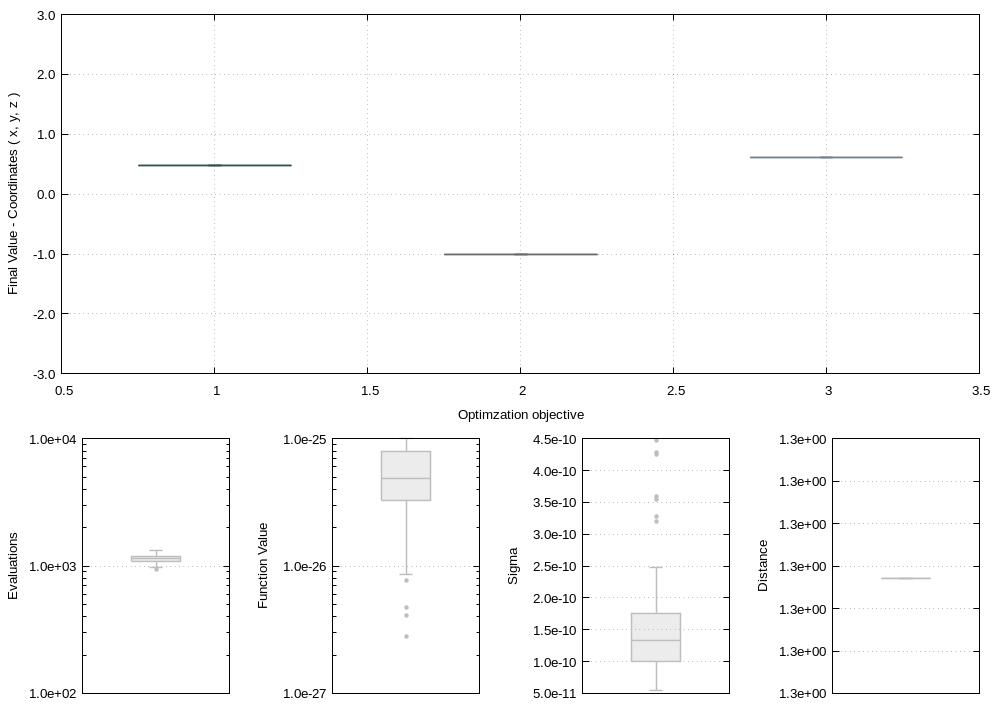
\includegraphics[width=0.9\textwidth]{img/calibration/calibration_ant0-boxes.png}
  \end{center}
 
%
\end{figure}
%
%---------------------------------------------------------------
%
\begin{figure}[!ht]
  \begin{center}
    \caption[Linien-Plot der Endergebnisse der Kalibierung]{Zu erkennen ist, dass nach ca. 300 Evaluationen der Zielfunktion keine großen Änderungen der Variablen zu erkennen sind. Bis zum erreichen des Abbruchkriteriums (Function Value $\leq10^{-25}$) werden noch ca 400 Evaluationen benötigt, vgl. korrespondierender Boxplot.}
    \label{fig:Final_Calibration_Ant0_ES-Lines}  
    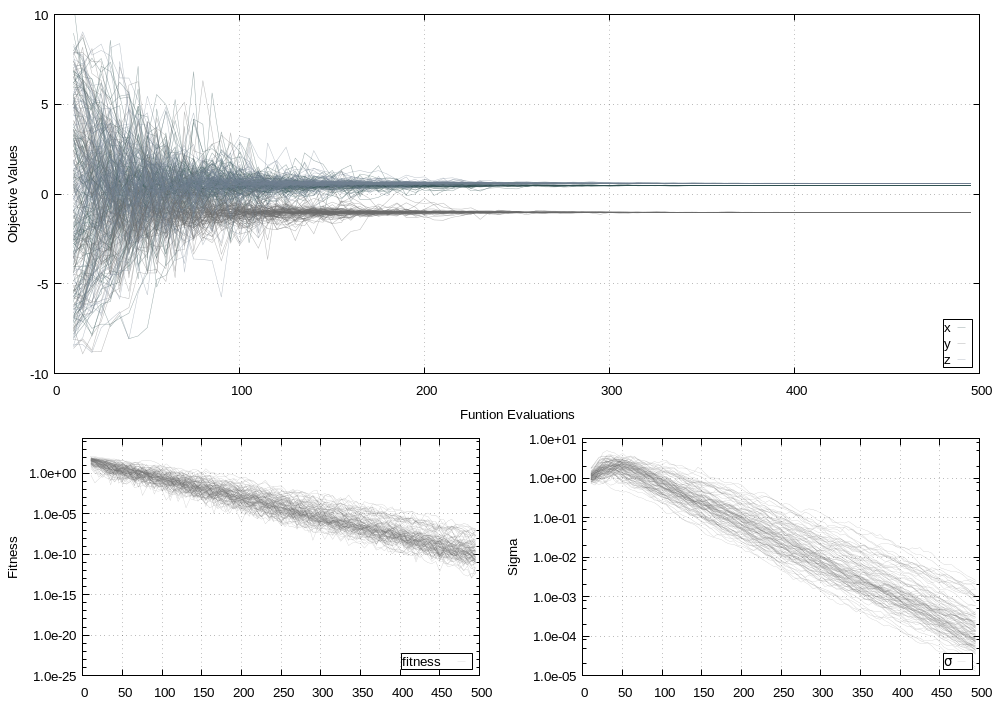
\includegraphics[width=0.9\textwidth]{img/calibration/calibration_ant0-lines.png}
  \end{center}
%  
\end{figure}
%---------------------------------------------------------------
%
\begin{figure}[!ht]
  \begin{center}
  
    \caption[Kalibierung Scatter-Plot]{Scatter-Plot der Ergebnisse der evolutionären Kalibrierung. Die Endergebnisse streuen in keiner Dimension, das wird aus dieser Darstellung deutlich.}
    \label{fig:Final_Calibration_Ant0_ES-Scatter}  
    
\includegraphics[width=0.9\textwidth]{img/calibration/calibration_ant0-scatter.png}
  \end{center}
%  
\end{figure}
%---------------------------------------------------------------
%
\begin{figure}[!ht]
     \centering
     \begin{subfigure}[t]{0.45\textwidth}
             \centering
             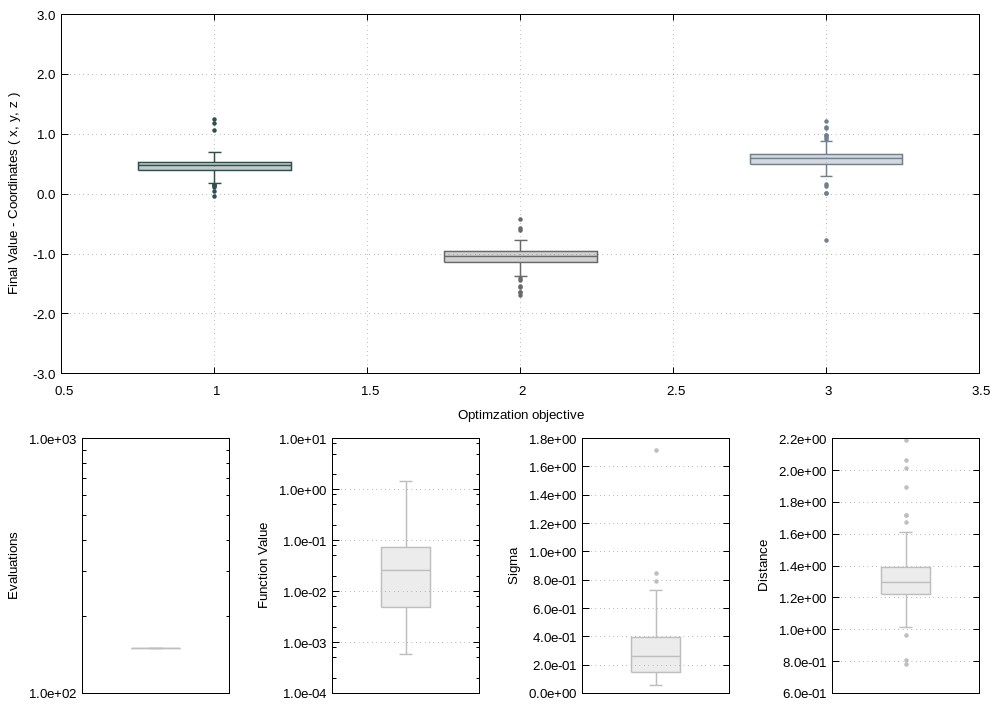
\includegraphics[width=\textwidth]{img/calibration/aborted_calibration_ant0-boxes.png}
             \caption{Statistisch verteilte Endwerte für die Koordinaten der Kalibrierung.}
             \label{fig:abortedFinal_Calibration_Ant0_ES-boxes}
     \end{subfigure}
%
\qquad         
%
     \begin{subfigure}[t]{0.45\textwidth}
             \centering
             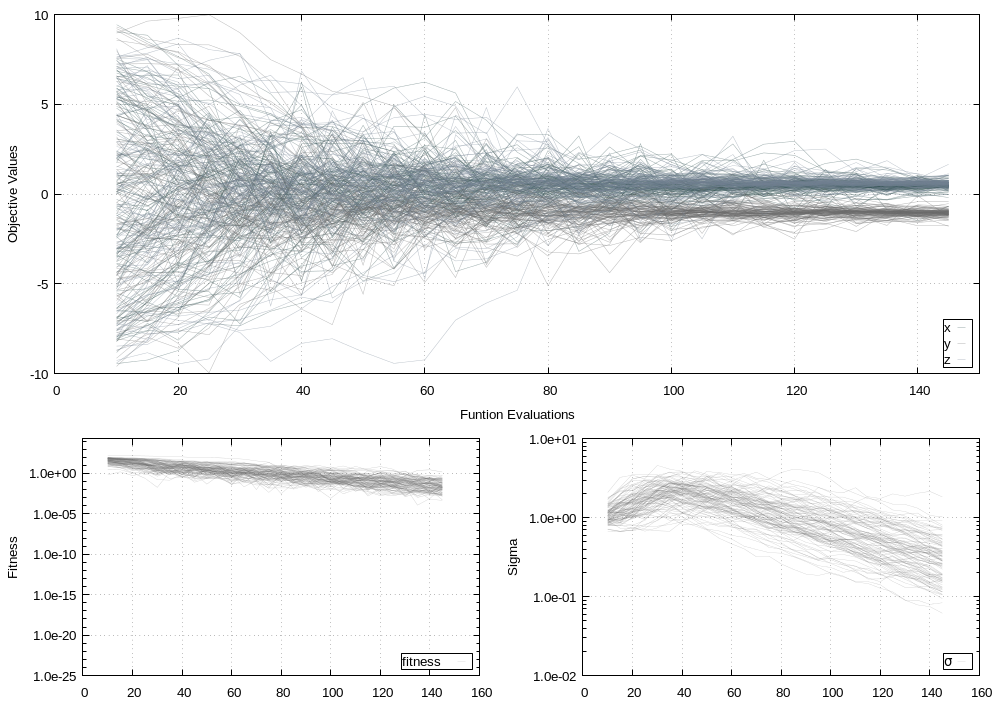
\includegraphics[width=\textwidth]{img/calibration/aborted_calibration_ant0-lines.png}
             \caption{Linienplot der bei $140$ Evaluationen abgebrochenen Verläufe. Gut zu sehen ist der Verlauf der Objektvariablen, die sich von Generation zu Generation dem realen Wert nähern.}
             \label{fig:abortedFinal_Calibration_Ant0_ES-Lines}
     \end{subfigure}
%
\\
%
     \begin{subfigure}[t]{0.4\textwidth}
             \centering
             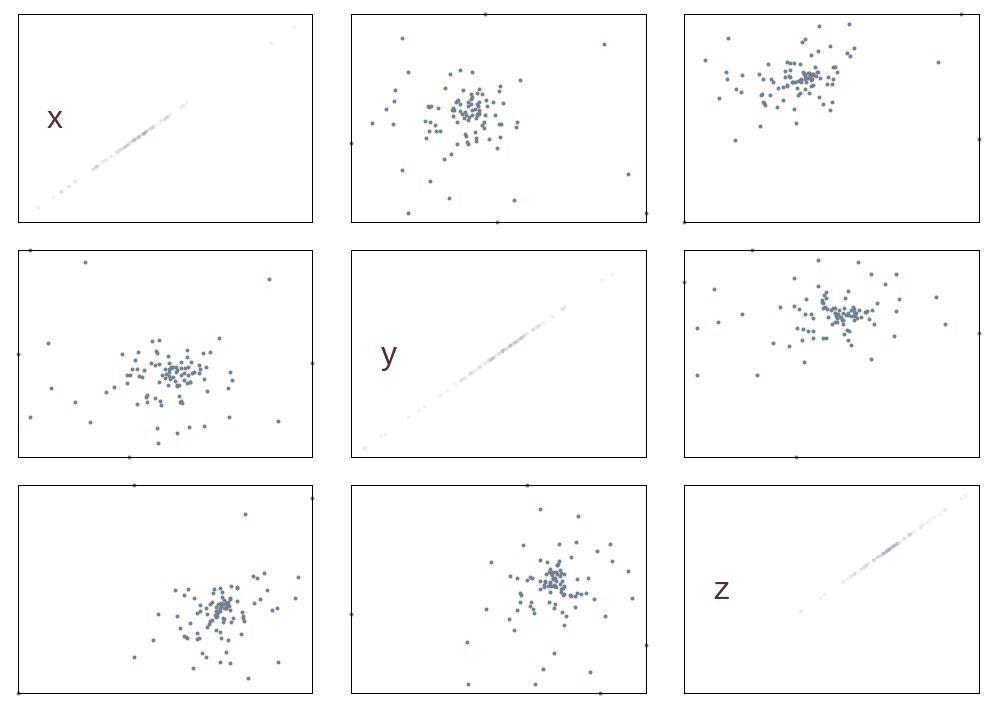
\includegraphics[width=\textwidth]{img/calibration/aborted_calibration_ant0-scatter.png}
             \caption{Statistische Streuung um einen Mittelwert. So in etwa kann man die Lösungen der Komplexen Probleme erwarten.}
             \label{fig:abortedFinal_Calibration_Ant0_ES-Scatter}
     \end{subfigure}
%
     \caption[Statistisch verteilte Ergebnisse der Kalibrierung mittels ES]{Analog zu den Abbildungen~\ref        {fig:abortedFinal_Calibration_Ant0_ES-Lines}, \ref{fig:abortedFinal_Calibration_Ant0_ES-boxes} und \ref{fig:abortedFinal_Calibration_Ant0_ES-Scatter} zeigen die Plots die gleichen Darstellungen. Hier gezeigt wird, wie sich eine statistische Verteilung in den Plots manifestieren würde. Um das zu demonstrieren wurde das Abbruchkriterium auf lediglich $150$ Evaluationen der Zielfunktion eingestellt. Zu diesem Zeitpunkt können die Objektvariablen bereits einen passablen Wert erreicht haben oder noch abweichende Werte aufweisen (vgl. \ref{fig:Final_Calibration_Ant0_ES-Lines}).}
     \label{fig::abortedFinal_Calibration_Ant0_ES}
\end{figure}
%
\begin{figure}[ht!]
         \centering
         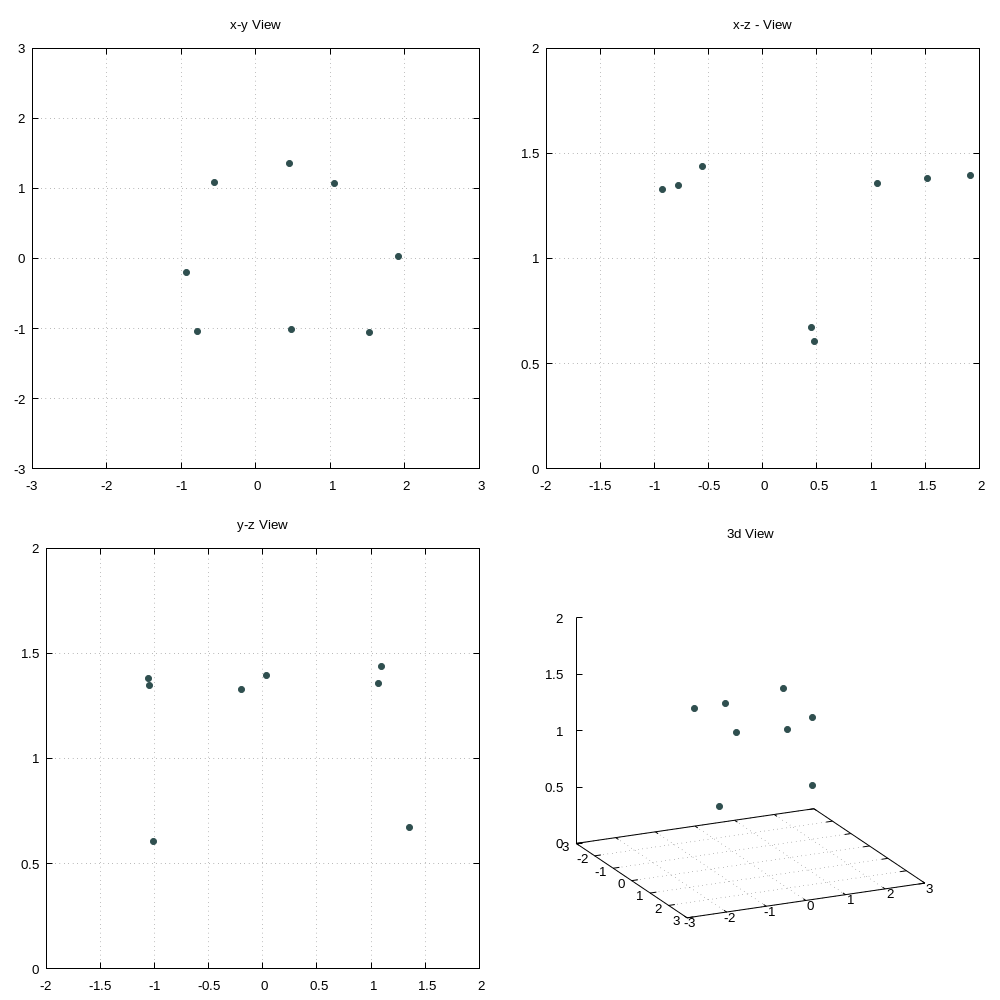
\includegraphics[width=0.7\textwidth]{img/calibration/calibration_results.png}
         \caption[Visualisierung des Kalibrierendergebnis]{Visualisierung des Kalibrierendergebnis. Abgebildet sind die gefundenen Antennenkoordinaten (Punkte) in drei Raumansichten. Die zusätzliche, dreidimensionale  Ansicht dient der Übersicht. Das Ergebnis und die reale Anordnung decken sich sehr gut. Siehe Tabelle~\ref{tab:FinalCoords}}
         \label{fig:3dplot_coordinates}
%
\end{figure}
%
\begin{figure}[ht!]
         \centering
         \caption[Kalibrierwerkzeuge]{Werkzeuge, die bei der Kalibrierung verwendet werden.}
         \begin{subfigure}[t]{0.4\textwidth}
                 \centering
                 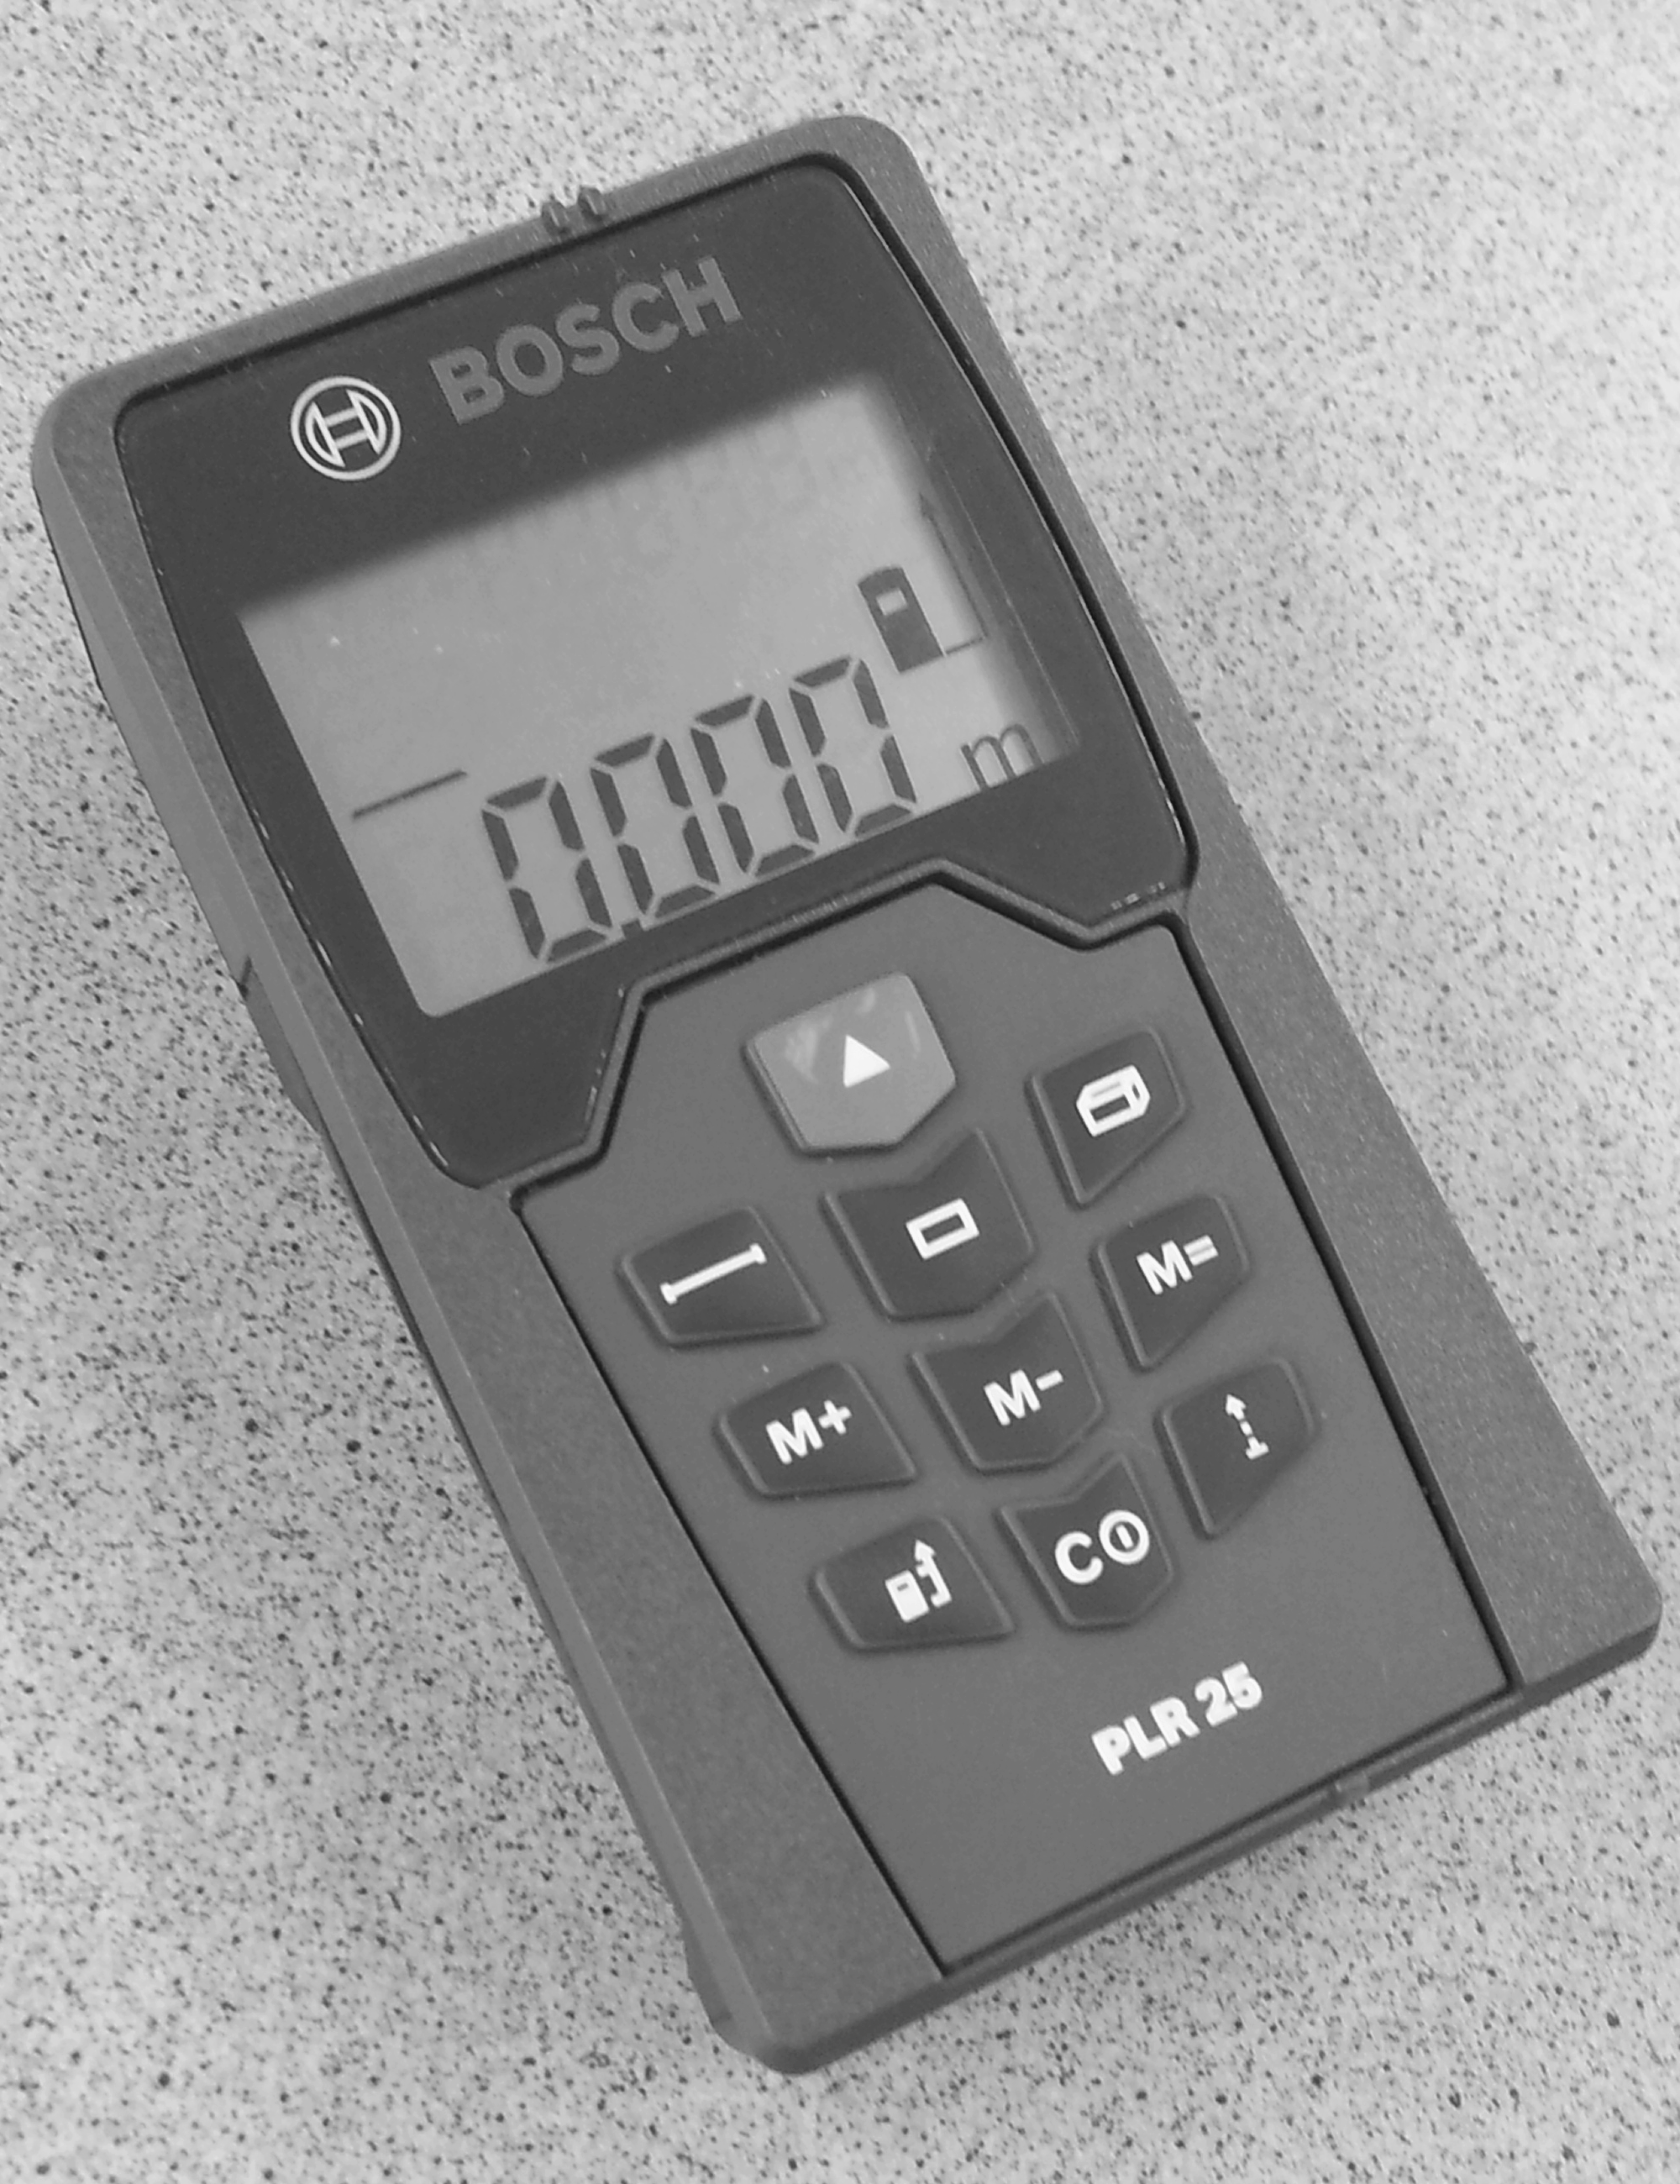
\includegraphics[width=\textwidth]{img/Lasermeter.png}
                 \caption{Laser Distanzmesser}
                 \label{fig:laser_meter}
         \end{subfigure}
%
\qquad         
%
         \begin{subfigure}[t]{0.4\textwidth}
                 \centering
                 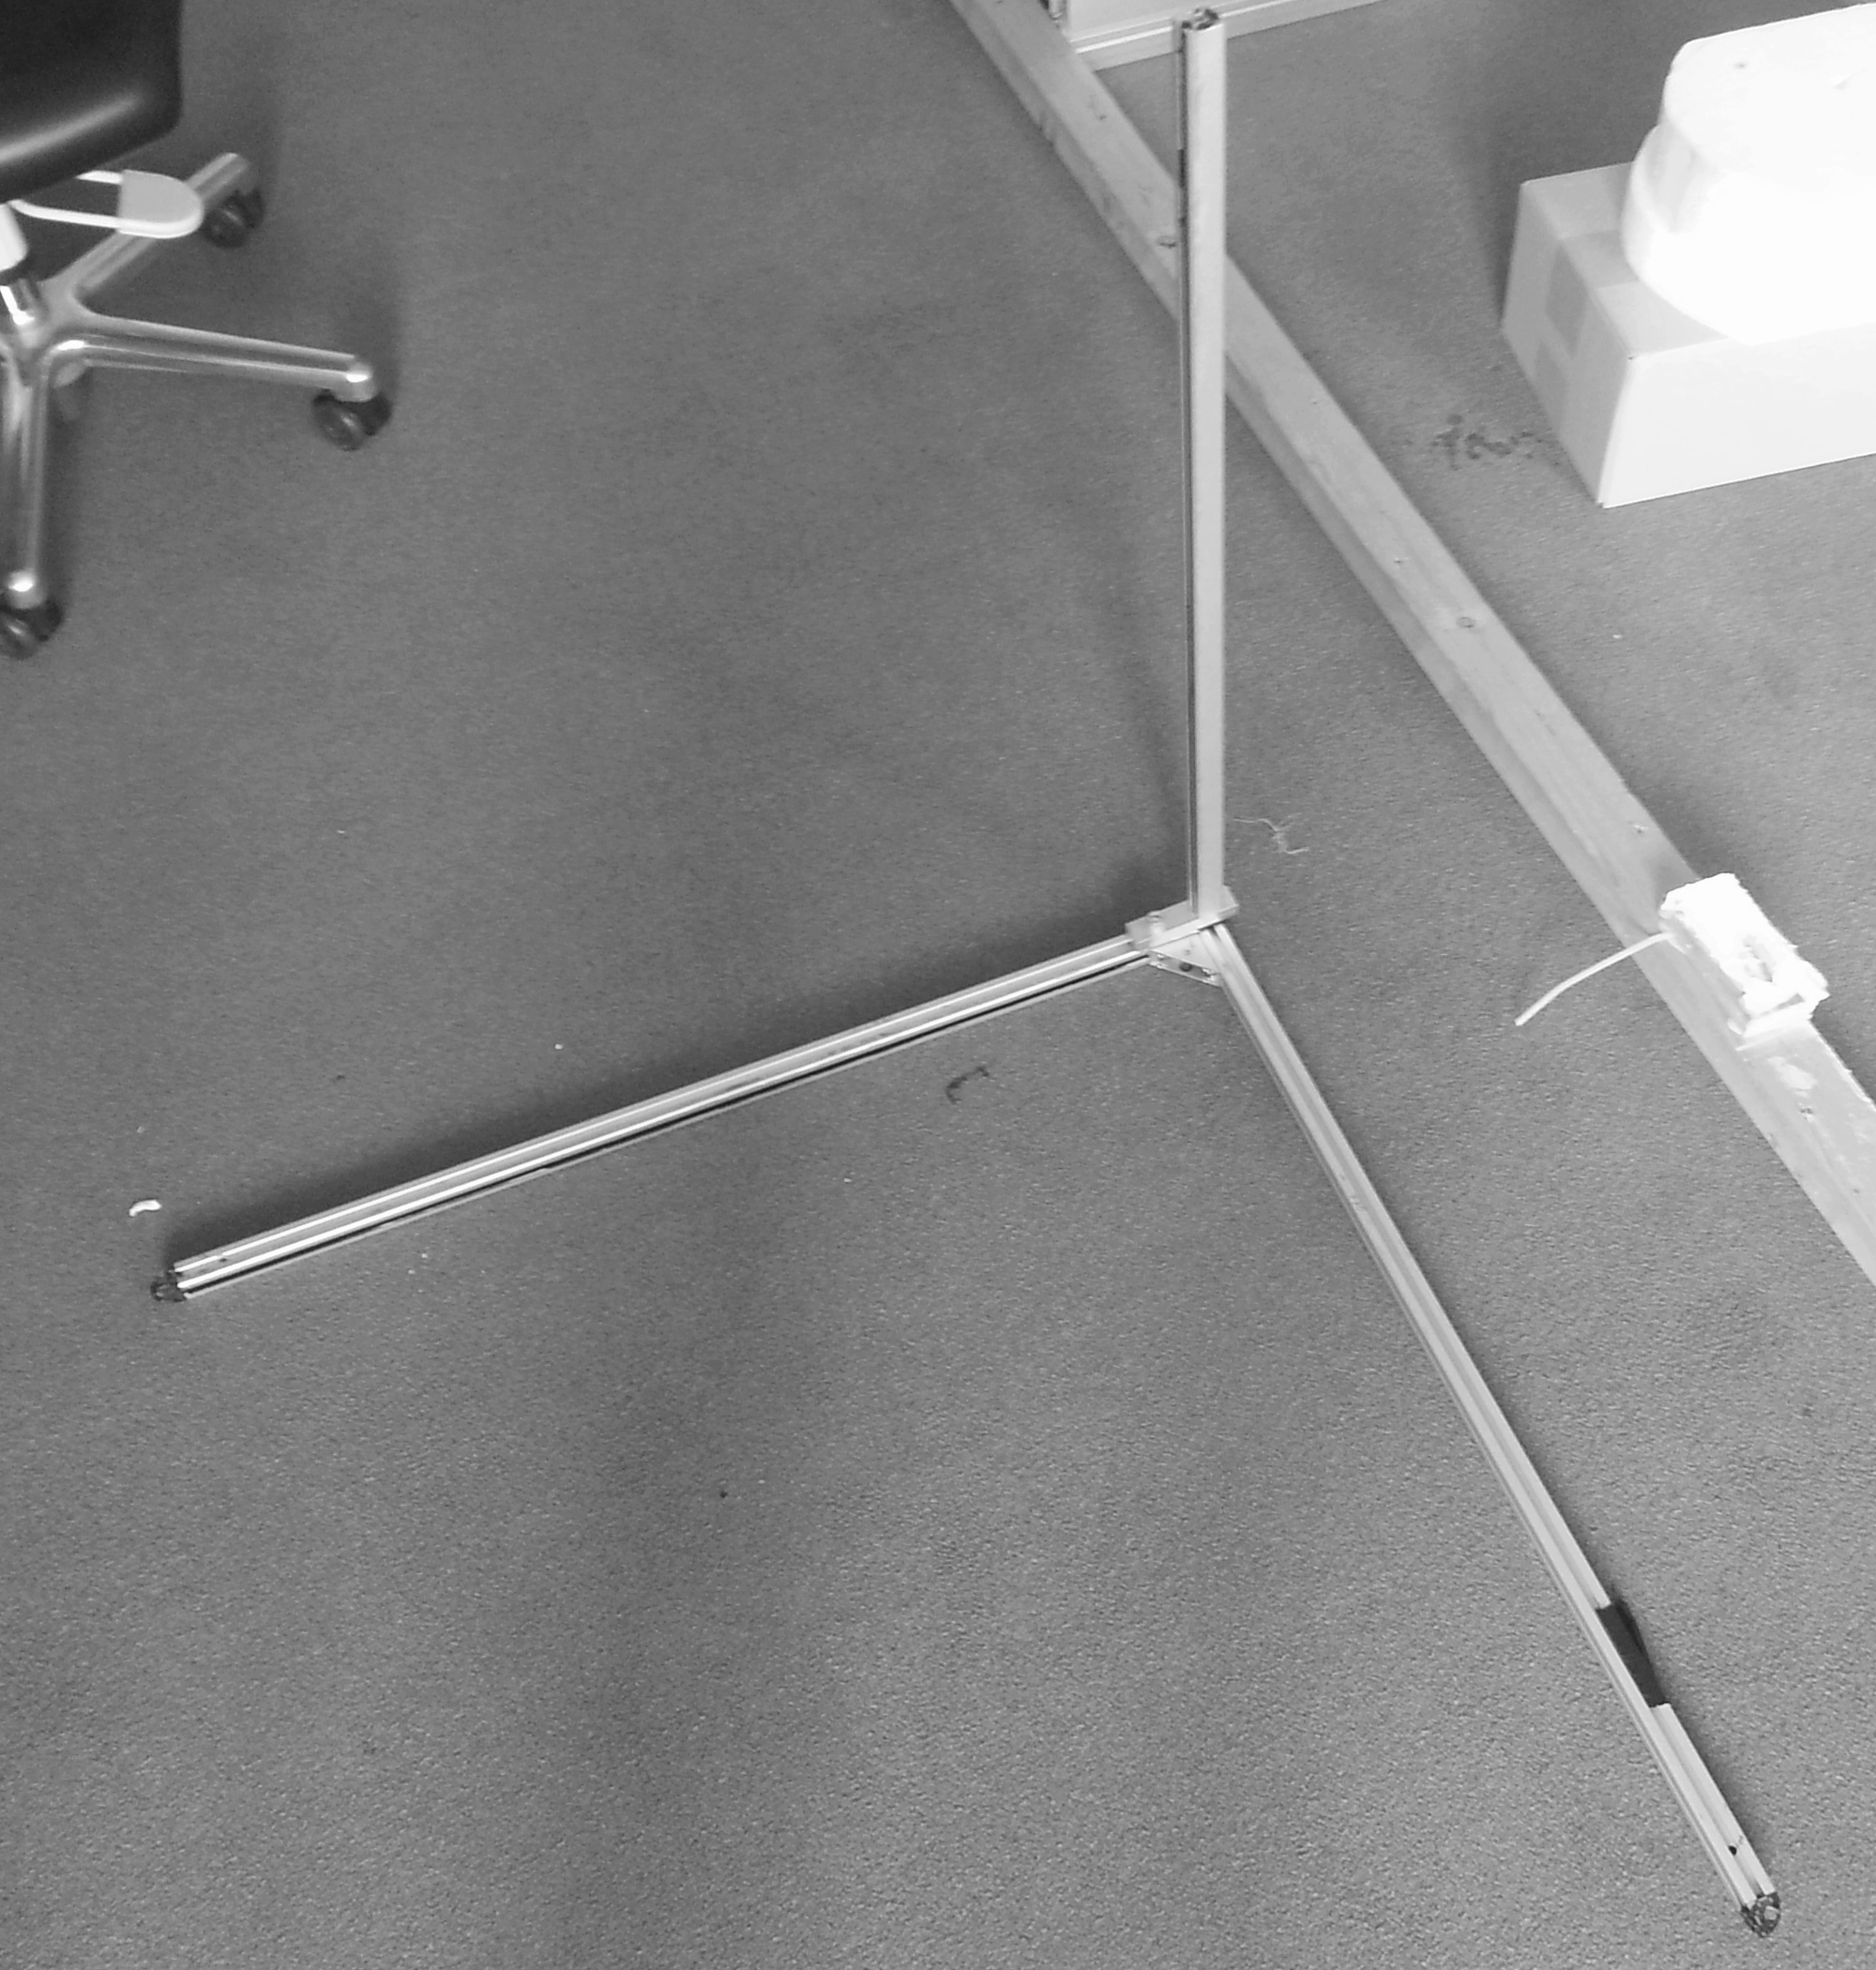
\includegraphics[width=\textwidth]{img/Calibration_Phantom.png}
                 \caption{Kalibrierstück mit vier Messpositionen. }
                 \label{fig:calib_piece}
         \end{subfigure}
         \label{fig:Calibration_Tools}
\end{figure}

%

Das Modell aus \ref{sec:model_developement} wurde in verschiedenen Experimenten untersucht. Dabei wurden die Parameter der Optimierung variiert und die Auswirkungen untersucht.

Es wird analysiert, wie gut die Lösbarkeit des unregistrierten Problems ist. Dazu werden zuerst für jede Referenzantenne immer eine mögliche Konfiguration gewählt und das Ergebnis aus $M$-Durchläufen untersucht. Im Anschluss %MENE: trinken wir Bier! %CG: DAS MACHEN WIR!

Zunächst werden die Ergebnisse der Experimente für idealen Messwerte vorgestellt, dannach wird dieselbe Darstellung für reale Messdaten vorgenommen. Die Darstellung der Ergebnisse ist eine kondensierte Form der Präsentation. Sie Zeigen 
%
%-----------------------------------------------------------------------------
%
\subsection{Experimente}
%
Die Tabellen~\ref{tab:experiments} und~\ref{tab:experiments2} geben an welche Parameter wie variiert wurden. Diese Experimente wurde für die Präsentation der Ergebnisse in dieser Arbeit entworfen. Alle wurden mit der gleichen Objektfunktion durchgeführt. Diese trägt den Namen '\textit{WholeTomatoMkII}'\footnote{Implementation des in dieser Arbeit entwickelten Trilaterationsmodells}. Der eingesetzte Algorithmus ist das CMA-ES. Andere evolutionäre Strategien werden nicht in separaten Experimenten untersucht und präsentiert. Die spätere Darstellung kondensieren die Parameter und Erkenntnisse die in dieser Arbeit gewonnen wurden. Ziel ist es insgesamt die Lösung zu quantifizieren. Wie im Rahmen der Komplexitätsuntersuchung beschrieben ist die Fragestellung die hier bearbeitet wird recht komplex. Es werden daher die Parameter der Evolutionsstrategie variiert. Dabei wird untersucht ob und wie sich die Güte der Lösung durch diese Parameter verbessern lässt. In den Abbildungen~\ref{fig:results1} und~\ref{fig:results2} sind die Ergebnisse der Experimente als Heatmap dargestellt.

%
\begin{table} [H]	
	\label{tab:experiments}
	\caption[Experimente - Ideale Messdaten]{Aufstellung der Experimente die in diesem Abschnitt vorgestellt werden. Die Gruppengröße wird bei jedem Experiment Variiert. Jedes Unterexperiment erhält seinen eigenen Namen. Daher steigt der Name der Experimente bei jedem Eintrag entsprechend der Anzahl der untersuchten Gruppen an. In dieser Untersuchung wurden auch Parameter des Evolutionären Algorithmus variiert. Es werde $\mu$ und $\lambda$ variiert. Der Einfluss der Populations- und Gruppengröße wird damit gleichzeitig untersucht. Es ergeben sich $100$ einzelne Experimente.}
	\begin{center}
		\begin{tabular}{ccccc}
			\textbf{Name} 	& \textbf{Trials $M$} 	& \textbf{Gruppengröße $L$} & \textbf{$\mathbf{\mu}+\mathbf{\lambda}$}\\
			E2000			& 50 				&    1-10		&  (30+100) \\
			E2010			& 50 				&    1-10		&  (40+150) \\
			E2020			& 50 				&    1-10		&  (50+200) \\
			E2030			& 50 				&    1-10		&  (60+250) \\
			E2040			& 50 				&    1-10		&  (70+300) \\			                        
			E2050			& 50 				&    1-10		&  (80+350) \\			                        
			E2060			& 50 				&    1-10		&  (90+400) \\			                        
			E2070			& 50 				&    1-10		&  (100+450) \\			                        
			E2080			& 50 				&    1-10		&  (110+500) \\			                        
			E2090			& 50 				&    1-10		&  (120+550) \\			                        
%			
		\end{tabular}
	\end{center}
\end{table}
%

\begin{table} [H]	
	\label{tab:experiments2}
	\caption[Experimente - Reale Messdaten]{Für bestmögliche Vergleichbarkeit wurden diese Experimente mit den gleichen Parametern durchgeführt wie die für ideale Daten.}
	\begin{center}
		\begin{tabular}{ccccc}
			\textbf{Name} 	& \textbf{Trials $M$} 	& \textbf{Gruppengröße $L$} & \textbf{$\mathbf{\mu}+\mathbf{\lambda}$}\\
			E3000			& 50 				&    1-10		&  (30+100) \\
			E3010			& 50 				&    1-10		&  (40+150) \\
			E3020			& 50 				&    1-10		&  (50+200) \\
			E3030			& 50 				&    1-10		&  (60+250) \\
			E3040			& 50 				&    1-10		&  (70+300) \\			                        
			E3050			& 50 				&    1-10		&  (80+350) \\			                        
			E3060			& 50 				&    1-10		&  (90+400) \\			                        
			E3070			& 50 				&    1-10		&  (100+450) \\			                        
			E3080			& 50 				&    1-10		&  (110+500) \\			                        
			E3090			& 50 				&    1-10		&  (120+550) \\			                        
%			
		\end{tabular}
	\end{center}
\end{table}
%
%-----------------------------------------------------------------------------
%
\subsection{Ergebnisse ideale Messwerte}
%
\begin{figure}[h!]
	\centering
	\caption[Ergebnis-Heatmap - Idealisierte Werte]{ Ergebnisse verschiedener Experimente. Die Abbildung zeigt farbkodiert den Betrag der Abweichung vom wahren Wert der Entfernung (Ausgemessen). Zu beachten gilt, dass die Farbskala eine unterschiedliche Skalierung hat und somit jede Antenne separat betrachtet werden muss. Die Parameter die in diesen Experimenten variiert wurden sind die Populationsgröße ($\mu$ und $\lambda$) und die Gruppengröße $L$. Mit der $x$-Achse steigt die Populationsgröße an. Die $y$-Achse trägt die steigende Gruppengrößen auf.}
	\label{fig:results1}
	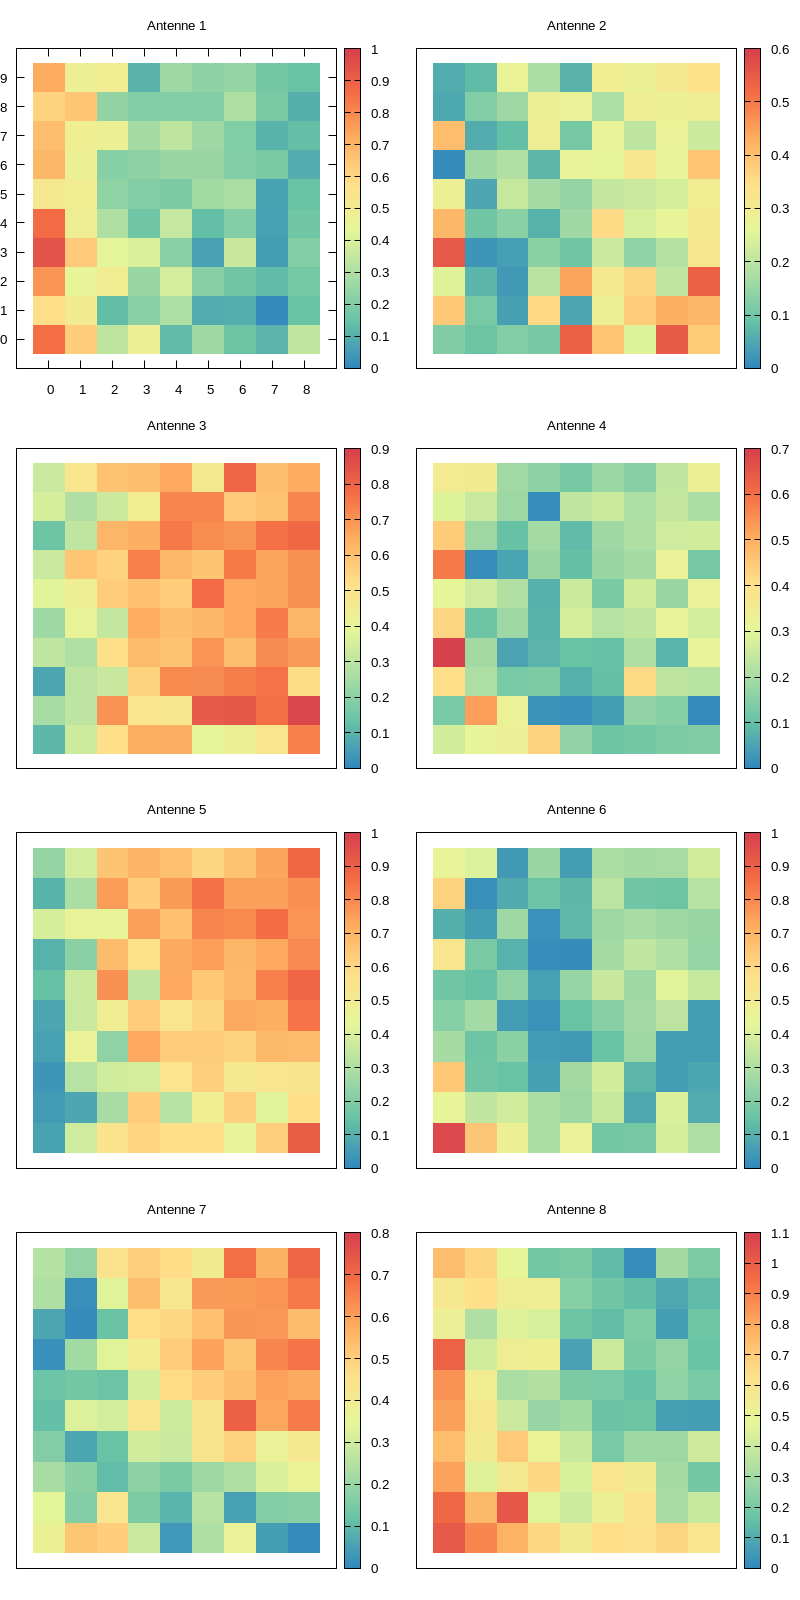
\includegraphics[width=0.65\textwidth]{img/result.png}
\end{figure}
% 
Um die idealen Messwerte zu generieren wurde ein eigenes Modul entwickelt. Es verwendet die in Kapitel~\ref{sec:PhaseCalculation} beschrieben Formeln. Es wurden eine Reihe von Punkten definiert, von denen die idealen Phasenwerte ermittelt wurden. Um im Rahmen dieser Arbeit in der Präsentation der Ergebnisse konsistent zu bleiben, wird als Punkt der Ursprung der Kalibrierung genutzt. Dieser muss von dem Algorithmus wiedergefunden werden. Seine Koordinaten wurden bereits in Kapitel~\ref{sec:calibration} besprochen. Die in den Abbildungen gezeigte Darstellung stellt die Abweichung von dem korrekten Wert dar.
$$
\varepsilon=~|~d_{true}-d_{found}~|
$$
Die Dimension von $\varepsilon$ ist dementsprechend [m].
%
\subsection{Ergebnisse ideale Messwerte}
%
Die idealen Messewerte zeigen insgesamt ein gutes Ergebnis. Im Mittel werden die Besten Ergebnisse, bei mittlerer Gruppengröße und großer Populationsgröße gefunden. Es zeigt sich, dass eine steigende Populationsgröße das Ergebnis in der Regel verbessert. Bei der Gruppengröße kann ab einer bestimmten Größe keine weitere Verbesserung festgestellt werden. Eine Besonderheit zeigt sich bei den Antennen $3$ und $5$. Diese zeigen ein umgekehrtes Verhalten, bei niedriger Gruppengröße und kleiner Populationsgröße zeigen sie die geringste Abweichungen. Woran das liegt konnte nicht weiter untersucht werden. Die meisten Lösungen zeigen eine Abweichung von unter einer Wellenlänge, die wir mit $\lambda\simeq35$~cm angeben konnten. Das erlaubt prinzipiell eine korrekte Berechnung der Wellenzahl.
%
%-----------------------------------------------------------------------------
%
\subsection{Ergebnisse reale Messwerte}
%
\begin{figure}[h!]
	\centering
	\caption[Ergebnis-Heatmap - Messwerte]{Die Antennen $2$ und $6$ lieferten bei dieser Messung keine Messdaten. Daher fehlen diese Plots in der Grafik. Das Antennen keine Daten liefern ist der Regelfall den man in der Praxis begegnet. }
	\label{fig:results2}
	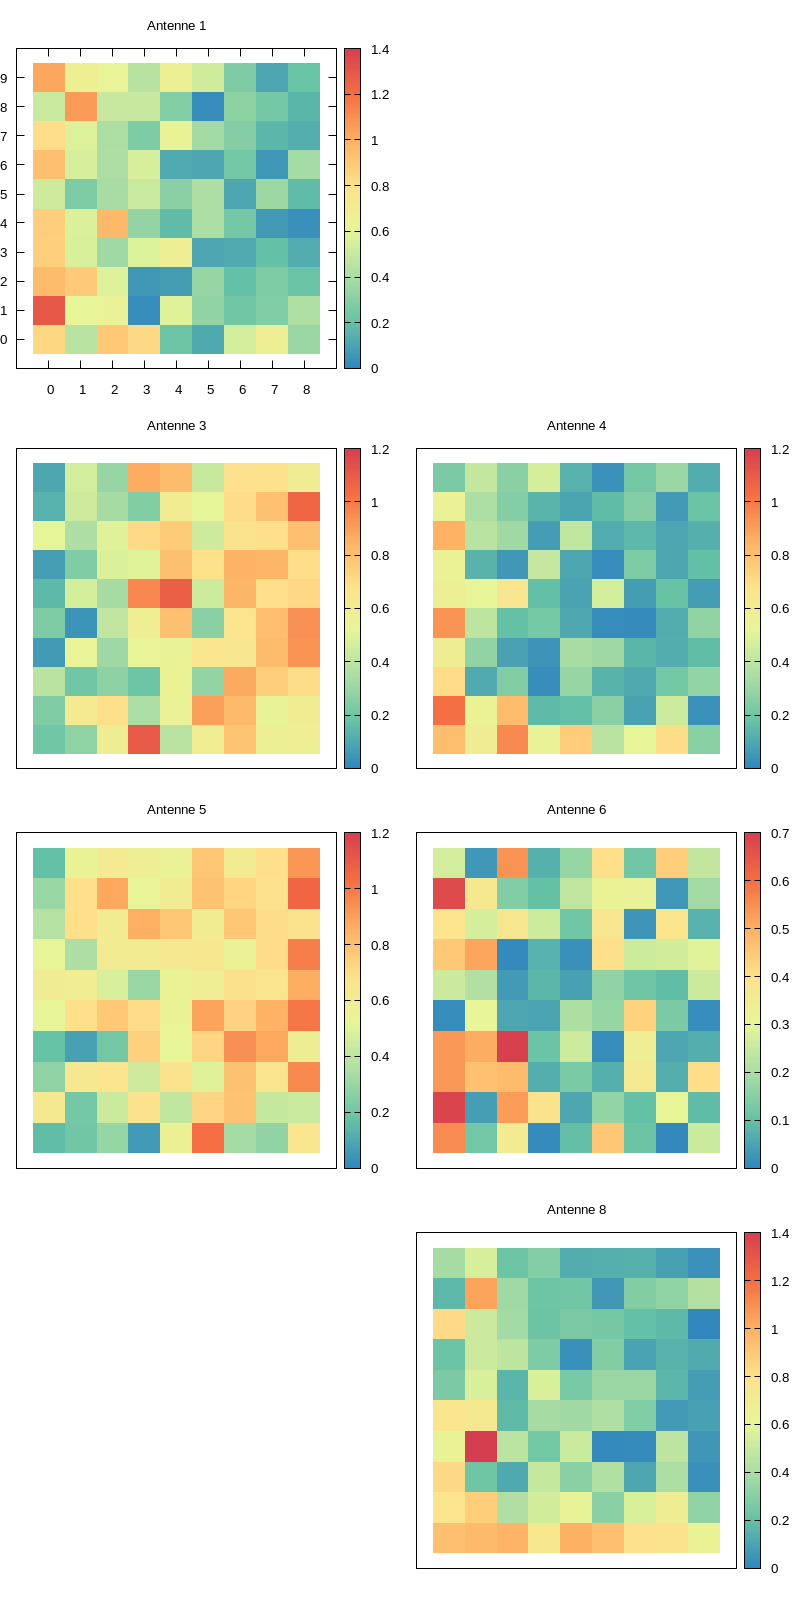
\includegraphics[width=0.65\textwidth]{img/resultRealData.png}
\end{figure}
%
Die Ergebnisse für reale Messwerte zeigen ein ähnliches Bild wie die idealen Messwerte. Eine steigende Gruppen- und Populationsgröße verbessert das Ergebnis in der Regel. Es fehlen die Plots der Antenne $2$ und $6$. Das liegt daran, dass diese beiden Antennen keine Messdaten lieferten. Es wurde der selbe Punkt ausgewählt, wie bei Vorstellung der ideal Messergebnisse. Damit sind die Ergebnisse unmittelbar vergleichbar. Genau wie bei den idealen Messdaten wurde der Ursprung der Kalibrierung als Messpunkt genommen. Das Ergebnis der realen Messwerte mutet sogar sicherer an, als das der idealen Phasenwerte. Der Grund dafür kann nicht exakt angegeben werden. Man kann sich dazu überlegen, da jeder Messwert ein Messrauschen enthält. Dieses Rauschen wird Teil des Modell und variiert dadurch unmittelbar die Fitnesslandschaft. Das Aussehen der Fitnesslandschaft wurde in Kapitel~\ref{sec:Komplexity2} untersucht. Weitere Untersuchungen und größere Messreihen müssen dieses Verhalten bestätigen. 
%
%-----------------------------------------------------------------------------
%
\subsection{Evolutionsverlauf - real vs ideal}
%
Abschließend ist in Abbildung~\ref{fig:results3} der Verlauf der letzten beiden Experimente $2099$ und $3099$ gezeigt. Dort werden in $3$ Plots die Lösungen charakterisiert und die statistischen Eigenschaften sowie der Verlauf der Optimierung quantifiziert. Zu erkennen ist, dass sie die beiden Ergebnisse grundsätzlich ähneln. Unterschiede zeigen sich nur in Einzelheiten, so zeigt sich z.B., dass die Streuung der Parameter bei idealen Messwerten geringer, jedoch mehr Evaluationen notwendig waren. Allgemein zeigt sich der erwartete Verlauf einer evolutionären Optimierung.
%
\begin{landscape}
\begin{figure}[!ht]
	\caption[Evolutionsverlauf der Ergebnisse]{ Diese Grafik zeigt den Verlauf der Evolution. Es werden die Beiden letzten Experimente $2099$ (opben, ideale Messdaten) und $3099$ (unten, reale Messdaten) gezeigt. Diese Plots dienen nur der Einschätzung über den generellen Verlauf der Evolution. Es ist nicht sinnvoll sie für alle Experimente hier darzustellen. Anhand des Boxplots (Mitte) erkennend man, dass die Resultate für ideale Messwerte nicht so stark streuen, die Lösung der realen Messdaten ist den der idealen mind. Ebenbürtig. Es zeigt sich sogar, dass weniger Evaluationen der Zielfunktion bei den realen Werten nötig waren.}
	\label{fig:results3}
	\vspace{3mm}
	\centering
	\begin{subfigure}[t]{0.45\textheight}
	     \centering
	     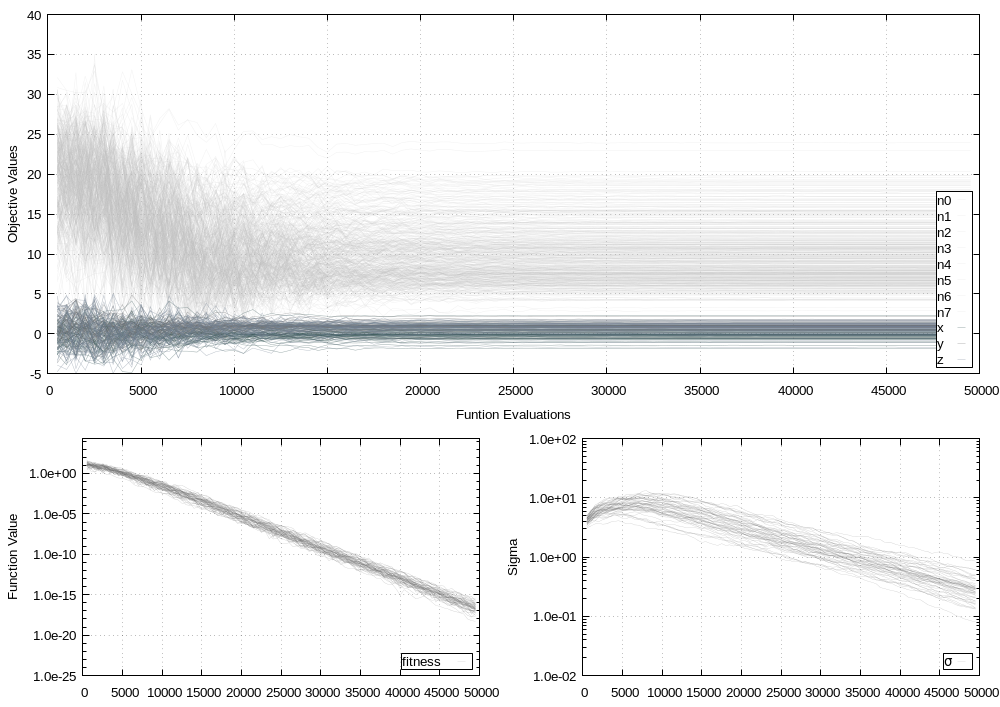
\includegraphics[width=\textwidth]{img/evo/lines2089.png}
	             \caption{Linienplot zur Analyse der Variablen und Optimierungsverlaufs.}
	%             \label{fig:abortedFinal_Calibration_Ant0_ES-boxes}
	\end{subfigure}
	\qquad
	\begin{subfigure}[t]{0.45\textheight}
		\centering
	     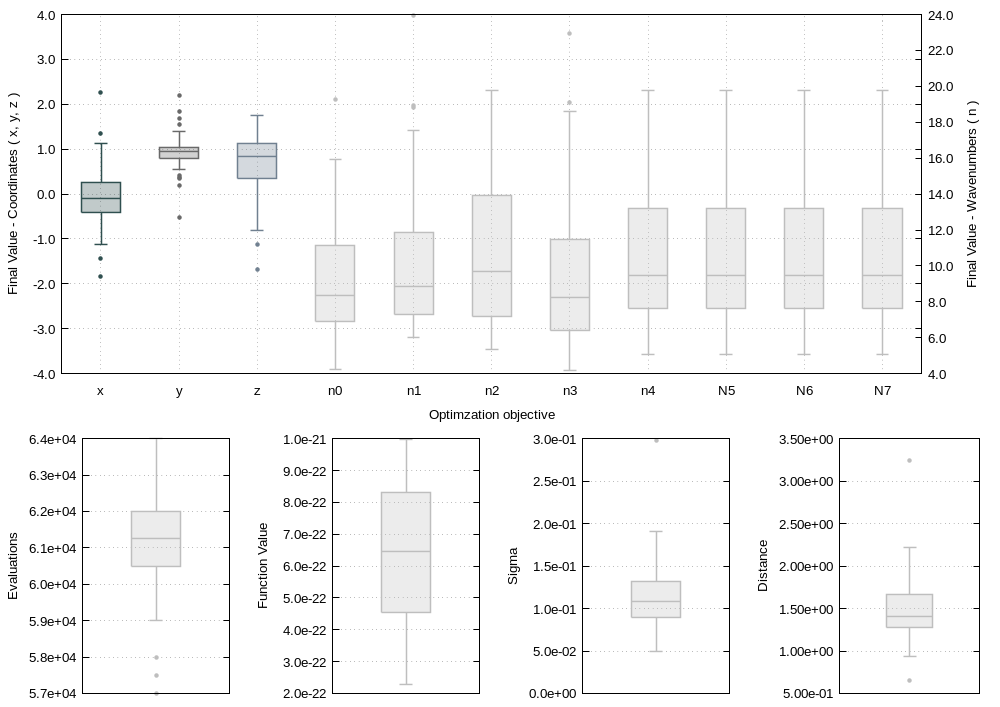
\includegraphics[width=\textwidth]{img/evo/boxes2089.png}
	     	    \caption{Boxplot zur Veranschaulichung der Lösungsstatistik }
	%			\label{fig:abortedFinal_Calibration_Ant0_ES-boxes}
	\end{subfigure}
	\qquad
	\begin{subfigure}[t]{0.45\textheight}
			\centering
	   \includegraphics[width=\textwidth]{img/evo/Scatter2089.png}
	   	       \caption{Streuplot zur Untersuchung von Abhängigkeiten der Parameter}
	%			\label{fig:abortedFinal_Calibration_Ant0_ES-boxes}
	\end{subfigure}
	\vspace{5mm}
\\
	\centering
	\begin{subfigure}[t]{0.45\textheight}
	     \centering
	     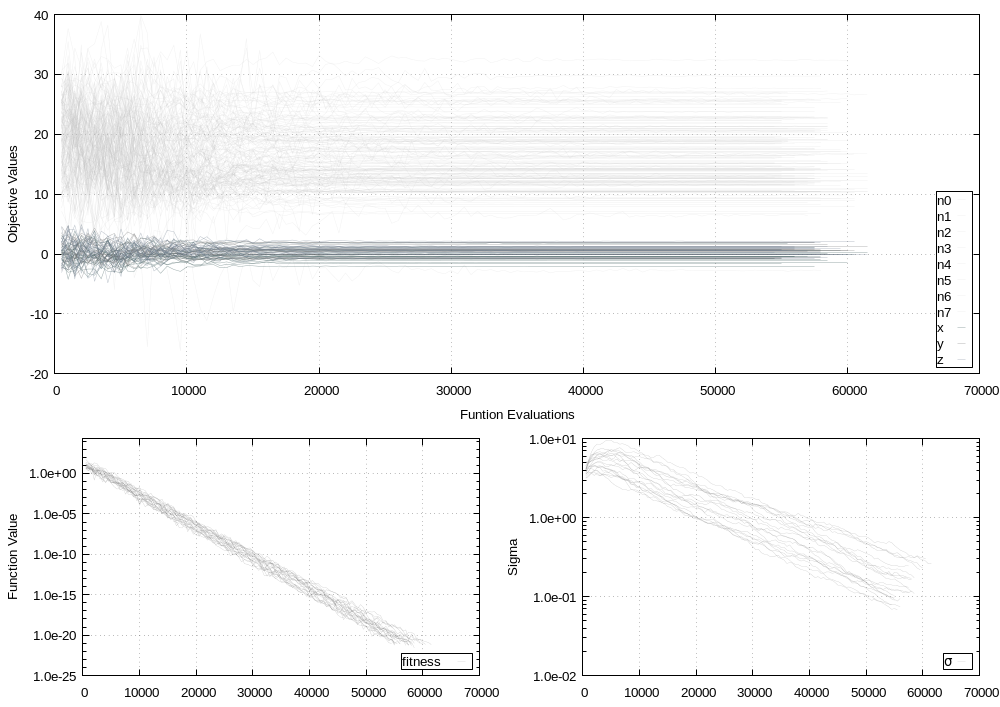
\includegraphics[width=\textwidth]{img/evo/lines4089.png}
	             \caption{Linienplot zur Analyse der Variablen und Optimierungsverlaufs.}
	%             \label{fig:abortedFinal_Calibration_Ant0_ES-boxes}
	\end{subfigure}
	\qquad
	\begin{subfigure}[t]{0.45\textheight}
		\centering
	     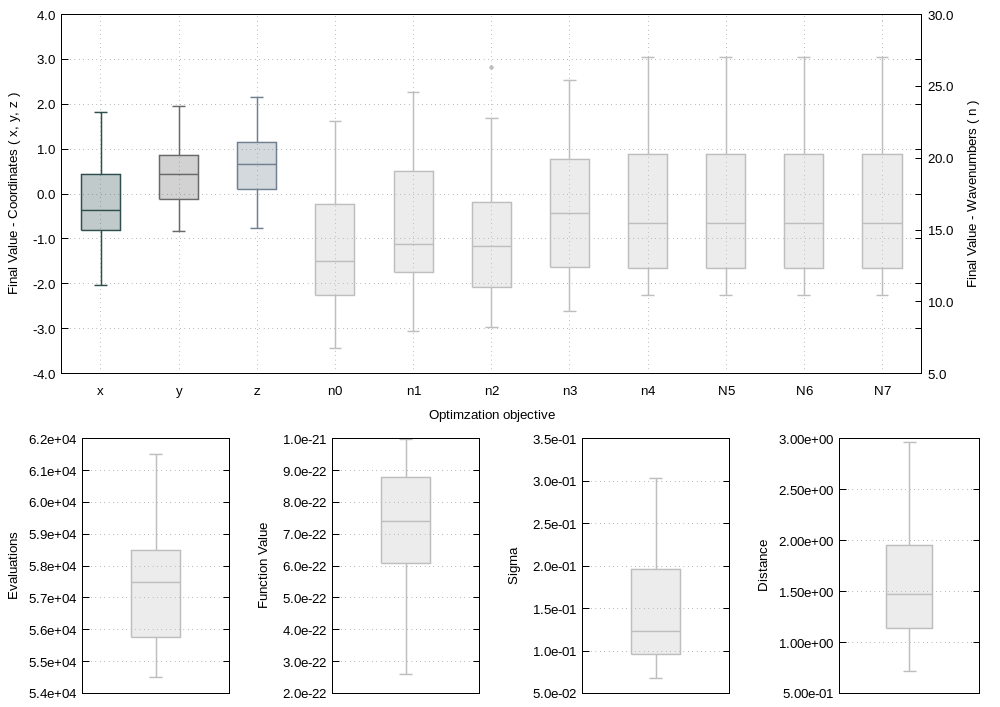
\includegraphics[width=\textwidth]{img/evo/boxes4089.png}
	     	    \caption{Boxplot zur Veranschaulichung der Lösungsstatistik }
	%			\label{fig:abortedFinal_Calibration_Ant0_ES-boxes}
	\end{subfigure}
	\qquad
	\begin{subfigure}[t]{0.45\textheight}
			\centering
	   \includegraphics[width=\textwidth]{img/evo/Scatter4089.png}
	   	       \caption{Streuplot zur Untersuchung von Abhängigkeiten der Parameter}
	%			\label{fig:abortedFinal_Calibration_Ant0_ES-boxes}
	\end{subfigure}

\end{figure}
\newpage
\end{landscape}

%

%
% 4. ------------------------------------------------------------------------
\chapter{Diskussion}
Vergleich der Ergebnisse mit den Zielen der Arbeit.\\
%
\lipsum[1-5]
%
Die in dieser Arbeit erreichten Ergebnisse erfüllen die
%
% 5. ------------------------------------------------------------------------
\chapter{Schluss}
\lipsum[1-2]

\section{Offene Punkte}
\section{Diskussion der Ergebnisse}
\lipsum[1-3]
\section{Verbesserungen}
\section{Ausblick}
%
%----------------------------------------------------------------------------
% Appendix ------------------------------------------------------------------
%----------------------------------------------------------------------------
%
%
%
\begin{appendix}

%----------------------------------------------------------------------------
%----------------------------------------------------------------------------
%\newpage
%
%\begin{center}
%	\huge{Anhänge}
%\end{center}

\normalsize
%
%----------------------------------------------------------------------------
%----------------------------------------------------------------------------
\chapter{Abbildungen}
\section{Messaufbauten}
\begin{figure}[h!]
 \centering
         \includegraphics[width=\textwidth]{img/00_Placeholder.png}
         \caption[PRPS-Kalibiersystem]{PRPS-Messsystem in der "Spinnen"-Konfiguration. Es umfasst vier Messwertgeber und eine Recheneinheit.}
         \label{fig:Spider1}
\end{figure}
\newpage
%
%----------------------------------------------------------------------------
%----------------------------------------------------------------------------
\begin{figure}[h!]
 \centering
         \includegraphics[width=\textwidth]{img/00_Placeholder.png}
         \caption[Übersicht Kalibrieraufbau]{Aufbau des für die Kalibrierung verwendeten Messaufbaus.}
         \label{fig:Spider_setup1}
\end{figure}
\newpage
%
%----------------------------------------------------------------------------
%----------------------------------------------------------------------------
\chapter{Gnuplot Skripte}
\section{Boxplot}
\tiny
\lstinputlisting[
		title=Gnuplot Boxplot-Skript,
		caption=Gnuplot Boxplot-Skript,
		language=Gnuplot,
		numbers=left,
%		frameround=fttt,
		frame=trbl,
		breakatwhitespace=false,         % sets if automatic breaks should only happen at whitespace
   	    breaklines=true,  
		xleftmargin=1cm,
		showstringspaces=false]{../../dev/src/c-cpp/AntConfApp/build/Debug/test/output/mkII/plot/kondensierte_boxen.gp}
\label{append_Script_Box-plot}
\newpage
%
%----------------------------------------------------------------------------
%----------------------------------------------------------------------------
\section{Lineplot}
%\begin{footnote}
\tiny 
%
% listings print source code

% define colors for source code list
\definecolor{colKeys}{rgb}{0,0,1}
\definecolor{colIdentifier}{rgb}{0,0,0}
\definecolor{colComments}{rgb}{0,1,0.3}
\definecolor{colString}{rgb}{0,0.5,0}

\definecolor{dkgreen}{rgb}{0,0.6,0}
\definecolor{gray}{rgb}{0.5,0.5,0.5}

\lstset{language=Matlab,
   keywords={break,case,catch,continue,else,elseif,end,for,function,
   global,if,otherwise,persistent,return,switch,try,while,ones,zeros},
   float=hbp,
   basicstyle=\ttfamily\small,
   identifierstyle=\color{colIdentifier},
   keywordstyle=\color{blue},
   commentstyle=\color{dkgreen},
   stringstyle=\color{red},
   columns=flexible,
   tabsize=2,
   frame=single,
   numbers=left,
   extendedchars=true,
   showspaces=false,
   numberstyle=\tiny\color{gray},
   stepnumber=1,
   numbersep=10pt,
   showspaces=false,
   showstringspaces=false,
   breakautoindent=true}

\lstinputlisting[
		title=Gnuplot Lineplot-Skript,
		caption=Gnuplot Lineplot-Skript,
		language=Gnuplot,
		numbers=left,
%		frameround=fttt,
		frame=trbl,
		breakatwhitespace=false,         % sets if automatic breaks should only happen at whitespace
   	    breaklines=true,  
		xleftmargin=1cm,
		showstringspaces=false]{../../dev/src/c-cpp/AntConfApp/build/Debug/test/output/mkII/plot/kondensierte_linien.gp}
\label{append_Script_Line-plot}
\newpage
%
%----------------------------------------------------------------------------
%----------------------------------------------------------------------------
\section{Scatterplot}
%\begin{footnote}
%
% listings print source code

% define colors for source code list
\definecolor{colKeys}{rgb}{0,0,1}
\definecolor{colIdentifier}{rgb}{0,0,0}
\definecolor{colComments}{rgb}{0,1,0.3}
\definecolor{colString}{rgb}{0,0.5,0}

\definecolor{dkgreen}{rgb}{0,0.6,0}
\definecolor{gray}{rgb}{0.5,0.5,0.5}

\lstset{language=Matlab,
   keywords={break,case,catch,continue,else,elseif,end,for,function,
   global,if,otherwise,persistent,return,switch,try,while,ones,zeros},
   float=hbp,
   basicstyle=\ttfamily\small,
   identifierstyle=\color{colIdentifier},
   keywordstyle=\color{blue},
   commentstyle=\color{dkgreen},
   stringstyle=\color{red},
   columns=flexible,
   tabsize=2,
   frame=single,
   numbers=left,
   extendedchars=true,
   showspaces=false,
   numberstyle=\tiny\color{gray},
   stepnumber=1,
   numbersep=10pt,
   showspaces=false,
   showstringspaces=false,
   breakautoindent=true}

\tiny
\lstinputlisting[
		title=Gnuplot Scatterplot-Skript,
		caption=Gnuplot Scatterplot-Skript,
		language=Gnuplot,
		numbers=left,
%		frameround=fttt,
		frame=trbl,
		breakatwhitespace=false,         % sets if automatic breaks should only happen at whitespace
   	    breaklines=true,  
		xleftmargin=1cm,
		showstringspaces=false]{../../dev/src/c-cpp/AntConfApp/build/Debug/test/output/mkII/plot/scatter.gp}
\label{append_Script_Scatter-plot}
\newpage
%
%----------------------------------------------------------------------------
%----------------------------------------------------------------------------
%\section{Filter Entwurf - Ergebnisse}
%\begin{landscape}
%\label{FirFilterResult}
%\begin{figure} [h]
         \centering
         \caption{ Ergebnisse des Filterentwurfs }
         \label{fig:1}
         \centering
         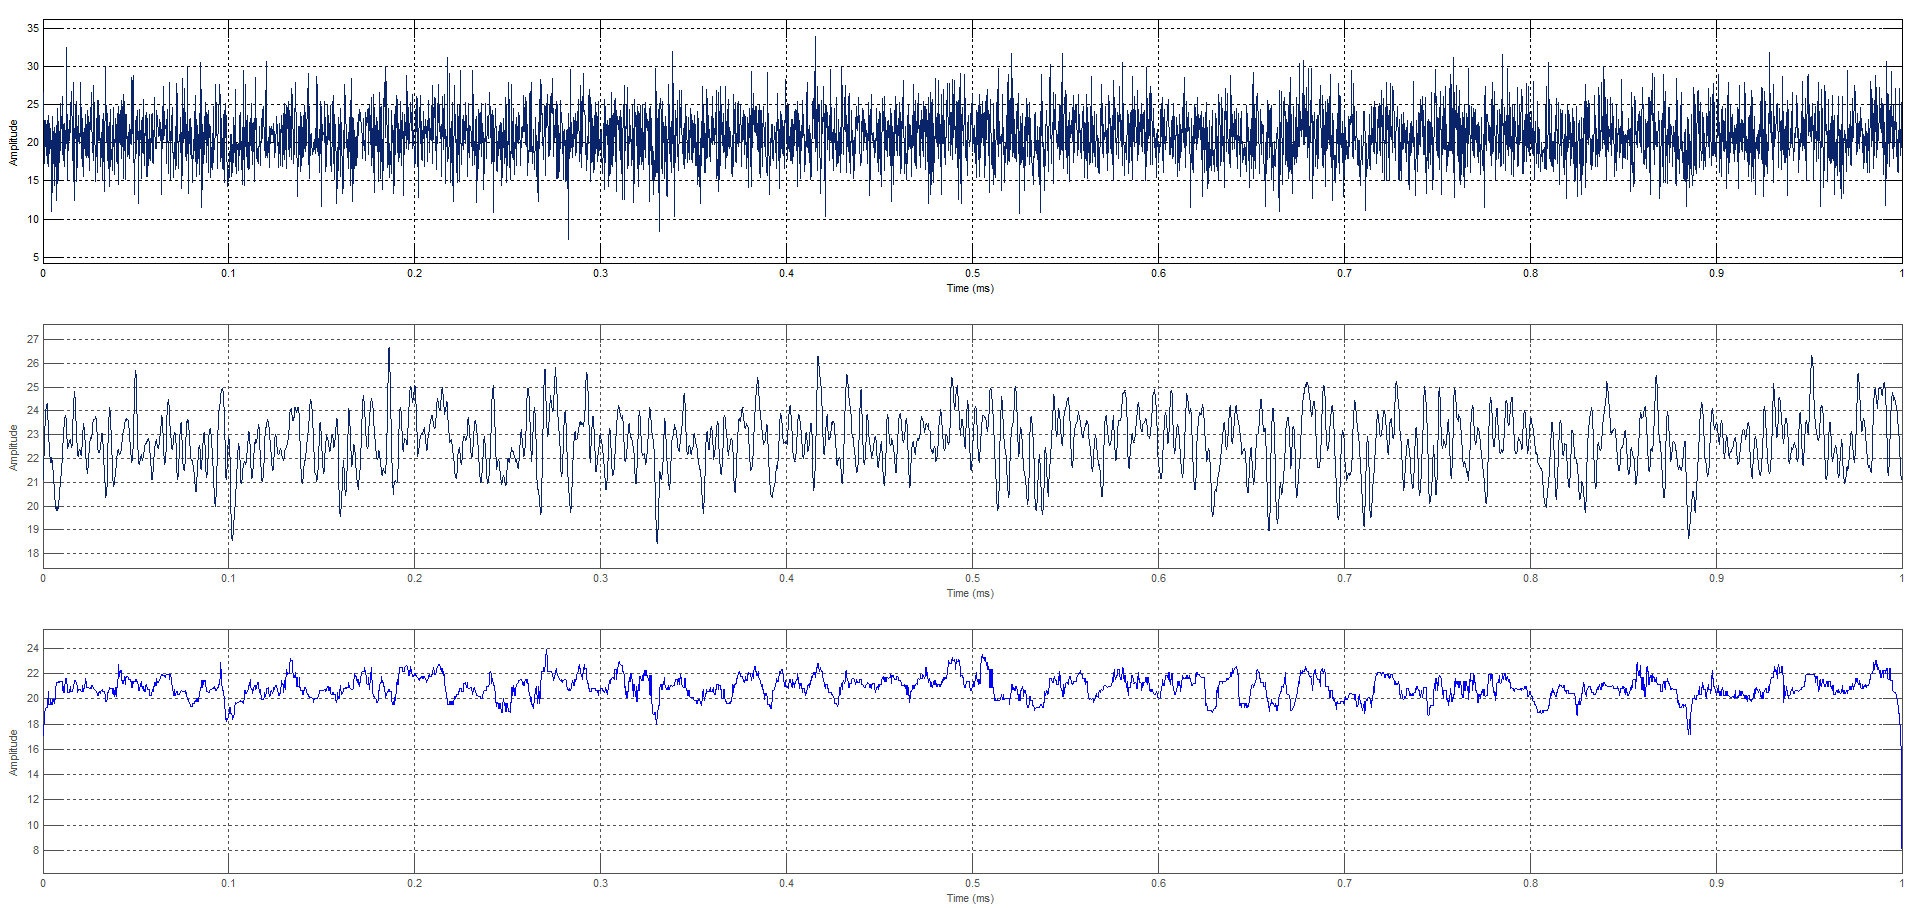
\includegraphics[width=.8\textwidth]{common/img/AmpGefiltert_small.png}\\
\vspace{0.5cm}
Die obere Kurve visualisiert die Rohdaten. Die mittlere Kurve ist das Ergebnis der Tiefpassfilterung für einen der vorgestellten Filter. Die untere Darstellung dient zum Vergleich mit der bisher eingesetzten Filterungsmethode (Median). Es wurden 4096 Messwerte für diese Analyse gesampelt.
\end{figure}
%---------------------------------------------------------------------------------------
\vspace{.5cm}
%---------------------------------------------------------------------------------------
\begin{figure} [h]
         \centering
         \caption{ Spektrum des Messsignals, vor und nach der Filterung  }
         \label{fig:2}
	     \centering
	     \includegraphics[width=.6\textwidth]{common/img/SpektrumAmp.PNG} \\
\vspace{.2cm}
Die Grafik zeigt das Spektrum des Messsignals der Amplitude. Im linken Bild ist das ungefilterte Signal und im Rechten das gefilterte.
%
\end{figure}
%---------------------------------------------------------------------------------------
\vspace{.5cm}
%---------------------------------------------------------------------------------------
\begin{figure} [h]
         \centering
         \caption{ Frequenzgänge der entworfenen Filter. Beide ähneln sich in den Parametern, verfügen jedoch über etwas unterschiedliche Eckfrequenzen. Als Entwurfsmethode wurde die sog. "Least-squares"-Methode verwendet. Diese Methode liefert gute Ergebnisse im Hinblick auf möglichst kleine Sidelobes und eine geringe Anzahl an Koeffizienten. }
         \label{fig:3}
%         
         \begin{subfigure}[t]{0.5\textwidth}
                 \centering
                 \includegraphics[width=\textwidth]{common/img/filter.png}
                 \vspace{.1cm}
                 \caption{Erstes Filter mit den Parametern wpass~=~0.1 und wstop~=~0.15. Das Ergebnis ist ein schmalbandigeres Filter. }
                 \label{fig:Filter1_A}\textit{}
         \end{subfigure}
%         
\qquad
         \begin{subfigure}[t]{0.5\textwidth}
                 \centering
                 \includegraphics[width=\textwidth]{common/img/filter2.png}
                 \vspace{.1cm}
                 \caption{ Zweites Filter mit den Parametern wpass~=~0.1 und wstop~=~0.2. Der Durchlas bereich ist etwas breiter, dafür sind die Sidelobes stärker gedämpft }
                 \label{fig:Filter2_B}
         \end{subfigure}
%
\end{figure}
%---------------------------------------------------------------------------------------
%\end{landscape}
%
%----------------------------------------------------------------------------
%----------------------------------------------------------------------------
%\newpage
%\begin{landscape}
%	\section{Projektlaufplan KW 31}
%	\label{sec:projectplan}
%	\scalebox{.75}{
%		\begin{ganttchart}[vgrid={draw=none,*1{gray, dashed}},
				hgrid=true,
				today=24,
				title height=1,
				y unit title=0.6cm,
				y unit chart=0.8cm,
				group right shift=0,
				group top shift=.3,
				group height=.3,
				milestone width=.8,
				group peaks={}{}{.2},
				incomplete/.style={fill=black!15}, %
				bar/.style={fill=white}, %
				today label={Heute},
				today rule/.style={dashed, thick}]{44}


\gantttitle{\textbf{2013}}{44} \\
\gantttitlelist{16,...,37}{2} \\
%-------------------------------------------------------------
\ganttgroup{Projekt Evaluation}{3}{14} \\
\ganttbar[progress=100, progress label font=\small\color{black!75},
	progress label anchor/.style={right=4pt}]{Installation der Umgebungen}{3}{6} \\
	
\ganttbar[progress=100, progress label font=\small\color{black!75},
	progress label anchor/.style={right=4pt},
	bar label font=\normalsize\color{black},
	name=rech]{Recherche}{3}{7} \\
	
\ganttmilestone[name=ms1]{Vorstellung der Ergebnisse}{7} \\
	
\ganttbar[progress=90, progress label font=\small\color{black!75},
	progress label anchor/.style={right=4pt},
	bar label font=\normalsize\color{black},
	name=pflichten]
	{Pflichtenheft}{5}{8} \\
	
\ganttmilestone[name=ms2]{Pflichtenheft fertig}{8} \\

\ganttbar[progress=100, progress label font=\small\color{black!75},
	progress label anchor/.style={right=4pt},
	bar label font=\normalsize\color{black},
	name=bNumVerf]
	{Einarbeitung num. Verfahren}{5}{16} \\

\ganttbar[progress=95, progress label font=\small\color{black!75},
	progress label anchor/.style={right=34pt},
	bar label font=\normalsize\color{black},
	name=bCMAES]
	{speziell CMA-ES}{7}{10} \\

\ganttmilestone[name=ms3]{Beurteilung num. Verfahren}{16} \\

\ganttlinkedbar[progress=100, progress label font=\small\color{black!75},
	progress label anchor/.style={right=34pt},
	bar label font=\normalsize\color{black}]
	{Shark Einarbeitung}{17}{18} \\

\ganttlinkedmilestone[name=ms7]{Abschluss Evaluation}{18} \\
	
%-------------------------------------------------------------
\ganttgroup{Erstellung Prototyp}{15}{26} \\
\ganttgroup{(optional)}{15}{18} \\
\ganttbar[progress=25, progress label font=\small\color{black!75},
	progress label anchor/.style={right=4pt},
	bar label font=\normalsize\color{black}]
	{(Entwurf digi. Filter)}{15}{15} \\

\ganttlinkedbar[progress=10, progress label font=\small\color{black!75},
	progress label anchor/.style={right=4pt},
	bar label font=\normalsize\color{black},
	name=bImpFPGA]
	{(Implementation FPGA)}{16}{18} \\

\ganttmilestone[name=ms4]{(Verifikation dig. Filter)}{18} \\
	
\ganttbar[progress=90, progress label font=\small\color{black!75},
	progress label anchor/.style={right=4pt},
	bar label font=\normalsize\color{black},
	name=bImplAlgo]
	{Implementation Algorithmus}{15}{26} \\

\ganttlinkedmilestone[name=ms5]{Implementation Done}{26} \\

%-------------------------------------------------------------
\ganttgroup{Verifikation}{27}{34} \\
\ganttbar[progress=10, progress label font=\small\color{black!75},
	progress label anchor/.style={right=4pt},
	bar label font=\normalsize\color{black},
	name=bVerf]
	{Durchf\"uhrung Verifikation}{27}{34} \\

\ganttlinkedmilestone[name=ms6]{Verifikation Done}{34} \\

%-------------------------------------------------------------
\ganttgroup{Projektdokumentation}{35}{42} \\

\ganttbar[progress=0, progress label font=\small\color{black!75},
	progress label anchor/.style={right=4pt},
	bar label font=\normalsize\color{black},
	name=thesis]
	{Thesis schreiben}{35}{42} \\
	
\ganttmilestone[name=msthesis,milestone label font=\color{red}, 
	milestone/.style={fill=red}]{Abgabe}{42}

%\ganttlink{ms7}{bImplAlgo}
\ganttlink{bImpFPGA}{ms4}
\ganttlink{bNumVerf}{ms3}
\ganttlink{bCMAES}{ms3}
\ganttlink{rech}{ms1}
\ganttlink{pflichten}{ms2}
\ganttlink{thesis}{msthesis}

	\end{ganttchart}
%		}
%\end{landscape}
%
%----------------------------------------------------------------------------

\end{appendix}


\newpage
%----------------------------------------------------------------------------
% Bibliography --------------------------------------------------------------
%----------------------------------------------------------------------------

\nocite{*} % Show all Bib-entries
\bibliographystyle{plaindin}
\bibliography{../bib/mathesis_collection1}

\end{document}